\documentclass[botnum]{unmeethesis}
\usepackage{mathtools}
\usepackage{tabularx}
\usepackage{makeidx}  % allows for indexgeneration
\usepackage{amsfonts}
\usepackage{graphicx}
\usepackage{tikz}
\usetikzlibrary{chains,fit,shapes,calc}
\usepackage{verbatim}
\usepackage{semantic}
\usepackage{tabu}
\usepackage{mathptmx}
\usepackage{todonotes}
\usepackage{amsthm}
\usepackage{amssymb}
\usepackage{hyperref}
\usepackage{epigraph}
\usepackage{fontspec}
\usepackage{amsmath}
\usepackage{rotating}
\usepackage{caption}

\setmonofont[Scale=0.8]{DejaVu Sans Mono}

\newcommand{\concat}{\ensuremath{+\!\!\!\!+\,}}  
\newtheorem{thm}{Theorem}
\newtheorem{cor}{Corollary}
\newtheorem{lem}{Lemma}
\newtheorem{theorem}{Theorem}
\newtheorem{lemma}{Lemma}
\newenvironment{proofoutline}
 {\renewcommand\qedsymbol{}\proof[Proof outline]}
 {\endproof}
\def\ce{$\mathcal{\mathcal{C} \mskip -4mu \mathcal{E}} \mskip 4mu$}

\begin{document}

\frontmatter

% Uncomment the next command if you see weird paragraph spacing:
% That is, if you see paragraphs float with lots of white space
% in between them:

% \setlength{\parskip}{0.30cm}

\title{Shared-Environment Call-by-Need}

\author{George Widgery Stelle}

\degreesubject{Ph.D., Computer Science}

\degree{Doctor of Philosophy \\ Computer Science}

\documenttype{Dissertation}

\previousdegrees{B.S., University of British Columbia, 2008 \\
                 M.S., Computer Science, University of New Mexico, 2013}

\date{April, \thisyear}

\maketitle

%\makecopyright

\begin{dedication}
For Beth 
\end{dedication}

\begin{acknowledgments}
  \vspace{1.1in}
  The list of people who deserve acknowledgment for this dissertation is far too
  long to enumerate here. Instead, I'll make a meager attempt at mentioning a
  few who played particularly important roles. 

  Starting at the beginning, I'd like to thank my parents and brothers, who gave
  me a childhood rich in love and fun. In a sense, my decision to pursue a Ph.D.
  was driven by a need to continue having fun doing what I love.  

  Most of the fun I've had has not been sitting and thinking about hard
  problems, but making lifelong friends along the way. To Taylor, Drew, Ben,
  Eric, George, Vu, and others, thank you for the technical discussions, the
  parties, the games, the hikes, the road trips, and most of all your
  friendship. Also, thanks to my three amigos for life, Drake, Mike, and Larkin,
  for the much-needed breaks from work. 

  I thank my Ph.D. advisor, Darko Stefanovic, for his support and advice through
  my unconventional final years through the program. Without his help and
  wisdom there is no question that this dissertation would not exist. Stephanie
  Forrest deserves a great deal of credit as well, both for bringing me into the
  department, and supporting and advising me selflessly through the challenging
  task of finding a topic I love. I would not be here in New Mexico at all
  without the help of my friend Eric Vatikiotis-Bateson. 

  The papers that form this basis of this dissertation would not have been
  possible without the help of my extraordinary co-authors, Darko Stefanovic,
  Stephen Olivier, and Stephanie Forrest. Their ability to write clearly and
  carefully continues to inspire me to be a better communicator. My committee
  members, which include the above co-authors, as well as Kei Davis and Patrick
  Bridges, have my thanks for reviewing my dissertation and sitting through my
  defense. 

  I thank my wonderful wife, Beth, for being my partner in life and always
  inspiring me to be better. And to my children, Adelaide and Sullivan, thank
  you for making life so much more.
\end{acknowledgments}

\maketitleabstract %(required even though there's no abstract title anymore)

\begin{abstract}
Call-by-need semantics formalizes the wisdom that work should be done at most
once. It frees programmers to focus more on the correctness of their code, and
less on the operational details. As a result, programmers of lazy functional
languages rely particularly heavily on their compiler to preserve correctness,
while also relying on the compiler to generate high performance code for high
level abstractions. In this dissertation, I present a novel technique for
compiling call-by-need semantics that uses shared environments to share
results of computation. I show how the approach enables a compiler that
generates high performance code, while staying simple enough to lend itself to
formal reasoning. The dissertation is divided into three main contributions.
First, I present an abstract machine, the \ce machine, which formalizes the
approach.  Second, I show that it can be implemented as a native code compiler
with encouraging performance results.  Finally, I present a verified compiler,
implemented in the Coq proof assistant, demonstrating how the simplicity of
the approach enables formal verification.
\clearpage %(required for 1-pageabstract)
\end{abstract}

\tableofcontents
\listoffigures
%\listoftables

\mainmatter

\chapter{Introduction}\label{chap:intro}
\epigraph{To be admitted to Nature's hearth costs nothing. None is excluded, but
excludes himself. You have only to push aside the curtain.}{\textit{Henry David
Thoreau}}
The strength of lazy functional programming languages is the freedom they give
the programmer to focus on correctness instead of operational details. In a
strict language, the programmer specifies what code will run, and when. In a
lazy language, the programmer only specifies what the result should be, leaving
the compiler responsible for ensuring that only code that is needed will be
executed. Thanks to this freedom from operational concerns, there are two
properties that lazy functional programmers tend to have. First, they reason
about the correctness of their code to a degree seen almost nowhere else in the
programming community~\cite{hughes1989functional, spector2018total}.  Second,
they rely on compilers to generate efficient code in a way that programmers of
strict languages don't. Essentially, they are leaving more operational decisions
up to the compiler, and focusing their energy more on the correctness of their
code. To paraphrase John Hughes, laziness is an essential tool for modular
programming, and modular programming is essential for reasoning about programs. 

It is for this reason that we compiler implementors must take great care in the
design of our compilers for lazy languages. We must build compilers that
generate efficient code: our programmers are relying particularly heavily on
our ability to generate efficient code. We also must ensure that our compilers
are correct: because lazy functional programmers are free to reason about the
correctness of their code, we must ensure that any additional reasoning is not
invalidated by bugs in the compiler. To illustrate this point: if a lazy
functional programmer has time to prove ten theorems about his programs, while
the strict language programmer only has time to prove three, then a bug in the
lazy compiler may invalidate ten theorems, while a bug in the strict compiler
may only invalidate three.

This dissertation presents a tool for attaining these two goals: a novel
technique for implementing lazy semantics using shared environments, formalized
as the \ce machine. Essentially, the \ce machine repurposes shared environments
to share the results of computation. The thesis of this dissertation is that
this approach lends itself to compilers that achieve these two goals. I explore
the performance of the approach by implementing a native code compiler with
encouraging results. This addresses the goal of high-performance code
generation. To verify correctness, I take advantage of the simplicity of the
approach to ease the proof burden, and implement a verified compiler using the
Coq proof assistant. These two implementations provide evidence that the \ce
machine is a powerful tool for implementing lazy functional programming
languages.

\section{Outline}

This dissertation is organized into six chapters. In this chapter, I provide
an introduction to the dissertation, including an outline of the structure,
instructions for access to artifacts and reproduction of results, a
retrospective, and an overview of the contributions. In
Chapter~\ref{chap:background}, I provide necessary background for understanding
the dissertation, as well as further discussion of motivation. In
Chapter~\ref{chap:ce}, I define and explain the \ce machine, in both big and
small-step semantics. In Chapter~\ref{chap:cem}, I describe the implementation
of a native code compiler based on the \ce machine, and analyze and discuss its
performance. In Chapter~\ref{chap:verified}, I present a verified compiler,
discussing the structure of the compiler and proofs. Finally, in
Chapter~\ref{chap:conclusion}, I discuss threats to validity, future work, and
conclusions. The appendices are used to give further implementation details,
both for the native code compiler (Appendix~\ref{chap:cem_appendix}) and the
verified compiler (Appendix~\ref{chap:coq_appendix}). In the case of the native
code compiler, our hope is to share some of the other interesting properties of
the implementation.  For the verified compiler, the purpose of the appendix is
to give the reader a fuller understanding of the structure and definitions
involved in the proofs.

\section{Reproducibility and Artifacts}

The implementations presented in this dissertation are available for download to
allow the reader to verify any claims made. All of the software is bundled as
a single tarball at \url{http://cs.unm.edu/\textasciitilde stelleg/cem.tgz}.
Instructions are included for building, running, and proof-checking the code.
For performance results, the hardware and operating system are listed in
Chapter~\ref{chap:cem}. In addition to the above tarball, each implementation
continues to be developed at \url{https://github.com/stelleg/cem} and
\url{https://github.com/stelleg/cem\_coq}. Finally, there is a simpler native
code compiler for pedagogical purposes, available at
\url{https://github.com/stelleg/cem\_pearl}. 

\section{On Laziness}

Because this work is focused on implementing call-by-need semantics, it is worth
spending some time discussing why we care about lazy evaluation. The focus here
is on high-level reasoning and opining, leaving a more technical coverage
of the topic for Section~\ref{sec:eval_strat}, which defines and contrasts
different evaluation strategies.

One easy argument for the importance of call-by-need is that it underlies the
widely used programming language Haskell. Technically, Haskell is a non-strict
language.  This implies that both call-by-name and call-by-need are valid
implementation strategies. In practice, there are some situations when one would
prefer call-by-name, namely, when storing an intermediate value is more
expensive than re-computing it. This implies that in theory, Haskell could
switch between call-by-name and call-by-value depending on the situation.  In
practice, implementations effectively always choose call-by-need, sometimes
even performing compile-time transformations that increase sharing
\cite{jones96floating}.  

Even amongst the Haskell community, the advantages and disadvantages of
lazy evaluation are hotly debated. For example, there exist both strictness
annotations, and even strict-by-default variants of Haskell. There are real
reasons for preferring strict evaluation in some contexts. In particular,
reasoning about time and space requirements for lazy programs is notoriously
difficult. As a result, there are cases when the time and space requirements can
be surprisingly high.

The advantages of lazy semantics are most apparent when attempting to write
high-level, composable abstractions. This is a strong argument for code re-use
advantages in non-strict languages: by using laziness, one avoids work,
non-termination, and work-buffering where possible without additional programmer
effort~\cite{hughes1989functional}.

There are also well-known cases where composing lazy programs can result in
better asymptotics than strict composition. Consider the well-known example of
finding the minimal value in a list. 
\begin{verbatim}
  take 1 . sort
\end{verbatim}
With lazy semantics, this can result in an $O(n)$ time implementation, while the
strict implementation of compose will always result in an $O(n \log n)$
implementation (assuming an $O(n \log n)$ sort). This kind of asymptotic
improvement is a direct result of the efficiencies gained by avoiding eager
work. 

\section{Retrospective}

This section tells the story of how this dissertation came to be. The hope is to
convey to the reader some context for the structure and approach that the
dissertation takes. 

Everything started with an appreciation of lazy evaluation and a desire to know
how it works. Thus began investigation into how call-by-need semantics are
currently implemented. Inspired by presentations of simple call-by-need
approaches, such as the three instruction machine and the lazy Krivine machine,
as well as sophisticated approaches such as the STG machine, I was afflicted
with a nagging feeling that \emph{there must be a simpler, lazier way to
implement call-by-need}. After a lot of experimenting and thought, I finally
discovered the approach presented here. While I was optimistic about the
performance of a compiler, I was most excited by the \emph{simplicity} of the
approach. It was so easy to write a compiler! After a couple of failed attempts
at writing papers with the primary objective being to excite the reader about
the simplicity of the approach, I decided to instead focus on more concrete
properties. The first was performance: I hypothesized that the approach would
lead to cases where I could beat the state of the art. This was confirmed by
both a virtual machine and a native code compiler. It was also clear to me
that trying to build a high-performance compiler to outperform GHC on real-world
code was likely to fail, and I explicitly avoided making that a goal of the
dissertation. Instead, I focused on showing that there were cases that
outperform flat environments, leaving integrating shared and flat environments
for future work.

Once I had shown that there were performance benefits to the approach, I still
wanted to somehow use the simplicity of the approach for some concrete benefit.
Around this time, I became aware of the field of certified programming. I
realized I could use the simplicity of the approach to make formal reasoning
easier, and build the first verified compiler for call-by-need. This was
monumentally difficult. With very little training in formal reasoning, and no
training in dependent types and machine-checked proofs, it took a long time
working on my own to gain the skills to implement a verified compiler. Much of
the effort was due to being too ambitious. It is a relatively straightforward
thing to formalize and state theorems. Even when you are certain of the truth of
those theorems, it is an entirely different beast proving them in a
machine-checked logic. Every proof, definition, and theorem included in the
paper and in the Coq code was built on tens of aborted versions. Building the
verified compiler was the hardest thing I've ever done, by far.

Looking back, it would have been nice to have the two implementations be
combined into one. While nice in some respects, this combination is a daunting
task. Implementing a full native code compiler is a challenge in itself, but
specifying, implementing, and verifying a native code compiler is a massive
undertaking. CompCert, a verified compiler that compiles the lower level
language C, took multiple PhDs worth of work to
complete~\cite{leroy2012compcert}. That said, it would likely have worked to
verify and export into Haskell fragments of the native code compiler.  For
example, multiple times through the implementation process, the core language
was extended. Making such core changes in the presence of proofs of correctness
would make for a painful process, something that would have reduced the amount
of time available for experimenting with the implementation. Overall, I am
content with the approach of this dissertation: two separate compilers, with one
focused on performance and extensibility and the other focused on correctness. I
leave combining the two for future work, as I discuss further in
Section~\ref{sec:future}.

\section{Contributions}

There are three primary contributions of this dissertation.

\begin{itemize}
\item A novel technique for implementing call-by-need semantics using shared
environments, presented in Chapter~\ref{chap:ce}. The technique is formalized as
the \ce \\ machine, defined with both a big and small-step semantics.

\item A full native code compiler from a simple lazy functional language with
literals and primitive operations to x86\_64 machine code, presented in
Chapter~\ref{chap:cem}. The implementation follows naturally from the definition
of the \ce machine. I show that the compiler performs comparably to the state of
the art on a number of benchmarks.  This implementation and its analysis provide
evidence supporting the thesis that shared environment call-by-need has
performance benefits in some cases over existing approaches.

\item A verified compiler, presented in Chapter~\ref{chap:verified}, that
compiles call-by-need lambda calculus to a simple instruction machine, along
with a specification of correctness and a proof that the compiler adheres to
that specification. The compiler is implemented and the proofs checked in Coq,
mechanizing the \ce semantics in the process. This is the first verified
compiler of a call-by-need semantics. This implementation and mechanized proof
provides evidence for the thesis that the simplicity of \ce implementations
lends itself to formal verification 
\end{itemize}

Combined, these contributions support the core thesis of this dissertation: that
shared environment call-by-need has valuable contributions to make to the study
and implementation of call-by-need compilers. Smaller, more
implementation-specific contributions are enumerated in Chapters~\ref{chap:cem}
and~\ref{chap:verified}. 


\chapter{Background}\label{chap:background}
\epigraph{Science is the belief in the ignorance of experts.}{\textit{Richard
Feynman}}
This chapter provides relevant background for the $\mathcal{\mathcal{C} \mskip
-4mu \mathcal{E}}$ machine and its two implementations, outlining lambda
calculus, evaluation strategies, Curien's calculus of closures, and verifying
implementations in formal logic. 

\section{Preliminaries} \label{sec:prelim}

I begin with the simple lambda calculus ~\cite{barendregt1984lambda}:  $$ t::= x
\; | \;  \lambda x.t \; | \;  t \; t $$ where $x$ is a variable, $\lambda x.t$
is an abstraction, and $t \; t$ is an application. I will primarily use lambda
calculus with deBruijn indices, which replaces variables with a natural number
indexing into the binding lambdas.  This calculus is given by the syntax: $$
t::= i \; | \; \lambda t \; | \; t \; t $$ where $i \in \mathbb{N}$. In both
cases, we use the standard Barendregt syntax conventions, namely that
applications are left associative and the bodies of abstractions extend as far
as possible to the right ~\cite{barendregt1984lambda}.  A \emph{value} in lambda
calculus refers to an abstraction. We are concerned only with evaluation to weak
head normal form (WHNF), which terminates on an abstraction without entering its
body.

In mechanical evaluation of expressions, it would be too inefficient to perform
explicit substitution. To solve this, the standard approach uses closures
~\cite{landin1964mechanical,curien1991abstract,jonesstg,biernacka2007concrete}.
Closures combine a term with an environment, which binds the free variables of
the term to closures. \emph{Entering} a closure refers to the operational
process of beginning to evaluate its term in its environment.

Because of its use of deBruijn indices, I use Curien's calculus of
closures~\cite{curien1991abstract} as the formal basis for closures,
defined in Figure~\ref{fig:curien}. It is a formalization of closures with an
environment represented as a list of closures, indexed by deBruijn indices. We
will occasionally modify this calculus by replacing the deBruijn indices with
variables for readability, in which case variables are looked up in the
environment instead of indexed, e.g., $t[x = c, y = c'])$
~\cite{barendregt1984lambda}. We also add superscript and subscript markers to
denote unique syntax elements, e.g., $t', t_1 \in \textnormal{Term}$. 

\begin{figure}
\textbf{Syntax}
\begin{align*}
\tag{Term} t,v &::= i \; | \; \lambda t \; | \; t \; t  \\
\tag{Variable} i &\in \mathbb{N}  \\
\tag{Closure} c &::= t \left[\rho\right] \\
\tag{Environment} \rho &::= \bullet \; | \; c \cdot \rho \\
\end{align*}
\textbf{Semantics}
\begin{align*}
\inference
{t_1\left[\rho\right] {\Downarrow} \lambda t_2\left[\rho'\right] \\ 
 t_2\left[t_3\left[\rho\right] \cdot \rho'\right] \Downarrow v}
{t_1 t_3\left[\rho\right] \Downarrow v } 
\end{align*}
\begin{align*}
\inference
{c_i \Downarrow v}
{i \left[c_0 \cdot c_1 \cdot ... c_i \cdot \rho\right] \Downarrow v}
\end{align*}
\begin{align*}
\inference{}{\lambda t\left[\rho\right] \Downarrow \lambda t\left[\rho\right]}
\end{align*}
\caption{Curien's calculus of closures}
\label{fig:curien}
\end{figure}

\section{Evaluation Strategies} \label{sec:eval_strat}

There are three standard evaluation strategies for lambda calculus:
call-by-value, call-by-need, and call-by-name.  Call-by-value evaluates every argument
to a value, whereas call-by-need and call-by-name only evaluate an argument if
it is needed.  If an argument is needed more than once, call-by-name re-computes
the value, whereas call-by-need memoizes the value, so it is computed at most once.
Thus, call-by-need attempts to embody the best of both worlds---never repeat
work (call-by-value), and never perform unnecessary work (call-by-name). These
are intuitively good properties to have, and I illustrate the
correctness of such an intuition with the following example, modified from
~\cite{danvy2013synthetic}:

$$ \overbrace{c_m (c_m (\cdots(c_m}^{m} \; \mathit{id} \;
\overbrace{\mathit{id})\cdots) \mathit{id})}^{m} \; \mathit{true} \;
\mathit{id} \; \mathit{bottom} $$ where $c_n = \lambda s.\lambda z.\overbrace{s
\; (s \cdots (s}^{n} \; z) \cdots) $, $\mathit{true} = \lambda t.\lambda f.t$,
$\mathit{id}=\lambda x.x$, and \\ $\mathit{bottom} = (\lambda x.x \; x) \lambda x.x \; x$.
When evaluating this expression, call-by-value never terminates, call-by-name
takes exponential time, and call-by-need takes only polynomial time
~\cite{danvy2013synthetic}. Of course, this is a contrived example, but it
illustrates desirable properties of call-by-need.

In practice, however, there are significant issues with call-by-need evaluation.
We focus on the following: \emph{Delaying a computation and performing it later
is slower than performing it immediately.} This issue is widely accepted 
\cite{johnsson1984efficient,jonesstg}, and has become part of the motivation
for \emph{strictness analysis}
\cite{mycroft1982abstract,wadler1987projections}, which transforms non-strict
evaluation to strict when possible.

When compiling applications, there are two general implementation approaches.
The first, \emph{eval/apply}, the caller first \emph{evaluates} the function,
then \emph{applies} the arguments. In the second, \emph{push/enter}, the caller
\emph{pushes} the arguments onto the stack, then \emph{enters} the code for the
function \cite{marlow2006making}.  

\section{Existing Call-by-Need Machines}

Diehl et al. ~\cite{diehl2000abstract} review the call-by-need
literature in detail.  Here I summarize the most relevant points.

The best known machine for lazy evaluation is the Spineless Tagless
G-Machine (STG machine), which underlies the Glasgow Haskell Compiler (GHC). 
STG uses flat environments that can be allocated on the stack, the heap,
or some combination ~\cite{jonesstg}.  

Two other influential lazy evaluation machines relevant to the \ce 
machine are the call-by-need Krivine machines
~\cite{lkm,krivine2007call,sestoft}, and the three-instruction machine (TIM)
~\cite{TIM}.  Krivine machines started as an approach to call-by-name
evaluation, and were later extended to call-by-need
~\cite{krivine2007call,sestoft,danvy2013synthetic,lkm}.  The \ce machine
modifies the lazy Krivine machine to capture the environment sharing given by
the cactus environment. The TIM is an implementation of call-by-need and
call-by-name ~\cite{TIM}.  It involves, as the name suggests, three machine
instructions, \texttt{TAKE}, \texttt{PUSH}, and \texttt{ENTER}. In
Section~\ref{sec:impl}, I follow Sestoft ~\cite{sestoft} and
re-appropriate these instructions for the \ce machine.

There has also been recent interest in \emph{heapless} abstract
machines for lazy evaluation. Danvy et al. ~\cite{danvy2012inter} and
Garcia et al. ~\cite{garcia2009lazy} independently derived similar
machines from the call-by-need lambda calculus
~\cite{ariola1995call}. These are interesting approaches, but it is not yet
clear how these machines could be implemented efficiently.

\section{Formal Logic} \label{sec:background}

With recent improvements in higher order logics, machine verification of
algorithms has become a valuable tool in software development. Instead of
relying heavily on tests to check the correctness of programs, verification can
prove that algorithms implement their specification for \emph{all} inputs.
Implementing both the specification and the proof in a machine-checked logic
removes the vast majority of bugs found in hand-written proofs, ensuring far
higher confidence in correctness than other standard methods. Other approaches,
such as fuzz testing, have confirmed that verified programs remove effectively
all bugs \cite{yangfuzz}.

This approach applies particularly well to compilers. Often, the specification
for a compiler is complete: source level semantics for some languages are
exceedingly straightforward to specify, and target architectures have lengthy
specifications that are amenable to mechanization. In addition, writing tests
for compilers that cover all cases is even more hopeless than most domains, due
to the size and complexity of the domain and codomain. The amortized return on
investment is also high: all reasoning about programs compiled with a verified
compiler is provably preserved. 

Due to the complexities discussed above involved in implementing lazy languages,
existing work has focused on compiling strict languages
\cite{chlipala2007certified, leroy2012compcert, cakeml14}. Here I use the
simple \ce machine as a base for a verified compiler of a lazy language, using
the Coq proof assistant. 

As with many areas of research, the devil is in the details. What exactly does
it mean to claim a compiler is verified?  Essentially, a verified compiler of a
functional language is one that preserves computation of values. That is, we
have an implication: \emph{if the source semantics computes a
value, then the compiled code computes an equivalent value}
\cite{chlipala2007certified}. The important thing to note is that the
implication is only in one direction. If the source semantics never terminates,
this class of correctness theorem says nothing about the behavior of the
compiled code. This has consequences for Turing-complete source languages. If we
are unsure if a source program terminates, and wish to run it to check
experimentally if it does, if we run the compiled code and it returns a value,
we cannot be certain that it corresponds to a value computed in the source
semantics. 

While in theory one could solve this by proving the implication the other
direction, that is, \emph{if the compiled code computes a value then the source
semantics computes an equivalent value}, in practice this is prohibitively
difficult. Effectively, the induction rules for the abstract machine make
constructing such a proof monumentally tricky. 

One approach for getting around this issue is to try and capture the divergent
behavior by defining a diverging semantics explicitly \cite{functionalbigstep}.
Then one can safely claim that \emph{if the source semantics diverges according to
our diverging semantics, then the compiled code also diverges}. 

For this dissertation, I choose to take the approach of \cite{chlipala2007certified}
and define verification as the first implication above, focusing on the case in
which the source semantics evaluates to a value. This is still a strong
result: any source program that has meaning compiles to an executable with
equivalent meaning. In addition, if anyone ever chooses to augment the language
with a type system that ensures termination, or some notion of progress, then
they could use that in combination with our verification proof for a more
complete verification.

\section{Environment Representations} \label{sec:env}

As mentioned in Section~\ref{sec:prelim}, environments bind free variables to
closures. While any implementation of an environment performs the same function,
there is significant flexibility in how they can be represented. In this section
we review this design space in the context of existing work, both for call by
value and call by need.\footnote{Some work refers to this space as
\emph{closure} representation rather than \emph{environment}
representation~\cite{shao1994space,appel1988optimizing}.  Because the term part
of the closure is simply a code pointer and the interesting design choices are
in the environment, I refer to the topic as environment representation.}

There are two common approaches to environment representation: \emph{flat}
environments and \emph{shared} environments (also known as linked
environments)~\cite{appel1988optimizing,shao1994space}. A flat environment is
one in which each closure has its own record of the terms its free variables are
bound to. A shared environment is one in which parts of that record can be
shared among multiple closures~\cite{appel1988optimizing,shao1994space}. For
example, consider the following term: $$(\lambda x.(\lambda y.t) (\lambda
z.t_1)) t_2$$ Assuming the term $t$ has both $x$ and $y$ as free variables, we
must evaluate it in the environment binding both $x$ and $y$.  Similarly,
assuming $t_1$ contains both $z$ and $x$ as free variables, we must evaluate it
in an environment containing bindings for both $x$ and $z$. Thus, we can
represent the closures for evaluating $t$ and $t_1$  as $$t[x=t_2[\bullet],
y=c]$$ and $$t_1[x=t_2[\bullet], z=c_1]$$ respectively, where $\bullet$ is the
empty environment.  These are examples of \emph{flat} environments, where each
closure comes with its own record of all of its free variables. Because of the
nested scope of the given term, $x$ is bound to the same closure in the two
environments. Thus, we can also create a shared, linked environment,
represented by the following diagram:

\begin{center}
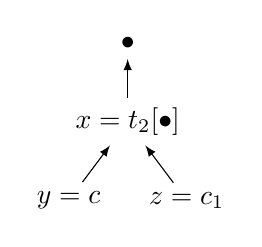
\begin{tikzpicture}[ 
  edge from parent path={(\tikzchildnode\tikzchildanchor) edge [-latex] (\tikzparentnode\tikzparentanchor)},
  level distance=1cm
]
\node (d) {$\bullet$} child{node (a) {$x=t_2[\bullet]$} child{node (b) {$y=c$}} child{node (c)
{$z=c_1$}}};

\end{tikzpicture}
\end{center}
Now each of the environments is represented by a linked list, with the binding
of $x$ shared between them. This is an example of a \emph{shared} environment
~\cite{appel1988optimizing}. This shared, linked structure dates back to the 
first machine for evaluating expressions, Landin's SECD
machine~\cite{landin1964mechanical}.

The drawbacks and advantages of each approach are well known. With a flat
environment, variable lookup can be performed with a simple offset
~\cite{jonesstg,appel1992compiling}. On the other hand, significant
duplication can occur, as I will discuss in Section~\ref{sec:exist}.
With a shared environment, that duplication is removed, but at the cost of
possible link traversal upon dereference. 

As with most topics in compilers and abstract machines, the design space is
actually more complex. For example, Appel and Jim show a wide range of hybrids
~\cite{appel1988optimizing} between the two, and Appel and Shao
~\cite{shao1994space} show an optimized hybrid that aims to achieve the benefits
of both approaches. And as shown in the next section, choice of evaluation
strategy further complicates the picture.

\section{Existing Call-by-Need Environments} \label{sec:exist}

Existing call by need machines use flat environments with a heap of
closures~\cite{jonesstg,TIM,johnsson1984efficient,boquist1997grin}. These
environments may contain some combination of primitive values and pointers into the
heap ($p$ below). The pointers and heap implement the memoization of results
required for call by need. Returning to the earlier example, $(\lambda
x.(\lambda y.t) (\lambda z.t_1)) t_2$, we can view a simplified execution state
for this approach when entering $t$ as follows:

\begin{center}
\textbf{Closure}
\begin{align*}
t[x=p_0, y=p_1] \\
\end{align*}
\textbf{Heap}
\begin{align*}
p_0 &\mapsto t_2[\bullet] \\
p_1 &\mapsto \lambda z.t_1[x=p_0] 
\end{align*}
\end{center}

Consider $t_2[\bullet]$, the closure at $p_0$. If it is not in WHNF (this sort
of unevaluated closure is called a
\emph{thunk}~\cite{ingerman1961way,peyton1992implementing}), then if it is
entered in either the evaluation of $t$ or $t_1$, the resulting value will
overwrite the closure at $p_0$. The result of the computation is then shared
with all other instances of $x$ in $t$ and $t_1$. In the case that terms have a
large number of shared variables, environment duplication can be expensive.
Compile-time transformation ~\cite{peyton1992implementing} (tupling arguments)
helps, but we show that the machine can avoid duplication completely.

Depending on $t$, either or both of the closures created for its free variables
may not be evaluated. Therefore, it is possible that the work of creating the
environment for that thunk will be wasted. This waste is well known, and
existing approaches address it by avoiding thunks as much as possible
~\cite{jonesstg,johnsson1984efficient}. Unfortunately, in cases like the above
example, thunks are necessary. I aim to minimize the cost of creating such
thunks.

Thunks are special in another way.  Recall that one advantage of flat
environments is quick variable lookups. In a lazy language, this advantage is
reduced because \emph{a thunk can only be entered once}. After it is entered, it
is overwritten with a value, so the next time that heap location is entered it
is entered with a value and a different environment. Thus, the work to ensure
that the variable lookup is fast is used for at most one evaluation of the
thunk. This is in contrast to a call-by-value language, in which every closure
is constructed for a value, and can be entered an arbitrary number of times. 

A more subtle drawback of the flat environment representation is that
environments can vary in size, and thus a value in WHNF can be too large to fit
in the space allocated for the thunk it is replacing. This problem is discussed
in~\cite{jonesstg}, where the proposed solution is to put the value closure in
a fresh location in the heap where there is sufficient room. The original
thunk location is then replaced with an indirection to the value at the freshly
allocated location. These indirections are removed during garbage collection,
but do impose some cost, both in runtime efficiency and implementation
complexity~\cite{jonesstg}.

I have thus far ignored a number of details with regard to current
implementations. For example, the STG machine can split the flat environment, so
that part is allocated on the stack and part on the heap.  The TIM allocates its
flat environments separately from its closures so that each closure is a code
pointer, environment pointer pair~\cite{TIM} while the STG machine keeps
environment and code co-located~\cite{jonesstg}. Still, the basic design
principle holds: a flat environment for each closure allows quick variable
indexing, but with an initial overhead.

To summarize, the flat environment representation in a call by need language
implies that whenever a term might be needed, the necessary environment is
constructed from the current environment.  This operation can be expensive, and
it is wasted if the variable is never dereferenced. In this work, I aim to
minimize this potentially unnecessary overhead.

Figure~\ref{fig:designspace} depicts the design space relevant to this chapter.
There are existing call by value machines with both flat and shared
environments, and call by need machines with flat environments. As far as I am
aware, I am the first to use a shared environment to implement lazy evaluation. 

It is worth noting that there has been work on lazy machines that effectively use
linked environments, which could potentially be implemented as a shared
environment, e.g., Sestoft's work on Krivine machines~\cite{sestoft}, but none
make the realization that the shared environment can be used to implement
sharing of results, which is the primary contribution of this chapter.

\begin{figure}
\begin{tabularx}{\textwidth}{l | X | X}
                & Flat Environment     & Shared Environment \\ \hline
  Call by need  & STG~\cite{jonesstg}, 
                  TIM~\cite{TIM}, 
                  GRIN~\cite{boquist1997grin} 
                & $\mathcal{\mathcal{C} \mskip -4mu \mathcal{E}}$ Machine \\
  Call by value & ZAM~\cite{leroy1990zinc}, 
                  SML/NJ~\cite{appel1991standard}
                & ZAM,
                  SECD~\cite{landin1964mechanical}, 
                  SML/NJ \\
\end{tabularx}
\caption{Evaluation strategy and environment structure design space. Each
acronym refers to an existing implementation. Some implementations use multiple
environment representations.}
\label{fig:designspace}
\end{figure}



\chapter{\ce Machine}\label{chap:ce}
\epigraph{The lurking suspicion that something could be simplified is the
world's richest source of rewarding challenges.}{\textit{Edsger Dijkstra}}
In this chapter I define the \ce machine semantics, both big-step and small-step
versions. I try and convey some intuition for why the shared environment
structure works as a technique for sharing results of computation. The
definitions here are the core of both implementations, the native code compiler
in Chapter~\ref{chap:cem} and the verified compiler in
Chapter~\ref{chap:verified}. More specifically, I formalize the connection
between call-by-need evaluation and shared environments in a big-step semantics
(Section~\ref{sec:calc}).  Section~\ref{sec:mach} implements the big-step with a
small-step semantics by adding a context (or stack). I leave the proof that it
is a correct implementation for Chapter~\ref{chap:verified}.

\section{Big-Step \ce} \label{sec:calc}

This section shows how the shared environment approach can be applied to
call-by-need evaluation. It starts with a big step semantics that abstracts away
environment representation, Curien's calculus of closures, and then shows how it
can be modified to force sharing. See Curien's call-by-name calculus of closures
in Figure~\ref{fig:curien}. \footnote{Curien calls it a ``lazy'' evaluator, and
there is some ambiguity with the term lazy, but here the term is used only to
mean call-by-need. Curien's condition checking that $i < m$ is omitted as the
semantics is only defined for closed terms.}

The App rule pushes a closure onto the environment, and the Id rule indexes into
the environment, entering the corresponding closure. This section shows that by
removing ambiguity about how the environments are represented, and forcing them
to be represented in a \emph{cactus stack}~\cite{stenstrom1988vlsi}, we can
define a novel call-by-need big step semantics.

To start, consider again the example from Section~\ref{sec:env}, this time with
de Bruijn indices: $(\lambda(\lambda t) \; (\lambda t_1)) t_2$.  The terms $t$
and $t_1$, when evaluated in Curien's calculus of closures, would have the
following environments, respectively: 

\begin{center}
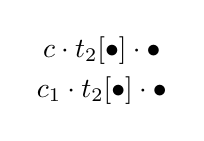
\begin{tikzpicture}
\node {$c \cdot t_2[\bullet] \cdot \bullet$};
\node [yshift=-0.5cm] {$c_1 \cdot t_2[\bullet] \cdot \bullet$};
\end{tikzpicture}
\end{center}

Again, the second closure is identical in each environment.  And again,
we can represent these environments with a shared environment, this time
keeping call-by-need evaluation in mind:
\begin{center}
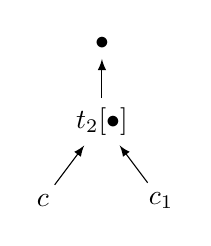
\begin{tikzpicture}[ 
  edge from parent path={(\tikzchildnode\tikzchildanchor) edge [-latex] (\tikzparentnode\tikzparentanchor)},
  level distance=1cm
]
\node (a) {$\bullet$} child{node (d) {$t_2[\bullet]$} child{node (b) {$c$}} child{node (c)
{$c_1$}}};

%\draw let \p1=(a), \p2 =(b), \n1={atan2(\y2-\y1,\x2-\x1)}, \n2={veclen(\y2-\y1,\x2-\x1)}
%  in ($ (a)!0.5!(b) $) ellipse [x radius=\n2/2+10pt, y radius=10pt, rotate=90-\n1];
%\draw let \p1=(a), \p2 =(c), \n1={atan2(\y2-\y1,\x2-\x1)}, \n2={veclen(\y2-\y1,\x2-\x1)}
%  in ($ (a)!0.5!(c) $) ellipse [x radius=\n2/2+10pt, y radius=10pt, rotate=90-\n1];
\end{tikzpicture}
\end{center}
This inverted tree structure seen earlier with the leaves pointing toward the
root is called a \emph{cactus stack} (sometimes called a spaghetti stack or
saguaro stack) when used to implement stacks~\cite{hauck1968burroughs,ichbiah1991rationale}, or a parent pointer tree in
general. In this use case, every node defines an environment as the sequence of
closures in the path to the root.  If $t_2[\bullet]$ is a thunk, and is updated
in place with the value after its first reference, then both environments would
contain the resulting value. This is exactly the kind of sharing that is
required by call-by-need, and thus we can use this structure to build a
call-by-need evaluator. This is the essence of the \ce machine. 

Curien's calculus of closures does not differentiate between flat and shared
environment representations; it has no need to. Therefore, we must derive a new
semantics, forcing the environment to be shared. Because we can hold the closure
directly in the environment, the standard approach of a heap of closures is
replaced with a \emph{heap of environments}. To enforce sharing, we extend
Curien's calculus of closures to explicitly include the heap of environments,
which we refer to as a \emph{cactus environment}. This is effectively a parent
pointer tree in which the contained objects are closures. 

See Figure~\ref{fig:bigstep} for the syntax and semantics of the \ce big step
semantics. Recall that we are only concerned with evaluation of closed terms.
The initial closed term $t$ is placed in a $(t[0],\epsilon[0 \mapsto \bullet])$
configuration, and evaluation terminates on a value. Some shorthand is used to
make heap notation more palatable for both the big-step semantics presented here
and the small step semantics presented in the next section. $\mu(l,i)=l' \mapsto
c \cdot l''$ denotes that looking up the $i$'th element in the linked
environment structure starting at $l$ results in location $l'$, where closure
$c$ and continuing environment $l''$ reside. $\mu(l) = c \cdot l'$ is the
statement that $l \mapsto c \cdot l' \in \mu$, and $\mu(u \mapsto c \cdot l')$
is $\mu$ with location $u$ updated to map to $c \cdot e$. Two 
different semantics are defined, one for call-by-name
(Figure~\ref{fig:bigstepname}) and one for call-by-need
(Figure~\ref{fig:bigstep}), which makes the connection to Curien's call-by-name
calculus more straightfoward. The rule for application is identical for both
semantics: each evaluates the left hand side to a function, then binds the
variable in the cactus environment, extending the current environment.

\begin{figure}
\textbf{Syntax}
\begin{align*}
\tag{Term} t &::= i \; | \; \lambda t \; | \; t \; t  \\
\tag{Variable} i &\in \mathbb{N}  \\
\tag{Closure} c &::= t \left[l\right] \\
\tag{Value} v &::= \lambda t \left[l\right] \\
\tag{Heap} \mu &::= \epsilon \; | \; \mu \left[ l \mapsto \rho \right] \\
\tag{Environment} \rho &::= \bullet \; | \; c \cdot l \\
\tag{Location} l,f &\in \mathbb{N}  \\
\tag{Configuration} s &::= \left(c, \mu \right)
\end{align*}
\textbf{Semantics}
\begin{align*}
\tag{Id} \inference
{\mu \left( l, i \right) = l' \mapsto c \cdot l'' \quad 
 \left(c, \mu\right) \Downarrow \left(v, \mu'\right)}
{\left(i\left[l\right],\mu\right) \Downarrow \left(v, \mu'\right)}
\end{align*} 
\begin{align*}
\tag{App} \inference
{\left(t\left[l\right], \mu\right) \Downarrow \left(\lambda t_2\left[l'\right], \mu'\right) 
   \quad f \not \in \textnormal{dom}\left(\mu'\right)
   \\ \left(t_2\left[f\right], \mu'\left[f \mapsto t_3\left[l\right] \cdot l'\right]\right)
         \Downarrow 
      \left(v, \mu'' \right) 
   }
{\left(t \; t_3\left[l\right], \mu\right) \Downarrow \left(v, \mu'' \right)}  
\end{align*} 
\begin{align*}
\tag{Abs} \inference {} {\left(\lambda t\left[l\right], \mu\right) \Downarrow \left(\lambda t\left[l\right], \mu\right)}
\end{align*}
\caption{Big-step call-by-name \ce syntax and semantics}
\label{fig:bigstepname}
\end{figure}


The only difference between this semantics and Curien's is that if we need
to extend an environment multiple times, the semantics \emph{requires}
sharing it among the extensions. This makes no difference for call-by-name, but
it is needed for the sharing of results in the Id rule. The explicit
environment sharing ensures that the closure that is overwritten with a
value is shared correctly.

\begin{figure}
\textbf{Syntax}
\begin{align*}
\tag{Term} t &::= i \; | \; \lambda t \; | \; t \; t  \\
\tag{Variable} i &\in \mathbb{N}  \\
\tag{Closure} c &::= t \left[l\right] \\
\tag{Value} v &::= \lambda t \left[l\right] \\
\tag{Heap} \mu &::= \epsilon \; | \; \mu \left[ l \mapsto \rho \right] \\
\tag{Environment} \rho &::= \bullet \; | \; c \cdot l \\
\tag{Location} l,f &\in \mathbb{N}  \\
\tag{Configuration} s &::= \left(c, \mu \right)
\end{align*}
\textbf{Semantics}
\begin{align*}
\tag{Id} \inference
{\mu \left( l, i \right) = l' \mapsto c \cdot l'' \quad 
 \left(c, \mu\right) \Downarrow \left(v, \mu'\right)}
{\left(i\left[l\right],\mu\right) \Downarrow \left(v, \mu'\left[l' \mapsto v \cdot l''\right]\right)}
\end{align*}
\begin{align*}
\tag{App} \inference
{\left(t\left[l\right], \mu\right) \Downarrow \left(\lambda t_2\left[l'\right], \mu'\right) 
   \quad f \not \in \textnormal{dom}\left(\mu'\right)
   \\ \left(t_2\left[f\right], \mu'\left[f \mapsto t_3\left[l\right] \cdot l'\right]\right)
         \Downarrow 
      \left(v, \mu'' \right) 
   }
{\left(t \; t_3\left[l\right], \mu\right) \Downarrow \left(v, \mu'' \right)}  
\end{align*}
\begin{align*}
\tag{Abs} \inference {} {\left(\lambda t\left[l\right], \mu\right) \Downarrow \left(\lambda t\left[l\right], \mu\right)}
\end{align*}
\caption{Big-step call-by-need \ce syntax and semantics}
\label{fig:bigstep}
\end{figure}


\section{Small-Step \ce} \label{sec:mach}

Using the calculus of cactus environments defined in the previous section, we
derive an abstract machine: the \ce machine. The syntax and semantics are
defined in Figure~\ref{fig:cesm}. 

\begin{figure}
\textbf{Syntax}
\begin{align*}
\tag{State} s &::= \langle c, \sigma, \mu \rangle \\
\tag{Term} t &::= i \; | \; \lambda t \; | \; t \; t  \\
\tag{Variable} i &\in \mathbb{N}  \\
\tag{Closure} c &::= t \left[l\right] \\
\tag{Value} v &::= \lambda t\left[l\right] \\
\tag{Heap} \mu &::= \epsilon \; | \; \mu \left[ l \mapsto \rho \right] \\
\tag{Environment} \rho &::= \bullet \; | \; c \cdot l \\
\tag{Stack} \sigma &::= \square \; | \; \sigma \; c \;  | \; \sigma \; u \\
\tag{Location} l,u,f &\in \mathbb{N}
\end{align*}
\textbf{Semantics}
\begin{align*}
\tag{Upd}
\langle v,  \sigma \; u , \mu \rangle 
  &\rightarrow
\langle v, \sigma, \mu\left(u \mapsto v \cdot l\right) \rangle  
\; \textnormal{where} \; c \cdot l = \mu\left(u\right) \\
\tag{Lam}
\langle \lambda t\left[l\right], \sigma \; c, \mu \rangle 
  &\rightarrow
\langle t\left[f\right], \sigma, \mu\left[f \mapsto c \cdot l\right]\rangle f
\not \in \textnormal{dom}\left(\mu\right)  \\
\tag{App}
\langle t \; t'\left[l\right], \sigma, \mu \rangle
  &\rightarrow
\langle t\left[l\right], \sigma \; t'\left[l\right], \mu \rangle \\
\tag{Var}
\langle i\left[l\right], \sigma, \mu \rangle
  &\rightarrow
\langle c, \sigma \; l'', \mu \rangle
\; \textnormal{where} \; l'' \mapsto c \cdot l' = \mu\left(l, i\right)
\end{align*}
\caption{Small-step \ce syntax and semantics}
\label{fig:cesm}
\end{figure}

The small-step semantics operate identically to the big-step, extended only with
a context to implement the updates from the Id subderivation ($\sigma \; u$) and
the operands from the App subderivation ($\sigma \; c$).  Much like the
calculus, a term $t$ is inserted into an initial state $\langle t[0], \sigma,
\epsilon[0\mapsto\bullet]\rangle$ . On the update rule, the current closure is a
value, and there is an update marker as the outermost context.  This implies
that a variable was entered and that the current closure represents the
corresponding value for that variable. Thus, we update the location $u$ that the
variable entered, replacing whatever term was entered with the current closure.
The Lam rule takes an argument off the context and binds it to a variable,
allocating a fresh heap location for the bound variable. This ensures that every
instance of the variable will point to this location, and thus the bound term
will be evaluated at most once. The App rule simply pushes an argument term in
the current environment. The Var rule enters the closure pointed to by the
\textit{i}'th environment location.  

To get some intuition for the $\mathcal{\mathcal{C} \mskip -4mu \mathcal{E}}$
machine and how it works, consider Figure~\ref{fig:state}, evaluation of the
term $(\lambda a.(\lambda b.b \; a) \lambda c.c \; a) \; ((\lambda i.i)
\lambda j.j)$, or $(\lambda(\lambda0\;1)\;\lambda0\;1)\;((\lambda0)\;
\lambda0)$ with deBruijn indices.

\begin{figure}
\scriptsize
\begin{align*}
&\langle (\lambda(\lambda0\;1)\;\lambda0\;1)\;((\lambda0)\;\lambda0)[0],\square,\epsilon[0\mapsto\bullet]\rangle\\
&\rightarrow_{\mathcal{\mathcal{C} \mskip -4mu \mathcal{E}}}\langle \lambda(\lambda0\;1)\;\lambda0\;1[0],\square (\lambda0)\;\lambda0[0],\epsilon[0\mapsto\bullet]\rangle\\ 
&\rightarrow_{\mathcal{\mathcal{C} \mskip -4mu \mathcal{E}}}\langle (\lambda0\;1)\;\lambda0\;1[1],\square,\epsilon[0\mapsto\bullet][1\mapsto(\lambda0)\;\lambda0[0]\cdot0]\rangle\\ 
&\rightarrow_{\mathcal{\mathcal{C} \mskip -4mu \mathcal{E}}}\langle \lambda0\;1[1],\square \lambda0\;1[1],\epsilon[0\mapsto\bullet][1\mapsto(\lambda0)\;\lambda0[0]\cdot0]\rangle\\ 
&\rightarrow_{\mathcal{\mathcal{C} \mskip -4mu \mathcal{E}}}\langle 0\;1[2],\square,\epsilon[0\mapsto\bullet][1\mapsto(\lambda0)\;\lambda0[0]\cdot0][2\mapsto\lambda0\;1[1]\cdot1]\rangle\\ 
&\rightarrow_{\mathcal{\mathcal{C} \mskip -4mu \mathcal{E}}}\langle 0[2],\square 1[2],\epsilon[0\mapsto\bullet][1\mapsto(\lambda0)\;\lambda0[0]\cdot0][2\mapsto\lambda0\;1[1]\cdot1]\rangle\\ 
&\rightarrow_{\mathcal{\mathcal{C} \mskip -4mu \mathcal{E}}}\langle \lambda0\;1[1],\square 1[2] 2,\epsilon[0\mapsto\bullet][1\mapsto(\lambda0)\;\lambda0[0]\cdot0][2\mapsto\lambda0\;1[1]\cdot1]\rangle\\ 
&\rightarrow_{\mathcal{\mathcal{C} \mskip -4mu \mathcal{E}}}\langle \lambda0\;1[1],\square 1[2],\epsilon[0\mapsto\bullet][1\mapsto(\lambda0)\;\lambda0[0]\cdot0][2\mapsto\lambda0\;1[1]\cdot1]\rangle\\ 
&\rightarrow_{\mathcal{\mathcal{C} \mskip -4mu \mathcal{E}}}\langle 0\;1[3],\square,\epsilon[0\mapsto\bullet][1\mapsto(\lambda0)\;\lambda0[0]\cdot0][2\mapsto\lambda0\;1[1]\cdot1][3\mapsto1[2]\cdot1]\rangle\\ 
&\rightarrow_{\mathcal{\mathcal{C} \mskip -4mu \mathcal{E}}}\langle 0[3],\square 1[3],\epsilon[0\mapsto\bullet][1\mapsto(\lambda0)\;\lambda0[0]\cdot0][2\mapsto\lambda0\;1[1]\cdot1][3\mapsto1[2]\cdot1]\rangle\\ 
&\rightarrow_{\mathcal{\mathcal{C} \mskip -4mu \mathcal{E}}}\langle 1[2],\square 1[3] 3,\epsilon[0\mapsto\bullet][1\mapsto(\lambda0)\;\lambda0[0]\cdot0][2\mapsto\lambda0\;1[1]\cdot1][3\mapsto1[2]\cdot1]\rangle\\ 
&\rightarrow_{\mathcal{\mathcal{C} \mskip -4mu \mathcal{E}}}\langle 0[1],\square 1[3] 3,\epsilon[0\mapsto\bullet][1\mapsto(\lambda0)\;\lambda0[0]\cdot0][2\mapsto\lambda0\;1[1]\cdot1][3\mapsto1[2]\cdot1]\rangle\\ 
&\rightarrow_{\mathcal{\mathcal{C} \mskip -4mu \mathcal{E}}}\langle (\lambda0)\;\lambda0[0],\square 1[3] 3 1,\epsilon[0\mapsto\bullet][1\mapsto(\lambda0)\;\lambda0[0]\cdot0][2\mapsto\lambda0\;1[1]\cdot1][3\mapsto1[2]\cdot1]\rangle\\ 
&\rightarrow_{\mathcal{\mathcal{C} \mskip -4mu \mathcal{E}}}\langle \lambda0[0],\square 1[3] 3 1 \lambda0[0],\epsilon[0\mapsto\bullet][1\mapsto(\lambda0)\;\lambda0[0]\cdot0][2\mapsto\lambda0\;1[1]\cdot1][3\mapsto1[2]\cdot1]\rangle\\ 
&\rightarrow_{\mathcal{\mathcal{C} \mskip -4mu \mathcal{E}}}\langle 0[4],\square 1[3] 3 1,\epsilon[0\mapsto\bullet][1\mapsto(\lambda0)\;\lambda0[0]\cdot0][2\mapsto\lambda0\;1[1]\cdot1][3\mapsto1[2]\cdot1][4\mapsto\lambda0[0]\cdot0]\rangle\\ 
&\rightarrow_{\mathcal{\mathcal{C} \mskip -4mu \mathcal{E}}}\langle \lambda0[0],\square 1[3] 3 1 4,\epsilon[0\mapsto\bullet][1\mapsto(\lambda0)\;\lambda0[0]\cdot0][2\mapsto\lambda0\;1[1]\cdot1][3\mapsto1[2]\cdot1][4\mapsto\lambda0[0]\cdot0]\rangle\\ 
&\rightarrow_{\mathcal{\mathcal{C} \mskip -4mu \mathcal{E}}}\langle \lambda0[0],\square 1[3] 3 1,\epsilon[0\mapsto\bullet][1\mapsto(\lambda0)\;\lambda0[0]\cdot0][2\mapsto\lambda0\;1[1]\cdot1][3\mapsto1[2]\cdot1][4\mapsto\lambda0[0]\cdot0]\rangle\\ 
&\rightarrow_{\mathcal{\mathcal{C} \mskip -4mu \mathcal{E}}}\langle \lambda0[0],\square 1[3] 3,\epsilon[0\mapsto\bullet][1\mapsto\lambda0[0]\cdot0][2\mapsto\lambda0\;1[1]\cdot1][3\mapsto1[2]\cdot1][4\mapsto\lambda0[0]\cdot0]\rangle\\ 
&\rightarrow_{\mathcal{\mathcal{C} \mskip -4mu \mathcal{E}}}\langle \lambda0[0],\square 1[3],\epsilon[0\mapsto\bullet][1\mapsto\lambda0[0]\cdot0][2\mapsto\lambda0\;1[1]\cdot1][3\mapsto\lambda0[0]\cdot1][4\mapsto\lambda0[0]\cdot0]\rangle\\ 
&\rightarrow_{\mathcal{\mathcal{C} \mskip -4mu \mathcal{E}}}\langle 0[5],\square,\epsilon[0\mapsto\bullet][1\mapsto\lambda0[0]\cdot0][2\mapsto\lambda0\;1[1]\cdot1][3\mapsto\lambda0[0]\cdot1][4\mapsto\lambda0[0]\cdot0][5\mapsto1[3]\cdot0]\rangle\\ 
&\rightarrow_{\mathcal{\mathcal{C} \mskip -4mu \mathcal{E}}}\langle 1[3],\square 5,\epsilon[0\mapsto\bullet][1\mapsto\lambda0[0]\cdot0][2\mapsto\lambda0\;1[1]\cdot1][3\mapsto\lambda0[0]\cdot1][4\mapsto\lambda0[0]\cdot0][5\mapsto1[3]\cdot0]\rangle\\ 
&\rightarrow_{\mathcal{\mathcal{C} \mskip -4mu \mathcal{E}}}\langle 0[1],\square 5,\epsilon[0\mapsto\bullet][1\mapsto\lambda0[0]\cdot0][2\mapsto\lambda0\;1[1]\cdot1][3\mapsto\lambda0[0]\cdot1][4\mapsto\lambda0[0]\cdot0][5\mapsto1[3]\cdot0]\rangle\\ 
&\rightarrow_{\mathcal{\mathcal{C} \mskip -4mu \mathcal{E}}}\langle \lambda0[0],\square 5 1,\epsilon[0\mapsto\bullet][1\mapsto\lambda0[0]\cdot0][2\mapsto\lambda0\;1[1]\cdot1][3\mapsto\lambda0[0]\cdot1][4\mapsto\lambda0[0]\cdot0][5\mapsto1[3]\cdot0]\rangle\\ 
&\rightarrow_{\mathcal{\mathcal{C} \mskip -4mu \mathcal{E}}}\langle \lambda0[0],\square 5,\epsilon[0\mapsto\bullet][1\mapsto\lambda0[0]\cdot0][2\mapsto\lambda0\;1[1]\cdot1][3\mapsto\lambda0[0]\cdot1][4\mapsto\lambda0[0]\cdot0][5\mapsto1[3]\cdot0]\rangle\\ 
&\rightarrow_{\mathcal{\mathcal{C} \mskip -4mu \mathcal{E}}}\langle \lambda0[0],\square,\epsilon[0\mapsto\bullet][1\mapsto\lambda0[0]\cdot0][2\mapsto\lambda0\;1[1]\cdot1][3\mapsto\lambda0[0]\cdot1][4\mapsto\lambda0[0]\cdot0][5\mapsto\lambda0[0]\cdot0]\rangle
\end{align*}
\caption{$\mathcal{\mathcal{C} \mskip -4mu \mathcal{E}}$ machine example.
Evaluation of $(\lambda(\lambda0\;1)\;\lambda0\;1)\;((\lambda0)\;\lambda0)$}
\label{fig:state}
\end{figure}



\chapter{Native Code Compilation}\label{chap:cem}
\epigraph{Much of my work has come from being lazy.}{\textit{John Backus}}
Existing implementations of call-by-need take care in \emph{packaging} a delayed
computation, or \emph{thunk}, by building a closure with an array that contains
the bindings of all free variables \cite{jonesstg,boquist1997grin}. The overhead
induced by this operation is well known, and is one reason existing
implementations avoid thunks wherever possible \cite{johnsson1984efficient}. The
key insight of our Cactus Environment (\ce) Machine is that this overhead can be
minimized by only recording a location in a shared environment.

As an example, consider the application $f \; e$. In existing call-by-need
implementations, e.g., the STG machine\cite{jonesstg}, a closure with a flat
environment will be constructed for $e$.  Doing so incurs a time and memory cost
proportional to the number of free variables of $e$. \footnote{In some
implementations, these are lambda-lifted to be formal parameters, but the
principle is the same.} We minimize this packaging cost by recording a
location in a shared environment, which requires only two
machine words (and two instructions) for the thunk: one for the code pointer,
and one for the environment pointer. One way to think about the approach is that
it is \emph{lazier} about lazy evaluation: in the case that $e$ is unneeded, the
work to package it in a thunk is entirely wasted. In the spirit of lazy
evaluation, we attempt to minimize this potentially unnecessary work.  

This chapter presents a simple implementation of the \ce machine that
compiles a simple lazy functional language to x86\_64 assembly. In addition, it
presents a preliminary evaluation that shows performance comparable to existing
implementations (Sections~\ref{sec:impl} and~\ref{sec:eval}). 

Section~\ref{sec:impl} describes a straightforward implementation of \ce,
extended with machine literals and primitive operations, and compiling directly
to native code. Section~\ref{sec:eval} evaluates the implementation, showing
that it is capable of performing comparably to existing implementations despite
lacking several common optimizations, and discusses the results.
Section~\ref{sec:disc} discusses related work, limitations of the approach, and
some ideas for future work.

\section{Implementation} \label{sec:impl}

This section describes how the $\mathcal{\mathcal{C} \mskip -4mu \mathcal{E}}$
machine can be mapped directly to x86\_64 insructions. Specifically, we re-define
the three instructions given by the TIM~\cite{TIM}: \texttt{TAKE},
\texttt{ENTER}, and \texttt{PUSH}, and implement them with x86\_64 assembly. We
also describe several design decisions, as well as some optimizations. All
implementation and benchmark code is available at
\texttt{http://cs.unm.edu/\textasciitilde stelleg/cem-tfp2016.tar.gz}.

Each closure is represented as a $\langle$code pointer, environment
pointer$\rangle$ tuple. The
Context is implemented as a stack, with updates represented as a $\langle$null pointer,
environment pointer$\rangle$ tuple to differentiate them from closure arguments. The
Heap, or cactus environment, is implemented as a heap containing $\langle$closure,
environment pointer$\rangle$ structs. As a result, each cell in the heap takes 3
machine words.

\subsection{Compilation}
The three instructions are given below, with descriptions of their behavior. 

\begin{itemize}
\item \texttt{TAKE}: Pops a context item off the stack. If the item is an
update $u$, the instruction updates the location $u$ with the current closure.
If it is an argument $c$, the instruction binds the closure $c$ to the fresh
location in the cactus environment.
\item \texttt{ENTER i}: Enters the closure defined by variable index \texttt{i},
the current environment pointer, and the current cactus environment.  \item
\texttt{PUSH m}: Pushes the code location \texttt{m} along with the
current environment pointer. 
\end{itemize}

Each of these instructions corresponds directly to a corresponding lambda term:
abstraction compiles to \texttt{TAKE}, application to \texttt{PUSH}, and
variables to \texttt{ENTER}. Each is compiled using a direct implementation of
the transition functions of the $\mathcal{\mathcal{C} \mskip -4mu \mathcal{E}}$
machine. The mapping from lambda terms can be seen in
Figure~\ref{fig:cemcompile}, which defines the compiler. Unlike the TIM, our
version of \texttt{TAKE} doesn't have an arity; we compile a sequence of
lambdas as a sequence of \texttt{TAKE} instructions.  While we have not
compared performance of the two approaches directly, we suspect that \texttt{n}
inlined \texttt{TAKE} instructions should be roughly as fast as a \texttt{TAKE
n} instruction.  Similarly, the \texttt{ENTER i} instruction can be implemented
either as a loop or unrolled, depending on \texttt{i}, and more performance
comparisons are needed to determine the trade-off between code size and speed.

\begin{figure}
\begin{align*} C[\![t \; t']\!] &= \texttt{PUSH}\;label_{C[\![t']\!]}:C[\![t]\!] \concat C[\![t']\!] \\
C[\![\lambda t]\!] &= \texttt{TAKE}:C[\![t]\!] \\
C[\![i]\!] &= \texttt{ENTER} \; i
\end{align*}
\caption{$\mathcal{\mathcal{C} \mskip -4mu \mathcal{E}}$ machine compilation scheme. $C$ compiles a sequence of
instructions from a term. The $label$ represents a code label: each instruction
is given a unique label. The $:$ operator denotes prepending an item to a
sequence and $\concat$ denotes concatenating two sequences.}
\label{fig:cemcompile}
\end{figure}

We compile to x86\_64 assembly. Each of the three instructions is mapped onto
x86\_64 instructions with a macro. The \texttt{PUSH} instruction is particularly
simple, consisting of only two x86\_64 instructions (two \texttt{push}es, one for
the code pointer and one for the environment pointer). This is actually an
important point: \emph{thunk creation is only two hardware instructions,
regardless of environment size}.  

\subsection{Machine Literals and Primitive Operations}

Following Sestoft~\cite{sestoft}, we extend the $\mathcal{\mathcal{C} \mskip -4mu \mathcal{E}}$ machine to
include machine literals and primitive operations. Figure~\ref{fig:extsyntax}
shows the parts of syntax and semantics that are new or modified. 

\begin{figure}
\textbf{Syntax}
\begin{align*}
\tag{Term}    t &::= i \; | \; \lambda t \; | \; t \; t | \; n \; | \; op \\
\tag{Integer} n &\in \mathbb{I} \\
\tag{PrimOp} op &::= + \; | \; - \; | \; * \; | \; \; / \;\; | \; = \; | \; > \; | \; < \\
\tag{Value} v &::= \lambda t[l] \; | \; n[l] \\
\end{align*}
\textbf{Integer and Primop Semantics}
\begin{align*}
\tag{Int}
\langle n[l], \sigma \; c, \mu, k \rangle
  &\rightarrow
\langle c, \sigma \; n[l], \mu, k \rangle \\
\tag{Op} 
\langle op[l], \sigma \; n' \; n, \mu, k \rangle
  &\rightarrow
\langle op(n',n)[l], \sigma, \mu, k \rangle
\end{align*}
\caption{Extensions to the syntax and semantics of the small-step \ce semantics.}
\label{fig:extsyntax}
\end{figure}

\subsection{Omitted Extensions}

Our implementation omits a few other standard extensions. Here we address some
of these omissions.

Data types are a common extension that we omit ~\cite{jonesstg,boquist1997grin}.
We take the approach of Sestoft ~\cite{sestoft} that these can be efficiently
implemented with pure lambda terms. For example, consider a list data type (in
Haskell syntax): \texttt{data List a = Cons a (List a) | Nil}. This can be
represented in pure lambda terms with $\mathit{Cons} = \lambda h.\lambda t.\lambda
c.\lambda n.c \; h \; t$ and $\mathit{Nil} = \lambda c.\lambda n.n$. 

Let bindings are another term commonly included in functional language
compilers, even in the internal representation ~\cite{boquist1997grin,jonesstg}.
Non-recursive let is syntactic sugar for a lambda binding and application, and
we treat it as such. This approach helps ensure that we can of
compile arbitrary lambda terms, while some approaches require pre-processing
~\cite{sestoft,TIM}.

Recursive let bindings are a third omission. Here we follow Rozas
~\cite{rozas1992taming}: If it can be represented in pure lambda terms, it should
be. Thus, we implement recursion using the standard Y combinator. In the case of
mutual recursion, we use the Y combinator in conjunction with a church tuple of
the mutually recursive functions. Without the appropriate optimizations
~\cite{rozas1992taming}, this approach has high overhead, as we discuss in
Section~\ref{sec:res}.

\subsection{Optimizations}

The $\mathcal{C} \mskip -4mu \mathcal{E}$ implementation described in the previous section is 
completely unoptimized. For example, no effort is expended to
discover global functions to avoid costly jumps to pointers in the heap
~\cite{jonesstg}. Indeed, every variable reference will look up the code pointer
in the shared environment and jump to it. There is also no implementation of 
control flow analysis as used by Rozas to optimize away the Y combinator.  Thus,
every recursive call exhibits the large overhead involved in re-calculating the
fixed point of the function.  

We do, however, implement two basic optimizations, primarily to reduce the load
on the heap:

\begin{itemize}
\item \texttt{POP}: A \texttt{TAKE} instruction can be converted to a \texttt{POP}
instruction that throws away the operand on the top of the stack if there are no
variables bound to the $\lambda$ term in question. For example, the function
$\lambda x.\lambda y.x$ can be implemented with \texttt{TAKE}, \texttt{POP},
\texttt{ENTER 0}.  
\item \texttt{ENTERVAL}: An \texttt{ENTER} instruction, when entering a
closure that is already a value, should not push an update marker onto the
stack. This shortcut prevents unnecessary writes to the stack and heap
~\cite{jonesstg,lkm,sestoft}.  
\end{itemize}

\subsection{Garbage Collection}

We have implemented a simple mark and sweep garbage collector with the property
that it does not require two spaces because constant-sized closures in the
heap allow a linked-list representation for the free cells. Indeed,
while the abstract machine from Section~\ref{sec:mach} increments a free heap
counter, the actual implementation uses the next free cell in the linked list.

Because the focus of this chapter is not on the performance of garbage collection,
we ensure the benchmarks in Section~\ref{sec:eval} are not dominated by GC time.


\section{Performance Evaluation} \label{sec:eval}

This section reports experiments that assess the strengths and weaknesses of
the $\mathcal{\mathcal{C} \mskip -4mu \mathcal{E}}$ machine. We evaluate using benchmarks from the \texttt{nofib}
benchmark suite. Because we have implemented only machine integers, and must
translate the examples by hand, we use a subset of the \texttt{nofib} suite that
excludes floating point values and arrays. A list of the benchmarks used and a
brief description is given in Figure~\ref{fig:bench}.

\begin{figure}
\begin{itemize}
\item \textbf{exp3:} A Peano arithmetic benchmark. Computes $3^8$ and prints the result. 
\item \textbf{queens:} Computes the number of solutions to the nqueens problem
for an n by n board.
\item \textbf{primes:} A simple primes sieve that computes the nth prime.
\item \textbf{digits-of-e1:} A calculation of the first $n$ digits of $e$ using
continued fractions. 
\item \textbf{digits-of-e2:} Another calculation of the first $n$ digits of $e$ using an
infinite series.  
\item \textbf{fib:} Naively computes the nth Fibonacci number.
\item \textbf{fannkuch:} Counts the number of reverses of a subset of a list.
\item \textbf{tak:} A synthetic benchmark involving basic recursion.
\end{itemize}
\caption{Description of Benchmarks}
\label{fig:bench}
\end{figure}

We compare the $\mathcal{\mathcal{C} \mskip -4mu \mathcal{E}}$ machine with two existing implementations:

\begin{itemize}
\item GHC: The Glasgow Haskell compiler. A high performance, optimizing compiler
based on the STG machine \cite{jonesstg}.
\item UHC: The Utrecht Haskell compiler. An optimizing compiler based on the
GRIN machine \cite{boquist1997grin,dijkstra2009architecture}.
\end{itemize}

We use GHC version 7.10.3 and UHC version 1.1.9.3. We compile with -O0 and -O3,
and show the results for both. Where possible, we pre-allocate a heap of 1GB 
to avoid measuring the performance of GC implementations. The tests were run on
an Intel(R) Xeon(R) CPU E5-4650L at 2.60GHz, running Linux version 3.16. 

\subsection{Results} \label{sec:res}

Figure~\ref{fig:res} gives the benchmark results.  In general, the compiler is
outperformed by GHC, sometimes significantly, and outperforms UHC. I spend the
remainder of the section analyzing these performance differences.

\begin{figure*}
\centering
\begin{tabularx}{\textwidth}{l | X | X | X | X | X}
& $\mathcal{\mathcal{C} \mskip -4mu \mathcal{E}}$ & GHC -O0 & UHC -O0 & GHC -O3 & UHC -O3 \\
\hline
\texttt{exp3 8} & 1.530 & 1.176 & 3.318 & 1.038 & 2.286 \\
\texttt{tak 16 8 0} & 0.366 & 0.146 & 1.510 & 0.006 & 1.416 \\
\texttt{primes 1500} & 0.256 & 0.272 & 1.518 & 0.230 & 1.532 \\
\texttt{queens 9} & 0.206 & 0.050 & 0.600 & 0.012 & 0.598 \\
\texttt{fib 35} & 2.234 & 0.872 & 10.000 & 0.110 & 8.342 \\
\texttt{digits-of-e1 1000} & 3.576 & 1.274 & 21.938 & 0.118 & 22.010 \\
\texttt{digits-of-e2 1000} & 0.404 & 0.792 & 3.430 & 0.372 & 3.278 \\
\texttt{fannkuch 8} & 0.560 & 0.084 & 2.184 & 0.048 & 2.196 \\
\end{tabularx}
\caption{Machine Literals Benchmark Results. Measurement is wall clock time,
units are seconds. Times averaged over 5 runs ($\sigma < 20\%$).}
\label{fig:res}
\end{figure*}

There are many optimizations built into the abstract machine underlying GHC,
but profiling indicates that three in particular lead to much of the performance
disparity: 

\begin{itemize}
\item \textbf{Register allocation:} The $\mathcal{\mathcal{C} \mskip -4mu \mathcal{E}}$ machine has no register
allocator. In contrast, by passing arguments to functions in registers, GHC
avoids much heap thrashing.
\item \textbf{Unpacked literals:} This allows GHC to keep machine literals
without tags in registers for tight loops. In contrast, the $\mathcal{\mathcal{C} \mskip -4mu \mathcal{E}}$
machine operates entirely on the stack, and has a code pointer associated with
every machine literal. 
\item \textbf{Y combinator:} Because recursion in the $\mathcal{\mathcal{C} \mskip -4mu \mathcal{E}}$ machine is
implemented with a Y combinator, it performs poorly. This could be alleviated
with control flow analysis techniques, similar to those used by Rozas~\cite{rozas1992taming}. 
\end{itemize}

Lack of register allocation is the primary current limitation of the $\mathcal{\mathcal{C} \mskip -4mu \mathcal{E}}$
machine. The STG machine pulls the free variables into registers, allowing tight
loops with effective register allocation. However, it is less clear how to
effectively allocate registers in a fully shared environment setting.  That
said, its possible that being lazier about register allocation, e.g., not
loading values into registers that may not be used, could have some performance
benefits.

To isolate the effect of register allocation and unpacked machine
literals, machine integers are replaced with Church numerals in a compatible
subset of the evaluation programs. Figure~\ref{fig:res-church} shows the
performance results with this modification, with the $\mathcal{\mathcal{C}
\mskip -4mu \mathcal{E}}$ machine occasionally even outperforming optimized GHC.

\begin{figure*}
\centering
\begin{tabularx}{\textwidth}{l | X | X | X | X | X}
& $\mathcal{\mathcal{C} \mskip -4mu \mathcal{E}}$ & GHC -O0 & UHC -O0 & GHC -O3 & UHC -O3 \\
\hline
\texttt{tak 14 7 0} & 1.610 & 2.428 & 7.936 & 1.016 & 7.782 \\
\texttt{primes 32} & 0.846 & 1.494 & 4.778 & 0.666 & 5.290 \\
\texttt{queens 8} & 0.242 & 0.374 & 1.510 & 0.154 & 1.508 \\
\texttt{fib 23} & 0.626 & 0.940 & 5.026 & 0.468 & 5.336 \\
\texttt{digits-of-e2 6} & 0.138 & 1.478 & 5.056 & 0.670 & 5.534 \\
\texttt{fannkuch 7} & 0.142 & 0.124 & 0.796 & 0.040 & 0.808 \\
\end{tabularx}
\caption{Church Numeral Benchmark Results. Measurement is wall clock time, 
units are seconds. Times averaged over 5 runs ($\sigma < 20\%$).}
\label{fig:res-church}
\end{figure*}

Next, I consider the disparity due to the Y-combinator, by running a simple
exponentiation example with Church numerals, calculating $3^8 - 3^8 = 0$. In
this case, the $\mathcal{\mathcal{C} \mskip -4mu \mathcal{E}}$ machine
significantly outperforms both GHC and UHC, as seen in
Figure~\ref{fig:res-church-exp} .

\begin{figure*}
\begin{tabularx}{\textwidth}{l | X | X | X | X | X}
& $\mathcal{\mathcal{C} \mskip -4mu \mathcal{E}}$ & GHC -O0 & UHC -O0 & GHC -O3 & UHC -O3 \\
\hline
\texttt{pow 3 8} & 0.564 & 1.994 & 4.912 & 0.906 & 4.932 \\
\end{tabularx}
\caption{Church Numeral Exponentiation Benchmark Results. Measurement is wall clock time, 
units are seconds. Times averaged over 5 runs ($\sigma < 20\%$).}
\label{fig:res-church-exp}
\end{figure*}

These results give us confidence that by adding the optimizations mentioned
above, among others, the $\mathcal{\mathcal{C} \mskip -4mu \mathcal{E}}$ machine has the potential to be the
basis of a real-world compiler. Section~\ref{sec:disc} discusses how some of
these optimizations can be applied to the \ce machine.

\subsection{The Cost of the Cactus}

Recall that variable lookup is linear in the index of the variable, following
pointers until the index is zero. As one might guess, the lookup cost is high.
For example, for the queens benchmark without any optimizations, variable lookup
took roughly $80-90\%$ of the $\mathcal{\mathcal{C} \mskip -4mu \mathcal{E}}$ machine runtime, as measured
by profiling. Much of that cost was for lookups of known combinators, however,
so for the benchmarks above the inlining mentioned in the previous section was
incorporated. Still, even with this simple optimization, variable lookup takes
roughly $50\%$ of execution time. There is some variation across benchmarks, but
this is a rough approximation for the average cost. Section~\ref{sec:disc}
discusses how this cost could be addressed in future work.



\section{Discussion and Related Work} \label{sec:disc}

This section compares the compiler presented in this chapter with existing work,
and discusses areas for future work.

\subsection{Closure Representation}
Appel and Shao \cite{shao1994space} and Appel and Jim \cite{appel1988optimizing}
both cover the design space for closure representation, and develop an approach
called \emph{safely linked closures}. The approach uses flat closures when
there is no duplication, and links in a way that preserves liveness, to prevent
violation of the \emph{safe for space complexity} (SSC) rule
\cite{shao1994space}. While we do not address SSC or garbage collection in
general, understanding the relationship between SSC and shared environment
call-by-need is an interesting area for future work. In particular, hot
environments with no sharing could benefit greatly from replacing shared
structure with flat.

\subsection{Eval/Apply vs. Push/Enter}
Marlow and Peyton Jones describe two approaches to the implementation of
function application: eval/apply, where the function is evaluated and then
passed the necessary arguments, and push/enter, where the arguments are pushed
onto the stack and the function code is entered \cite{marlow2006making}. They
conclude that despite push/enter being a standard approach to lazy machines,
eval/apply performs better. While our current approach uses push/enter,
investigating whether eval/apply could be usefully implemented for a shared
environment machine like the $\mathcal{\mathcal{C} \mskip -4mu \mathcal{E}}$
machine is an interesting avenue for future work.

\subsection{Collapsed Markers}
Friedman et al.\ show how a machine can be designed to prevent multiple adjacent
update markers being pushed onto the stack \cite{lkm}.  This property is
desirable because multiple adjacent update markers are always updated with the
same value. They give examples showing that in some cases, these redundant
update markers can cause an otherwise constant-space stack to overflow.  They
implement an optimization that collapses update markers by adding a layer of
indirection between heap locations and closures. A similar approach,
but without the performance hit caused by an extra layer of indirection should
be possible, as follows: upon a variable dereference the $\mathcal{\mathcal{C}
\mskip -4mu \mathcal{E}}$ machine checks if the top of the stack is an update.
If it is, instead of pushing a redundant update marker onto the stack, the
machine replaces the closure in the heap at the marker location with an update
marker pointing to the location specified by the marker on the top of the stack.
Then, the variable dereference rule checks if there is an update marker instead
of a closure in the dereferenced cell, and if there is, then the value closure
pointed to by that update marker will be copied, overwriting the update marker.
This effectively makes the update mechanism lazier, only updating one marker
eagerly, and any equivalent markers on demand.  We leave this optimization for
future work.

\subsection{Register Allocation} \label{sec:alloc}
One advantage of flat environments is that register allocation is
straightforward \cite{appel1992compiling,jonesstg,terei2010llvm}. It is less
obvious how to do register allocation with the $\mathcal{\mathcal{C} \mskip
-4mu \mathcal{E}}$ machine.  

One possible approach that could work well with our shared environment approach
would be to only load free variables into registers that are statically known to
be needed. In other words, some environment variables may not be used, so only
those that will definitely be used should be loaded into registers when a
closure is entered, while the rest could be loaded on demand from memory.

\subsection{Characterizing Performance}
While we have provided a few benchmarks and some intuition for why the shared
environments would be preferable in some situations, we haven't really
characterized when programs will benefit from the approach.  This, along with
the joining of shared and flat environments, is left for future work. It will
likely require a combination of careful performance profiling, static analysis
tools, and a deeper understanding of performance tradeoffs.



\chapter{Verified Compilation}\label{chap:verified}
\epigraph{I don't believe in empirical science. I only believe in a priori
truth.}{\textit{Kurt Gödel}}

\label{sec:introduction}
As discussed in Chapter~\ref{chap:intro}, lazy functional programming languages
like Haskell lend themselves particularly well to reasoning about correctness.
It is for this reason we should be motivated to build a verified compiler for a
call-by-need semantics, the default semantics for lazy functional languages: we
want this reasoning to be preserved.  Unfortunately, one of the challenges for
formalization of non-strict compilers is that the semantics of call-by-need
abstract machines tend to be complex, incorporating complex optimizations into
the semantics, requiring preprocessing of terms, and closures of variable sizes
\cite{jonesstg, TIM}.  In this chapter, we use the \ce machine \cite{cem},
taking advantage of its simplicity to ease the formal reasoning burden that goes
with building a verified compiler.

Verified compilers provide powerful guarantees about the code they generate and
its relation to the corresponding source code \cite{chlipala2007certified,
leroy2012compcert, cakeml14}.  In particular, for higher order functional
languages, they ensure that the non-trivial task of compiling lambda
calculus and its extensions to machine code is implemented correctly,
preserving source semantics. The amortized return on investment for verified
compilers is high: any reasoning about any program which is compiled with a
verified compiler is provably preserved. 

Existing verified compilers have focused on call-by-value semantics
\cite{chlipala2007certified, leroy2012compcert, cakeml14}. This semantics has
the property of being historically easier to implement than call-by-need, and
therefore likely easier to reason about formally. In this chapter, formalize the
\ce machine described in Chapter 2. We use the Coq proof assistant
\cite{barras1997coq} to implement and prove the correctness of our compiler. We
start with a source language of $\lambda$ calculus with de Bruijn indices:
\begin{align*}
 t &::= t \; t \; | \; x \; | \;  \lambda \; t \\
 x &\in \mathbb{N}
\end{align*}
Our source semantics is the big-step operational semantics of the \ce 
machine, which uses shared environments to share results between instances of a
bound variable. To strengthen the result, and relate it to a better-known
semantics, we also show that the call-by-name \ce machine implements
Curien's call-by-name calculus of closures. 

It may surprise the reader to see that we do not start with a better known
call-by-need semantics; we address this concern in
Section~\ref{sec:discussion}.  We hope that the proof of compiler correctness,
along with the proof that our call-by-name version of the semantics implements
Curien's call-by-name semantics, convinces the reader that we have indeed
implemented a call-by-need semantics, despite not using a better known
definition of call-by-need. 

For our target, we define a simple instruction machine, described in
Section~\ref{sec:im_semantics}. This simple target allows us to describe the
compiler and proofs concisely for the chapter, while still allowing
flexibility in eventually verifying a compiler down to machine code for some
set of real hardware, e.g., x86, ARM, or Power. 

Our main results is a proof that whenever the source semantics evaluates to a
value, the compiled code evaluates to the same value. While there are stronger
definitions of what qualifies as a verified compiler, we argue that this is
sufficient in Section~\ref{sec:discussion}. This main result, along with the
proof that the call-by-name version of our semantics implements Curien's
calculus of closures, are the primary contributions of this chapter. We are
unaware of any existing verified non-strict compilers, much less a verified
compiler of call-by-need. 

The chapter is structured as follows. In Section~\ref{sec:background} we give the
necessary background. In Section~\ref{sec:cem_big} we describe the source syntax
and semantics (the big-step \ce semantics) in detail.  We also use
this section to define a call-by-name version of the semantics, and
show that it implements Curien's calculus of closures \cite{curien1991abstract}.  In
Section~\ref{sec:cem_small} we describe the small-step \ce semantics
and its relation to the big-step semantics. In Section~\ref{sec:im_semantics}
we describe the instruction machine syntax and semantics. In
Section~\ref{sec:compiler} we describe the compilation from machine terms to
assembly language. In Section~\ref{sec:correctness} we describe how the evaluation
of compiled programs is related to the small-step \ce semantics. We
compose this proof with the proof that the small-step semantics implement the
big-step semantics to show that the instruction machine implements the big-step
semantics. In Section~\ref{sec:discussion} we discuss threats to validity,
future work, and related work. We conclude in Section~\ref{sec:conclusion}. The
Coq source code with all the definitions and proofs described in this document
is available at \url{https://github.com/stelleg/cem\_coq}. 

\section{Big-Step \ce} \label{sec:cem_big}

This section reviews our big-step source semantics. A big-step semantics
has the advantage of powerful, easy-to-use induction properties. This eases
reasoning about many program properties. We will also review the small-step
semantics and prove that it implements the big-step semantics, but by showing
that our implementation preserves the big-step semantics, we prove preservation
of any inductive reasoning on the structure of evaluation tree.  

As in Chapter~\ref{chap:ce}, our source syntax is the lambda calculus with de
Bruijn indices. De Bruijn indices count the number of intermediate lambdas
between the occurrence of the variable and its binding lambda.  
\begin{align*}
 t &::= t \; t \; | \; x \; | \;  \lambda \; t \\
 x &\in \mathbb{N}
\end{align*}
The essence of the \ce semantics (Figure~\ref{fig:bigstep}) is that it
implements a shared environment, and uses its structure to share results of
computations. This makes possible a simple abstract machine that operates on the
lambda calculus directly, which is uncommon among call-by-need abstract machines
\cite{jonesstg,launchburynatural,TIM,johnsson1984efficient}. This simplifies
formalization, as we do not need to prove that intermediate transformations,
e.g., lambda lifting, are semantics-preserving. Another advantage of the \ce
machine is that it has constant-sized closures, obviating the need to reason
about re-allocating the results of computation and adding indirections required
because of closure size changes from thunk to value \cite{jonesstg}. We operate
on closures, which combine terms with pointers into the shared environment,
which is implemented as a heap. Every heap location contains a cell, which
consists of a closure and a pointer to the next environment location, which I
will refer to as the environment continuation.  Variable dereferences index into
this shared environment structure, and if/when a dereferenced location evaluates
to a value, the original closure (potentially a thunk or closure not evaluated
to WHNF) will be replaced with that value. The binding of a new variable extends
the shared environment structure with a new
cell. This occurs during application, which evaluates the left hand side to an
abstraction, then extends the environment with the argument term closed under the
environment pointer of the application. The App rule ensures that two
variables bound to the same argument closure will point to the same location in
the shared environment. Because they point to the same location by construction
of the shared environment, we can update that location with the value computed
at the first variable dereference, and then each subsequent dereference will
point to this value. The variable rule applies the update by indexing into the
shared environment structure and replacing the closure at that location with the
resulting value. It is worth noting that while the closures in the heap cells
are mutable, the shared environment structure is never mutated. This property is
crucial when reasoning about variable dereferences. The $\mu\left(l, i\right)$
function looks up a variable index in the shared environment structure by
following environment continuation pointers, returning the location and cell
pointed to by the final step. See the Coq source
for a formal treatment. Note that we require that fresh heap locations are
greater than zero. This is required for reasoning about compilation to the
instruction machine, which we will return to in Section~\ref{sec:im_semantics}.
While here we constrain fresh heap locations to be fresh with respect to the
entire heap domain, for a real implementation, this is far too strong a
constraint, as it doesn't allow any sort of heap re-use. We return to this issue
in Section~\ref{sec:discussion}, and discuss how this could be relaxed to either
allow reasoning about garbage collection or direct heap reuse.

The fact that our natural semantics is defined on the lambda calculus with de Bruijn
indices differs from most existing definitions of call-by-need, such as
Ariola's call-by-need \cite{ariola1995call} or Launchbury's lazy semantics
\cite{launchburynatural}. These semantics are defined on the lambda calculus with named
variables. While it should be possible to relate our semantics to
these, the comparison is certainly made more difficult by this
disparity.\footnote{Both of these well known existing semantics have known
problems that arise during formalization, as discussed in
Section~\ref{sec:discussion}.} A more fruitful relation to semantics operating
on the lambda calculus with named variables would likely be relating Curien's
calculus of closures to call-by-name semantics implemented with substitution. We
return to this discussion in Section~\ref{sec:discussion}.

As mentioned in Section~\ref{chap:ce}, these big-step semantics do not
explicitly include a notion of nontermination. Instead, nontermination would be
implied by the negation of the existence of an evaluation relation. This
prevents reasoning directly about nontermination in an inductive way, but for
the purpose of our primary theorem this is acceptable. 

One interesting property of defining an inductive evaluation relation in a
language such as Coq is that computation can be done on the evaluation tree. In
other words, the evaluation relation given above defines a data type, one that
computation can be done on in standard ways. For example, we could potentially
compute properties such as size and depth, which would be related to operational
properties of compiled code. 

Finally, given a term $t$, the initial configuration is defined as
$\left(t\left[0\right], \epsilon\right)$. As discussed, the choice of the null
pointer for the environment pointer is not completely arbitrary, but chosen
across our semantics uniformly to represent failed environment lookup. 

\subsection{Call-By-Name}

This section reviews the call-by-name variant of our big-step semantics and
provides a proof that it is an implementation of Curien's call-by-name calculus
of closures. 

See Figure~\ref{fig:bigstepname} for the definition of our call-by-name
semantics. Note that the only change from our call-by-need semantics is that we
do not update the heap location with the result of the dereferenced computation.
This is the essence of the difference between call-by-name and call-by-need.

Recall Figure~\ref{fig:curien} for a formalization of Curien's call-by-name
semantics. We define a heterogeneous equivalence relation between our shared
environment and Curien's environment. Effectively, this relation is the
proposition that the shared environment structure is a linked list
implementation of the environment list in Curien's semantics. This is defined
inductively, and we require that every closure reachable in the environment is
also equivalent.  We say two closures are equivalent if their terms are
identical and their environments are equivalent. 

Given these definitions, we can prove that the call-by-name \ce semantics
implements Curien's call by name semantics: 

\begin{thm}
If a closure $c$ in Curien's call-by-name semantics is equivalent to a
configuration $c'$, and $c$ steps to $v$, then there exists a $v'$ that our
call-by-name semantics steps to from $c'$ that is equivalent to $v$.
\end{thm}
\begin{proofoutline}
The proof proceeds by induction on Curien's step relation. The abstraction rule
is a trivial base case. The variable lookup rule uses a helper lemma that proves
by induction on the variable that if the two environments are equivalent and the
variable indexes to a closure, then the $\mu$ function will look up an
equivalent closure. The application rule uses a helper lemma which proves that a
fresh allocation will keep any equivalent environments equivalent, and that the
new environment defined by the fresh allocation will be equivalent to the
extended environment of Curien's semantics.
\end{proofoutline}

By proving that Curien's semantics is implemented by the call-by-name variant of
our semantics, we provide further evidence that our call-by-need is a meaningful
semantics. 

One important note is that nowhere do we require that a term being evaluated is
closed under its environment. Indeed, it's possible that a term with free variables
can be evaluated by both semantics to a value as long as a free variable is
never dereferenced. This theme will recur through the rest of the chapter, so it
is worth keeping in mind.  

\section{\ce Small-Step Semantics} \label{sec:cem_small}

In this section we discuss the small-step semantics of the \ce 
machine, and show that it implements the big-step semantics of
Section~\ref{sec:cem_big}. This is a fairly straightforward transformation implemented
by adding a stack. The source language is the same, and we simply add a stack to
our configuration (and call it a state). The stack elements are either argument
closures or update markers. Update markers are pushed onto the stack when a
variable dereferences that location in the heap. When they are popped by an
abstraction, the closure at that location is replaced by said abstraction, so
that later dereferences by the same variable in the same scope dereference the
value, and do not repeat the computation.  Argument closures are pushed onto the
stack by applications, with the same environment pointer duplicated in the
current closure and the argument closure.  Argument closures are popped off the
stack by abstractions, which allocate a fresh memory location, write the
argument closure to it, write the environment continuation as the current
environment pointer, then enter the body of the abstraction with the fresh
environment pointer. This is the mechanism used for extending the shared
environment structure. The semantics is defined formally in
Figure~\ref{fig:cesm}.  

\begin{figure}
\textbf{Syntax}
\begin{align*}
\tag{State} s &::= \langle c, \sigma, \mu \rangle \\
\tag{Term} t &::= i \; | \; \lambda t \; | \; t \; t  \\
\tag{Variable} i &\in \mathbb{N}  \\
\tag{Closure} c &::= t \left[l\right] \\
\tag{Value} v &::= \lambda t\left[l\right] \\
\tag{Heap} \mu &::= \epsilon \; | \; \mu \left[ l \mapsto \rho \right] \\
\tag{Environment} \rho &::= \bullet \; | \; c \cdot l \\
\tag{Stack} \sigma &::= \square \; | \; \sigma \; c \;  | \; \sigma \; u \\
\tag{Location} l,u,f &\in \mathbb{N}
\end{align*}
\textbf{Semantics}
\begin{align*}
\tag{Upd}
\langle v,  \sigma \; u , \mu \rangle 
  &\rightarrow
\langle v, \sigma, \mu\left(u \mapsto v \cdot l\right) \rangle  
\; \textnormal{where} \; c \cdot l = \mu\left(u\right) \\
\tag{Lam}
\langle \lambda t\left[l\right], \sigma \; c, \mu \rangle 
  &\rightarrow
\langle t\left[f\right], \sigma, \mu\left[f \mapsto c \cdot l\right]\rangle f
\not \in \textnormal{dom}\left(\mu\right)  \\
\tag{App}
\langle t \; t'\left[l\right], \sigma, \mu \rangle
  &\rightarrow
\langle t\left[l\right], \sigma \; t'\left[l\right], \mu \rangle \\
\tag{Var1}
\langle i\left[l\right], \sigma, \mu \rangle
  &\rightarrow
\langle c, \sigma \; l'', \mu \rangle
\; \textnormal{where} \; l'' \mapsto c \cdot l' = \mu\left(l, i\right)
\end{align*}
\caption{Syntax and semantics of the \ce machine}
\label{fig:cesm}
\end{figure}

Note that the presentation given here differs slightly from our previous
presentation \cite{cem}, which inlined the lookup into the machine steps. This
is to simplify formalization and relation to the big-step semantics, but does not
change the semantics of the machine. As a trade-off, it does make the relation to
the instruction machine in the later sections slightly more involved, but
it is generally a superficial change.

\subsection{Relation to Big Step}
Here we prove that the small-step semantics implements the big-step semantics of
Section~\ref{sec:cem_big}. This requires first a notion of reflexive transitive closure,
which we define in the standard way. We also make use of the fact that the
reflexive transitive closure can be defined equivalently to extend from the left
or right. 

\begin{lemma}
If the big-step semantics evaluates from one configuration to another, then the
reflexive transitive closure of the small-step semantics evaluates from the same
starting configuration with any stack to the same value configuration with that
same stack.
\end{lemma}
\begin{proofoutline}
The proof proceeds by induction on the big-step relation. We define our
induction hypothesis so that it holds for all stacks, which gives us the
desired case of the empty stack as a simple specialization. The rule for
abstractions is the trivial base case. Var rule applies as the first step, and
the induction hypothesis applies to the stack with the update marker on it. To
ensure that the Upd rule applies we use the fact that the big-step semantics
only evaluates to abstraction configurations, and the fact that the reflexive
transitive closure can be rewritten with steps on the right. For the Application
rule, we take advantage of the fact that we can append two evaluations together,
as well as extend a reflexive transitive closure from the left or the right. As
with the Var rule we use the fact that the induction rule is defined for all
stacks to ensure we evaluate the left hand side to a value with the argument on
the top of the stack.  Finally, we extend the environment with the argument
closure, and evaluate the result to a value by the second induction hypothesis.
\end{proofoutline}

Adding a stack in this fashion is a standard approach to converting between big
step and small-step semantics. Still, we appreciate that this approach applies
here in a straightforward way. 

\section{Instruction Machine} \label{sec:im_semantics}

Here we describe in full the instruction machine syntax and semantics. We choose a
simple stack machine with a Harvard architecture (with separate instruction and
heap memory). We use natural numbers for pointers, though it shouldn't be too
difficult to replace these with standard-sized machine words, e.g., 64 bits,
making the stack and malloc operations partial. Our stack is represented as a
list of pointers, though again it should be a relatively straightforward
exercise to represent the stack in contiguous memory. We define our machine to
have only four registers: an instruction pointer, an environment pointer, and
two scratch registers. Our instruction set is minimal, consisting only of a
conditional jump instruction, pop and push instructions, a move instruction, and
a new instruction for allocating new memory. Note that for our program memory, I
have pointers to basic blocks, but for simplicity of proofs we choose to not
increment the instruction pointer within a basic block.  Instead, the
instruction pointer is constant within a basic block, only changing between
basic blocks. In fact, we represent the program as a list of basic blocks, with
pointers indexing into the list. This has the advantage of letting us easily
reason about sublists and their relation to terms. The full syntax of the
machine is given in Figure~\ref{fig:im_syntax}. Note that curly brackets
$\left\{\right\}$ denote optionality, while stars $*$ denote zero or more
elements, represented as a list. Note that we'll use some common list
terminology, such as bracket notation for indexing, i.e., $l\left[i\right]$
accesses the $i$'th element in $l$ (we don't worry about the partiality in this
presentation of this operation; see the Coq implementation for a full
treatment). We also use $\concat$ for list concatenation, and $::$ for consing an
element onto the head of a list. 

\begin{figure}
\begin{align}
n, l, w &\in \mathbb{N} \tag{Machine Word} \\
r &:= ip \; | \; ep \; | \; r1 \; | \; r2 \tag{Registers} \\
wo &:= r \; | \; r \% n \tag{Write Operands} \\
ro &:= wo \; | \; n \tag{Read Operands} \\
i &:= \mathit{push} \; ro \; | \; \mathit{pop} \; wo \; | \; \mathit{new} \; n
\; wo \; | \; \mathit{mov} \; ro \; wo \tag{Instructions} \\
bb &:= i : bb \; | \; \mathit{jump} \left\{ro, l\right\} ro \tag{Basic Block} \\
p &:= bb* \tag{Program} \\
s &:= w* \tag{Stack} \\
h &:= \left(l, w\right)* \tag{Heap}\\
S &:= \langle rf, p, s, h \rangle \tag{State} 
\end{align}
\caption{Instruction Machine Syntax}
\label{fig:im_syntax}
\end{figure}

We separate read (ro) and write (wo) operands. Write operands can be registers
or memory (defined by a register and a constant offset). Read operands can be
any write operand or a constant. For reading, there is the read relation, which
takes a read operand and a state and is inhabited when the third argument can be
read from that read operand in that state. Similarly, a write relation is
inhabited when writing the second argument into the first in a state defined by
the third argument results in the state defined by the fourth argument.  

The machine semantics should be fairly unsurprising. A State, consists of a
register file, program memory, a stack, and a heap. The push instruction takes a
read operand and pushes it onto the stack. The pop instruction pops the
top of the stack into a write operand. The mov instruction moves a machine word
from a read operand to a write operand. The jump instruction is parameterized by
an optional pair, which, if present, reads the first element of the pair from a
read operand, checks if it is zero, and if so sets the IP to the second element
of the pair, which is a constant pointer. If the condition is not zero, then it
sets the IP to the instruction pointer contained in the second jump argument. If
we pass nothing as the first argument, then it becomes an unconditional set of
the IP to the value read from the second argument.  Note that the second
argument is a read operand, so it can either be a constant or read from a register
or memory. This means it can be effectively either a direct or indirect jump,
both of which are used in the compilation of lambda terms. The new instruction
allocates a contiguous block of new memory and writes the resulting pointer to
the fresh memory into a write operand. We take the approach of not choosing a
particular allocation strategy. Instead, we follow existing approaches and
parameterize our proof on the existence of such functionality
\cite{chlipala2007certified}. The complete semantics of the machine is given in
Figure~\ref{fig:im_semantics}.  Note that we separate instruction steps and
basic block steps. Recall that a basic block is a sequence of instructions that
ends with a jump. The Step BB relation will execute the instructions in the
basic block in order, then set the IP in accordance with the jump semantics. The
Step relation dereferences a basic block at the current IP, and if executing the
basic block results in a new state, then the machine executes to that state. 

\begin{figure}
\begin{gather*}
\tag{Push}
\inference{
\mathit{read} \; ro \; \langle rf, p s, h \rangle \; v \\
bb, \langle rf, p, v::s, h \rangle \rightarrow_{bb} S 
}{\mathit{push} \; ro : bb, \langle rf, p, s, h \rangle \rightarrow_{bb} S} \\ \\
\tag{Pop}
\inference{
\mathit{write} \; wo \; w \langle rf, p, s, h \rangle S' \\
bb, S' \rightarrow_{bb} S \\
}{\mathit{pop} \; wo:bb, \langle rf, p, w::s, h \rangle \rightarrow_{bb} S}  \\ \\
\tag{New} \inference{
\forall i < n, f+i \notin \textsf{dom}\left(h\right) \\
\mathit{write} \; wo \; f \langle rf, p, s, \mathit{zeroes} \; n \; f \concat h \rangle S' \\
bb, S' \rightarrow_{bb} S
}{\mathit{new} \; n \; wo:bb, \langle rf, p, s, h \rangle \rightarrow_{bb} S} \\ \\
\tag{Mov} \inference{
\mathit{read} \; ro \; s \; v \quad
\mathit{write} \; wo \; v \; S \; S' \quad
bb, S' \rightarrow_{bb} S''
}{\mathit{mov} \; ro \; wo:bb, S \rightarrow_{bb} S''} \\ \\
\tag{Jump 0} \inference{
\mathit{read} \; ro \; S \; 0 \quad
\mathit{write} \; ip \; k \; S \; S'
}{\mathit{jump} \; \left(ro, k\right) \; j, S \rightarrow_{bb} S'} \\ \\
\tag{Jump S} \inference{
l > 0 \quad 
\mathit{read} \; ro \; S \; l \\
\mathit{read} \; j \; S \; k \quad
\mathit{write} \; ip \; k \; S \; S'
}{\mathit{jump} \; \left(ro, k'\right) \; j, S \rightarrow_{bb} S'} \\ \\
\tag{Jump} \inference{
\mathit{read} \; ro \; S \; l \quad
\mathit{write} \; ip \; l \; S \; S'
}{\mathit{jump} \; ro:S \rightarrow_{bb} S'} \\ \\
\tag{Enter} \inference{
\mathit{read} \; ip \; \langle rf, p, s, h \rangle \; k \\
p\left[k\right] = bb \\
bb, \langle rf, p, s, h \rangle \rightarrow_{bb} S' 
}{\langle rf, p, s, h \rangle \rightarrow S'}
\end{gather*}
\caption{Instruction Machine Semantics}
\label{fig:im_semantics}
\end{figure}


\section{Compiler} \label{sec:compiler}

In this section I describe the compiler, which compiles lambda terms with
de Bruijn indices to programs. The compiler proceeds by recursion on lambda
terms, keeping a current index into the program to ensure correct linking
without a separate pass. For variables, when we get to zero we push the current
environment pointer and a null instruction pointer to denote the update marker
to the location of the closure being entered. Then we $\mathit{mov}$ the closure
at that location into $r1$ and $ep$, and $\mathit{jump}$ to
$r1$, recalling that the $\mathit{jump}$ sets the $ip$. For 
nonzero variables, we replicate traversing the environment pointer $i$
times before loading the closure.  For applications, we calculate the program
location of the argument basic block, and push that and the current environment
pointer onto the stack, effectively pushing an argument closure on top of the
stack. We then $\mathit{jump}$ to the left hand side of the application, as is
standard for push-enter evaluation. For abstractions, we use a conditional jump
depending on whether the top of the stack is a null pointer (and therefore an
update marker) or a valid instruction pointer (and therefore an argument). If it
is an update marker, we update the heap location defined by the update marker
with the current value instruction pointer and the current environment pointer.
We must point to the first of the three abstractions basic blocks, as this value
could later update another heap location as well. In the case that the top of
the stack was a valid instruction pointer, we allocate a new chunk of 3 word of
memory, and $\mathit{mov}$ the argument closure into it, with the current
environment pointer as the environment continuation. We then set our current
environment pointer to this fresh location. This is the process by which we
extend our shared environment structure in the instruction machine. Finally, we
perform an unconditional jump to the next basic block, which is the first basic
block of the compiled body of the lambda. As this is an unconditional jump to
the next basic block, for real machine code this jump can be omitted. 

\begin{figure}
\begin{align*}
\mathit{var} \; 0 :=  \;
  &\mathit{push} \; ep : \\
  &\mathit{push} \; 0 : \\
  &\mathit{mov} \; \left(ep\%0\right) \; r1 : \\
  &\mathit{mov} \; \left(ep\%1\right) \; ep : \\
  &\mathit{jump} \; r1 \\
\mathit{var} \; \left(i+1\right) := \;
  &\mathit{mov} \; \left(ep\%2\right) \; ep : \\
  &\mathit{var} \; i \\
\mathit{compile} \; i \; k := \; & \left[\mathit{var} \; i\right] \\
\mathit{compile} \; \left( m \; n \right) \; k := \;
  &\mathit{let} \; ms = \mathit{compile} \; m \; \left(k+1\right) \; in \\
  &\mathit{let} \; nk = 1+k+length \; ms \; in \\
  &\mathit{push} \; ep :  \\
  &\mathit{push} \; nk : \\
  &\mathit{jump} \; \left(k+1\right) :: \\
  &ms \concat \mathit{compile} \; n \; nk \\
\mathit{compile} \; \left(\lambda b\right) \; k := \;
  &\mathit{pop} \; r1 : \\
  &\mathit{jump} \; \left(r1, k+1 \right) \; \left(k+2\right) :: \\
  &\mathit{pop} \; r1 : \\
  &\mathit{mov} \; k \; r1\%0 : \\
  &\mathit{mov} \; ep \; r1\%1 : \\
  &\mathit{jump} \; k :: \\
  &\mathit{new} \; 3 \; r2 : \\
  &\mathit{mov} \; r1 \; \left(r2\%0\right) : \\
  &\mathit{pop} \; \left(r2\%1\right) : \\
  &\mathit{mov} \; ep \; \left(r2\%2\right) : \\
  &\mathit{mov} \; r2 \; ep : \\
  &\mathit{jump} \; \left(k+3\right) :: \\
  &\mathit{compile} \; b \; \left(k+3\right)
\end{align*}
\caption{Compiler Definition}
\label{fig:compiler}
\end{figure}

Being able to define the full compiler this simply is crucial to this
verification project. Other, more sophisticated implementations of call-by-need,
such as the STG machine, are much harder to implement and reason about. It is
worth noting that despite this simplicity, initial tests suggest that performance
is not as horrible as one might suspect, and is often competitive with state of
the art \cite{cem}.

As with the relation discussed in Section~\ref{sec:cem_big}, a term does not
have to be closed to compile it. Indeed, we will happily generate code that if
entered, will attempt to dereference the null pointer, leaving the machine
stuck. Because I am only concerned with proving that the source semantics are
implemented in the case that it evaluates to a value, this is not a problem. If
I wanted to strengthen our proof further, I would try to show that if the source
semantics gets stuck trying to dereference a free variable, the implementation
would get stuck in the same way, both failing to dereference a null pointer.    

\section{Compiler Correctness} \label{sec:correctness}

In this section we define a relation between the state of the small-step
semantics and the state of the instruction machine semantics, and show that the
instruction machine implements the small-step semantics under that relation. 

In general, we implement closures as instruction pointer, environment pointer
pairs. For the instruction pointers, we relate them to terms via the compile
function defined in Section~\ref{sec:compiler}. Essentially, we require that the
instruction pointer points to a list of basic blocks that the related term
compiles to. For the current closure, we relate the instruction pointer register
in the instruction machine to the current term in the small-step source
semantics. The environment pointers of each machine are more similar. Given a
relation between the heaps of the two machines, we define the relation between
two environment pointers as existing in the relation of the heaps, or both being
the null pointers. While it should be possible to avoid this special case,
during the proof it became apparent that not having the special case made the
proof significantly harder. This forces us to add the constraint to all machines
that pointers are non-null, which for real hardware shouldn't be an issue.  

We use null pointers in two crucial ways. One is to explicitly define the root
of the shared environment structure in both the source semantics and the machine
semantics. The other use is for instruction pointers. To differentiate between update
markers and pointers to basic blocks, we use a null pointer to refer to an
update marker, and a non-null pointer as an
instruction pointer for an argument closure. Note that in fact, while the null
pointers in heaps required us to only allocate non-null fresh locations in the
heaps of our semantics, using null pointers to denote update markers requires no
change to our program generation, due to the fact that an argument term of an
application cannot occur at position 0 in the program.

The relation between the heaps of the small-step source semantics and the
instruction machine is the trickiest part of the state relation. Note that for
each location in the source semantics heap, we have a cell with a closure and
environment continuation pointer. Naturally, the instruction machine represents
these as three pointers: two for the closure (the instruction pointer and
environment pointer) and one for the environment continuation. The easiest
approach turned out to be to use the structure of the heap constructs to define a
one-to-three mapping between this single cell and the three machine words. The
structure used for each of the heaps is a list of pointer, value bindings.
We use the ordering of these bindings in the list to define a one binding to
three binding mapping between the source heap and the machine heap. We define 
a membership relation that defines when an element is in our heap relation,
proceeding recursively on the inductive relation structure. This allows us to
define a notion of which pairs of each type of closure are in the heap, along
with their respective locations. Due to the ordering in which they are allocated
in the heap during evaluation, each pair of memory allocations corresponds to an
equivalent cell. We use this property as a heap equivalence property that is
preserved through evaluation: every binding pair in the heap relation property
described above defines equivalent closures and environment continuations. For
the relation between our stacks, we define a similar notion.  For update
markers, we require that every update marker points to related environments
(they are two pointers that exist in the heap relation). For argument closures,
we require that the closures are equivalent (the instruction pointer and
environment pointer are equivalent to their respective counterparts in the
small-step semantics). 

In summary, we require that the current closure in the small-step semantics is
equivalent to the closure represented by the instruction pointer, environment
pointer pair, and that the stacks and the heaps are equivalent. The actual Coq
implementation of this relation is too involved to relate directly here. We
encourage the reader to read the linked Coq source to fully appreciate it.

Given this relation between heaps, we can state our primary lemma.
\begin{lemma} \label{lem:cesm_im}
Given that an instruction machine state $i$ is related to a small-step
semantics state $s$, and that small-step semantics state steps to a new state
$s'$, the instruction machine will step in zero or more steps to a related state
$i'$.
\end{lemma}
\begin{proofoutline}
Our proof proceeds by case analysis on the step rules for the small-step
semantics. We'll focus on the second half of the proof, that $i'$ is related to
$s'$. The proofs that $i$ evaluates to $i'$ follow fairly directly from the
compiler definition given in Section~\ref{sec:compiler}. For the Var rule,
because we need to proceed by induction, we have to define a separate lemma and
proceed by induction on a basic block while forgetting the program, as the
induction hypothesis is invalid in the presence of the program. We then use the
lemma to show that evaluation of a compiled variable implements the evaluation
of the variable in the small-step semantics. In particular, we use the null
environment as a base case for our induction, as we know the only way lookup
could fail is if both environment pointers are null, but that cannot be the
case due to the fact that we know that the small-step semantics must have
successfully looked up its environment pointer in the heap. Therefore the only
option is for both environment pointers to exist in the heap relation, which
when combined with the heap equivalence relation in the outer proof gives us the
necessary property that the environment continuations are equivalent. Finally,
because the last locations reached must have been in the heap relation, we know
they are equivalent environment pointers, and therefore the stack relation is
preserved when we push the update marker onto the heap. For the App rule, we use
the definition of our compiler to prove that the argument term and argument
instruction pointer are equivalent and that the left hand side term and
instruction pointer are also equivalent. They share an environment pointer which
is equivalent by the fact that the application closures are related.  This
proves that the stack relation is preserved as well as the current closure,
while the heap is unchanged. For the Lam rule, we allocate a fresh variable and
because of our stack relation we can be sure that the closures that we
allocate are equivalent, as well as the environment continuations, as they are
taken from the previous current continuation. Because of how we define it, the
new allocations are equivalent under our heap relation, and preserve heap
equivalence. Finally, the Upd rule trivially preserves the stack and current
closure relations, and for proving that the relation is preserved for the
heap, we proceed by induction on the heap relation. In addition, we must prove
a supporting lemma that all environment relations are preserved by the update.
\end{proofoutline}

We now have a proof that the small-step semantics implements the big-step
semantics, and a proof that the instruction machine implements the small-step
semantics. We can now combine these to get our correct compiler theorem. 

\begin{thm} 
\label{thm:correctness}
If a term $t$ placed into the initial configuration for the big-step semantics
evaluates to a value configuration $v$, then the instruction machine starting
in the initial state with \texttt{compile 0 t} as its program will evaluate to a
related state $v'$.  
\end{thm}
\begin{proofoutline}
We first require that the relation defined between the small-step semantics
state and the instruction machine state holds for the initial configurations.
This follows fairly directly from the definition of the initial conditions and
the compile function. Second, we have by definition of reflexive transitive
closure that Lemma~\ref{lem:cesm_im} implies that if the reflexive transitive
closure of the small-step relation evaluates in zero or more steps from a
state $c$ to a state $v$, then a related state of the instruction machine $c'$
will evaluate to a state $v'$ which is related to $v$. We use these two facts,
along with the proof that the small-step implements the big-step for any stack,
specialized on the empty stack, to prove our theorem. 
\end{proofoutline}

It is worth recalling exactly what the relation implies about the two value
states. Namely, in addition to the value closures being equivalent, their heaps
and environments are equivalent, so that every reachable closure in the
environment is equivalent between the two.



\section{Discussion} \label{sec:discussion}

Here we reflect on what we have accomplished, including threats to validity,
future work, related work, and general discussion of the results.

One thing we'd like to communicate is the difficulty we had in writing
comprehensible proofs. The reader is discouraged from attempting to understand
the proofs in any way by reading the Coq tactic source code. While we attempted
to keep our definitions and lemmas as clean and comprehensible as possible, we
found it extremely difficult to do the same with tactics. Partially this may be
a failure on our part to become more familiar with the tactic language of Coq,
but we suspect that the imperative nature of tactic proofs prevents
composability of tactic meta-programs. 

Another lesson was the importance of good induction principles. For example, in
Section~\ref{sec:threats}, we will discuss the issue of only proving the
implication of correctness in one direction. This is effectively a product of
the power of the inductive properties of high level semantics, which makes them
so much easier to reason about. Indeed, this lesson resonates with the purpose
of the chapter, which is that we'd like to reason about high level semantics,
because they are so much easier to reason about due to their pleasant inductive
properties, and have that reasoning preserved through compilation. 

\subsection{Threats to Validity} \label{sec:threats}

There are a few potential threats to validity that we address in this section. The
first is the one mentioned in Section~\ref{sec:background}, that we only show
that our compiler is correct in the case of termination of the source semantics.
In other words, if the source semantics doesn't terminate, we can say nothing
about how the compiled code behaves. This means that we could have a compiled
program that terminates when the source semantics does not terminate.

One argument in defense of our verification is that \emph{we generally only care
about preservation of semantics for preserving reasoning about our programs}. In
other words, if we have a program that we can't reason about, and therefore may
not terminate, we care less about having a proof that semantics are preserved.
Of course, this is a claim about most uses of program analysis. There are
possible analyses that could say things along the lines of \emph{if} the source
program terminates, then we can conclude $x$. We claim these cases are rare, and
therefore the provided proof of correctness can still be applied to most use
cases.  

Another potential threat to validity is the use of a high level instruction
machine language. While we claim that its high level and simplicity should make
it possible to show that a set of real ISAs implement this instruction machine,
we haven't formally verified this step. We believe that this would make
for valuable future work, and hope that the reader agrees that nothing in the
design of our high level instruction machine would prevent such work.

As a dual to the issue of a high level instruction machine language, some
readers may take issue with calling lambda calculus with de Bruijn indices an
"input language". Indeed, we do not advocate writing programs in such a
language. Still, the conversion between lambda calculus with named variables and
lambda calculus with de Bruijn indices is a well understood topic, and we
believe it would distract from the presentation of the verified compiler
provided here. Indeed, as noted below, semantics using named variables and
substitution can be hard to get right \cite{breitnerthesis, nakata2009small}, so
we stand by our decision to use a semantics based on lambda calculus with de
Bruijn indices. One potential approach for future work would be to prove that a
call-by-name semantics using substitution is equivalent to Curien's calculus of
closures, which when combined with a proof that our call-by-need implements our
call-by-name, would prove the compiler implements the semantics of a standard
lambda calculus with named variables.

A third threat to the validity of this work is the question of whether 
we have really proved that we have implemented \emph{call-by-need}. The question
naturally arises of what exactly it means to prove an implementation of
call-by-need is correct. There are certainly well-established semantics
\cite{launchburynatural, ariola1995call}, so one option would be to directly
prove that the $\mathcal{CE}$ semantics implements one of those existing
semantics.  Unfortunately, recent work has shown that both of these have small
issues that arise when formalized that require fixes. Indeed, we did stray down
this path a good ways and discovered one of these issues which has been
previously described in the literature \cite{nakata2009small}. This raises the
question of whether or not semantics that aren't obviously correct are a good
base for what it means to be a call-by-need semantics. Instead, we have chosen to
relate our call-by-name semantics formally to a semantics that is obviously
correct, Curien's calculus of closures. Along with the small modification
required for memoization of results, we hope that we have convinced the reader
that it is \emph{extremely likely} that the memoization of results is correct.
Of course, further evidence such as examples of correct evaluation would go
further to convince the reader, and for that we encourage readers to
play with a toy implementation at \url{https://github.com/stelleg/cem_pearl}.
Finally, a more convincing result would be a proof that the call-by-need
semantics implement the call-by-name semantics. 

Yet another threat to validity is our approach (or lack of approach) to
heap-reuse. For simplicity, we have assumed that our fresh locations are fresh
with respect to all existing bindings in the heap. Of course, this is
unsatisfactory when compared to real implementations. It would be preferable to
have our freshness constraint relaxed to only be fresh with respect to live
bindings on the heap. We believe that this modification should be possible, at
the cost of increased complexity in the proofs. 

\subsection{Future Work}

In addition to some of the future work discussed as ways of addressing issues 
in Section~\ref{sec:threats}, there are some additional features that we think
make for exciting areas of future work. 

One such area is reasoning about preservation of operational properties such as
time and space requirements. This would enable reasoning about time and space
properties at the source level and ensuring that these are preserved through
compilation. In addition, there is the possibility of verified optimizations,
where one can prove that some optimizations are both \emph{correct}, in that
they provably preserve semantics, and \emph{true} optimizations, in that they
only improve performance with respect to some performance model. By defining a
baseline compiler and proving that it preserved operational properties such as
time and space usage, one would have a good platform for which to apply this
class of optimizations, resulting in a full compiler that verifiably preserves 
bounds on time and space consumption. As with correctness, reasoning about
operational properties is often likely to be easier in the context of the
easy-to-reason-about high level semantics, and having that reasoning provably
preserved would be extremely valuable. 

Another exciting area of future work is powerful proofs of type preservation
through compilation.  While there has been existing work on type-preserving
compilers, fully verified compilers like this one provide such a strong property
that type-safety should fall out directly.

One useful feature of Coq is the ability to extract Coq programs out to other
implementations, e.g. Haskell. This raises the possibility of extracting the
verified compiler out to a Haskell implementation that could be incorporated
into GHC, providing a path towards a verified Haskell compiler. 

\subsection{Relation to Ariola et al.}

As mentioned above, to improve the relation to existing work, we could relate
the semantics to the operational semantics of Ariola et al., seen in
Figure~\ref{fig:cbn} ~\cite{ariola1995call}. Because I spent a large amount of
time attempting this, we use this section to discuss challenges to this
approach. 

One approach I tried was to show bisimulation between $\rightarrow_{N}$ and
$\Downarrow$. Unfortunately, as mentioned in Section~\ref{sec:threats}, there is
an issue I discovered when formalizing this semantics. Essentially, the rules
for variable freshness are insufficient. To fix this, one has to modify the
rules to ensure global freshness. This modification is shown in
Figure~\ref{fig:cbn_fixed}. While it makes the semantics more complicated, the
real challenge for proving bisimulation comes from the complexity of managing  

\begin{figure}
\begin{align*}
\tag{Heap} \Phi, \Psi, \Upsilon &::= x_1 \mapsto t_1, \dots, x_n \mapsto t_n
\end{align*}
\begin{align*}
\tag{Id} \inference
{\langle \Phi \rangle t \Downarrow \langle \Psi \rangle \lambda x.t'}
{\langle \Phi, x \mapsto t, \Upsilon \rangle x \Downarrow \langle \Psi, x
\mapsto \lambda x.t', \Upsilon \rangle \lambda x.t'}
\end{align*}
\begin{align*}
\tag{Abs} \inference 
{}
{\langle \Phi \rangle \lambda x . t \Downarrow \langle \Phi \rangle \lambda x.t}
\end{align*}
\begin{align*}
\tag{App} \inference
{\langle \Phi \rangle t_l \Downarrow \langle \Psi \rangle \lambda 
x.t_n \\ \langle \Psi, x' \mapsto t_m \rangle [x'/x]t_n \Downarrow \langle
\Upsilon \rangle \lambda y.t'}
{\langle \Phi \rangle t_l \; t_m \Downarrow \langle \Upsilon \rangle \lambda y.t'}
\end{align*}
\caption{Ariola et. al's Operational Semantics}
\label{fig:cbn}
\end{figure}

By retaining the whole heap, we ensure global freshness of new variables. 

\begin{figure}
\begin{align*}
\tag{Heap} \Phi, \Psi, \Upsilon &::= x_1 \mapsto t_1, \dots, x_n \mapsto t_n
\end{align*}
\begin{align*}
\tag{Id} \inference
{\langle \Phi, x \mapsto t, \Upsilon \rangle t \Downarrow \langle \Phi', x \mapsto t, \Upsilon' \rangle \lambda x.t'}
{\langle \Phi, x \mapsto t, \Upsilon \rangle x \Downarrow 
 \langle \Phi', x \mapsto \lambda x.t', \Upsilon' \rangle \lambda x.t'}
\end{align*}
\begin{align*}
\tag{Abs} \inference 
{}
{\langle \Phi \rangle \lambda x . t \Downarrow \langle \Phi \rangle \lambda x.t}
\end{align*}
\begin{align*}
\tag{App} \inference
{\langle \Phi \rangle t_l \Downarrow \langle \Psi \rangle \lambda 
x.t_n \\ \langle \Psi, x' \mapsto t_m \rangle [x'/x]t_n \Downarrow \langle
\Upsilon \rangle \lambda y.t'}
{\langle \Phi \rangle t_l \; t_m \Downarrow \langle \Upsilon \rangle \lambda y.t'}
\end{align*}
\caption{Ariola et. al's Operational Semantics (Fixed)}
\label{fig:cbn_fixed}
\end{figure}

\subsection{Related Work}

Chlipala implements a compiler from a STLC to a simple instruction machine in
\cite{chlipala2007certified}. In many ways it is more sophisticated than our 
work: it converts to CPS, performs closure conversion, and proves a similar
compiler correctness theorem to the one we've proved here. The primary
difference is that we've defined a call-by-need compiler, which forces us to
reason about updating thunks in the heap, a challenge not faced by
call-by-value implementations.

Breitner formalizes Launchbury's natural semantics and proves an optimization is
sound with respect to the semantics \cite{launchburynatural,breitnerthesis}. By
relating his formalization with ours, these projects could be combined to prove
a more sophisticated lazy compiler correct: one with non-trivial optimizations
applied.

CakeML \cite{cakeml14} is a verified compiler for a large subset of the Standard
ML language formalized in HOL4 \cite{slind2008brief}. Like Chlipala's work, this
is a call-by-value language, though they prove correctness down to an x86
machine model, and are working with a much larger real-world source language.
They also make divergence arguments along the lines of \cite{functionalbigstep},
strengthening their correctness theorem in the presence of nontermination. It's
also worth noting that like \cite{leroy2012compcert}, they are also formalizing
a front end to the compiler. 

As part of the DeepSpec project, Weirich et al. have been working on formalizing
Haskell's core semantics \cite{weirich2017spec, spector2018total}. We believe
there is opportunity to use this effort in combination with the DeepSpec project
to implement and verify a full-featured Haskell compiler.



\chapter{Conclusions}\label{chap:conclusion}
\epigraph{Understand as well as I may, my comprehension can only be an
infinitesimal fraction of all I want to understand.}{\textit{Ada Lovelace}}
%\epigraph{He who learns but does not think, is lost! He who thinks but does not
%learn is in great danger.}{\textit{Confucius}}
This dissertation has been a thorough investigation of the advantages and
disadvantages of a shared-environment approach to implementing call-by-need
semantics. In Chapter~\ref{chap:cem}, I investigated the runtime efficiency
advantages by implementing a simple native code compiler. Despite the compilers
lack of optimization framework, it was often competitive with the state of the
art. From this, I concluded that this approach is a promising abstract machine 
for real-world compilers. In Chapter~\ref{chap:verified}, I showed how I could
use the simplicity of the implementation to effectively reason formally about
its correctness. While it was a significant undertaking, the success of the
verified compiler provides strong evidence that the simplicity of the machine is
a valuable property, and that property can be further exploited in future work.

For the rest of this Chapter, I am retrospective on the work done for the
dissertation, discussing both worked well and what didn't. The hope is that this
deeper dive into the challenges and successes throughout the dissertation can
better inform future work, both work that uses the \ce machine directly, and
work that might take a different approach, but with similar goals. While some of
what is discussed in this section has been covered in Chapter-specific
conclusions from previous Chapters, we try and unify the conclusions into
bigger-picture conclusions, accumulating the lessons learned along the way. In
addition, through discussions with other experts and through further
introspection, more conclusions and lessons learned have been discovered, and we
use this section to bring those to light. 

This Chapter is separated into a few important subsections. First, it summarizes
the theses and conclusions of the dissertation. Second, it summarizes and
addresses the threats to validity of the conclusions presented. Largely
motivated by addressing these threats to validity, it then discusses future
directions enabled by this work. 

\section{Theses and Their Conclusions}

There are two core theses presented in this dissertation. First,
shared-environments efficiently implement call-by-need semantics, as described
by the \ce machine. This thesis is described in detail in
Chapter~\ref{chap:cem}. The conclusion of this chapter is that there are clear
efficiencies gained and efficiencies lost with the shared environment approach.
In particular, the efficiency gained by reduced thunk creation overhead enabled
techniques like more efficient scott-encoded datatypes. 

The primary conclusion for this thesis is that this is a good default behavior,
but one that should be optimized away. Consider the analogue of strictness
analysis. The philosophy is that laziness is a good default, but one that should
be removed for efficiency where possible. In the same way, lazy thunk creation
is a good default, but one that should be replaced with an optimized flat
environment closure where necessary for efficiency reasons. In terms of cheap to
create vs. efficient to execute, we can think of the shared-environment closure
as the most extremely cheap to create, at the cost of efficiency to execute,
where as a just-in-time compiled closure specialized on its values might be at
the other extreme: expensive to create, but efficient to execute. 

The second thesis of the dissertation is that the simplicity of the compiler
that implements the \ce machine lends itself to formal reasoning. This thesis is
described in detail in Chapter~\ref{chap:verified}. The evidence for this thesis
is provided in the form of a verified compiler. By implementing the first
verified compiler of a call-by-need semantics, I have provided compelling
support for this thesis. 

The conclusion for this thesis is therefore that yes, the simplicity of the
compiler indeed lends itself to formal reasoning. That said, there are still
many open questions. For example, many of the proofs are excruciatingly complex.
It is therefore not at all clear that the structure of the compiler and proofs
is \emph{the best possible}. Indeed, we expect there is a lot of room for
improvement, particularly in the implementation of the proofs. We discuss these
possibilities further in the next section. 

Finally, we can derive a kind of combined thesis and conclusion from the first
two. Namely, that the \ce machine and the compiler it enables are a valuable
tool for implementing call-by-need for real-world projects. The evidence
accumulated throughout the dissertation is compels me to conclude that yes, the
work presented here can be used in real-world implementations. Both properties
discussed, efficiency of closure creation and ability to reason formally about
compilers, are clearly valuable properties to have for a compiler. Therefore, we
can conclude that the work presented in this dissertation should prove useful
when implementing a compiler with those properties. 

\section{Threats to Validity}

This section attempts to summarize and address what it considers to be the most
pressing threats to the validity to the theses and conclusions discussed in this
dissertation. While it attempts to enumerate the most pressing threats, any list
of this nature will be incomplete, and therefore the goal is not to create a
complete list. Instead, the aim of the section is simply to convey that possible
criticisms have been seriously considered. Note that Chapters~\ref{chap:cem} and
\ref{chap:verified} have chapter-specific threats to validity, and  

While Chapters~\ref{chap:cem} and \ref{chap:verified} have sections dedicated to
future work specific to their topics, I expand on those here, discussing future
work that could combine the approaches of both efforts. In this, I expand on 




\chapter*{Appendices}

\appendix
\chapter{Native Code Compiler Implementation Details}\label{chap:cem_appendix}
\chapter{Native Code Compiler Implementation Details}
In this appendix we discuss details of the native code compiler. We focus on
implementation details not included in Chapter~\ref{chap:cem}. This includes a
complete definition of the language, as well as extensive examples of what
writing programs in the language looks like. In part, we share these details due
to a number of interesting properties that the implementation has. Some of those
properties include

\begin{itemize}
\item No first class recursion and let bindings. Replaced by use of Y combinator
\item No algebraic data types: scott encoded data types. 
\item World type: reasoning about IO in an untyped setting by passing 
\item No libc dependence: system calls as an explicit language construct
\item Novel syntax: explicit parentheses, a merging of lambda calculus and lisp
\end{itemize}



\section{Source Language}

For a better grasp on what the \ce native code compiler can do, this section
defines the syntax and core language, and provides a number of example programs
and libraries. It highlights the fact that the compiler can handle machine
literals and primitive operations, including system calls and a basic system for
monadic side effects.  

One way to view this section is as the results of an experiment in how simple we
can make a call-by-need source language, and still have the ability to write
real programs. 

\subsection{Language Definition}

Here we give the full language definition: 

\begin{verbatim}
data Expr a b = Var b
              | App (Expr a b) (Expr a b)
              | Lam a (Expr a b)
              | Lit Literal
              | Op Op
              | World

type Literal = Int

data Op = Add 
        | Sub 
        | Mul 
        | Div 
        | Mod 
        | Eq 
        | Neq 
        | Lt 
        | Gt 
        | Le 
        | Ge 
        | Write WordSize 
        | Read WordSize 
        | Call String Int 
        | Syscall Int
\end{verbatim}

The expressions include the three standard lambda calculus constructors, as well
as literals \texttt{Lit}, which are just standard 32 bit machine words, machine
operations \texttt{Op}, and world values \texttt{World}, which are used for
reasoning about IO. 

\subsection{Syntax}

The source syntax for the compiler is also, to the best of my knowledge, unique.
There are a number of non-standard design decisions worth mentioning. The first,
and most significant one, is a non-standard use of parentheses. Instead of
implicit applications, we use \texttt{()} parentheses to explicitly denote
left-associative applications, and \texttt{[]} brackets to denote explicit
right-associative applications. We use either the unicode $\lambda$ character or
the forward slash \texttt{\\x.b} to denote lambdas, where \texttt{x} is a
variable and \texttt{b} is the body of the lambda. This choice of explicit
applications simplifies the syntax in a way that prevents ambiguity and
simplifies parsing.  It is effectively standard notation but with explicit
parenthesis, like Lisp, making it easier to parse. In addition, we add syntax
for let bindings in the form of curly braces. Read left curly braces \texttt{\{}
as \texttt{let} and right curly brace \texttt{\}} as \texttt{in}. The reason for
this was to avoid any keywords in the language, and therefore we require no
tokenizer. Finally, we support string and character literals in the standard
way. Following Haskell, we also define a global binding scope, implementing the
following structure (with the default compilation options): 
\begin{verbatim}
{
<preludes>
<program source>
} (main Ω λv.λw.w) 
\end{verbatim}
This approach allows us to write programs, much like Haskell, with global
bindings, including a requirement to bind the variable \texttt{main} as our
outermost function. From a typed perspective, this results in an expression of
type World, assuming the input of \texttt{Ω} (the input world value). The syntax
is easy enough to parse that it's worth sharing the parser source directly as a
kind of formal grammar: 

\begin{verbatim}
lc :: Parser SExpr
lc =  Lam <$> ((char '\\' <|> char 'λ') *> word <* char '.') <^> lc
  <|> Lit <$> literal
  <|> Op  <$> op
  <|> Var <$> word
  <|> World <$ char 'Ω'
  <|> char '(' ^> (foldl1 App <$> many1 (notCode *> lc <* notCode)) <^ 
      char ')'
  <|> char '[' ^> (foldr1 App <$> many1 (notCode *> lc <* notCode)) <^ 
      char ']'
  <|> char '\'' *> charLit <* char '\''
  <|> char '\"' 
      *> (foldr (\h t -> App (App cons h) t) nil <$> many charLit) <* 
      char '\"'
  <|> char '{' ^> 
      (lets <$> many (notCode *> binding <* notCode) <^> 
      (char '}' ^> lc))
      where lets = flip $ foldr ($)
            binding = mylet <$> word <^> (char '=' ^> lc)
            mylet var term body = App (Lam var body) term
\end{verbatim}

Note that due to our avoidance of tokenization, we directly parse any
non-numeral, parentheses, or whitespace string into a variable.

\subsection{Prelude}
An extremely useful tool for any language is a base set of functionality
available in global namespace. I follow Haskell terminology and refer to this
set of bound variables as a Prelude. 

I start with a pure fragment of the prelude: there are no partial functions
modulo termination and type-safety. Note we have wrapper functions for our
machine primitive operations that force evaluation of arguments. We also make
heavy use of right-associative applications, wrapped with square brackets
\texttt{[]}. By using this right associative operator, along with the
implementation of literals, applying themselves to a continuation, we attain a
method of forcing evaluation before applying a primitive operation. This is in
contrast to using an infix operator, e.g. the $\$$ operator in Haskell. Note the
\texttt{\_} prefix for primitive operations. 

Also note that we define the y-combinator at the start of the prelude; this is
the source of all recursion. Whether or not this is sufficient for all
call-by-need recursion seems to be a topic for disagreement, but I am of the
opinion that wherever possible, constructs should be removed from the core
language when an equivalent semantics can be achieved without it.

\begin{verbatim}
# Recursion!
Y = \g.(\x.[g x x] \x.[g x x])

# Boolean integer comparisons
= = \n.\m.\t.\f.[m n \n.\m._=]
!= = \n.\m.\t.\f.[m n \n.\m._\=]
>= = \n.\m.\t.\f.[m n \n.\m._>=]
<= = \n.\m.\t.\f.[m n \n.\m._<=]
< = \n.\m.\t.\f.[m n \n.\m._<]
> = \n.\m.\t.\f.[m n \n.\m._>]

# Arithmetic
+ = \n.\m.[m n \n.\m._+]
- = \n.\m.[m n \n.\m._-]
-' = (0 -)
* = \n.\m.[m n \n.\m._*]
/ = \n.\m.[m n \n.\m._/]
% = \n.\m.[m n \n.\m._%]
^ = \n.(Y \^.\l.\n*.\m.(m = 0 n* (^ (n * n*) (m - 1))) n 1)

# Booleans
false = \t.\f.f
true = \t.\f.t
and = \a.\b.(a b false)
or = \a.\b.(a true b)
not = \a.(a false true)

# Maybe
Nothing = \n.\j.n
Just = \a.\n.\j.(j a)

# Either 
Left = \v.\l.\r.(l v)
Right = \v.\l.\r.(r v)

# Lists
cons = \h.\t.\n.\c.(c h t)
: = cons
nil = true
; = nil
null = \l.(l true \h.\t.false)

# Tuple
pair = \f.\s.\p.(p f s)
fst = \p.(p \x.\y.x)
snd = \p.(p \x.\y.y)
uncurry = \f.\p.(p f)

# Monad
>>= = \c.\f.\w.(c w f)
>> = \c.\f.\w.(c w \v.f)
return = pair
when = \b.\a.(b a (return 0))

# Misc
gcd = (Y \gcd.\a.\b.([b 0 =] a (gcd b [a b %])))
lcm = \a.\b.(a * b / (gcd a b))
even = \n.(n % 2 = 0)
odd = \n.(n % 2 = 1)
id = \x.x
const = true
compose = \f.\g.\x.[f g x]
flip = \f.\b.\a.(f a b)
until = (Y \until.\p.\f.\x.(p x x (until p f (f x)))) 
map = (Y \map.\f.\xs.(xs nil \h.\t.(cons (f h) (map f t))))
length = \xs.(Y \length.\xs.\acc.(xs acc \h.\t.(length t (acc + 1))) xs 0)
foldl = (Y \foldl.\f.\a.\bs.(bs a \b.\bs.(foldl f (f a b) bs)))
foldr = (Y \foldr.\f.\a.\bs.(bs a \b.\bs.(f b (foldr f a bs))))
append = \as.\bs.(foldr cons bs as)
++ = append
reverse = (foldl (flip cons) nil) 
any = \p.\xs.(foldr or false (map p xs))
all = \p.\xs.(foldr and true (map p xs))
concat = (foldr append nil)
concatMap = \f.(foldr (compose append f) nil)
filter = \c.(Y \filter.\ls.(ls nil \h.\t.(c h (cons h) id (filter t))))
scanl = (Y \scanl.\f.\q.\ls.(cons q (ls nil \x.\xs.(scanl f (f q x) xs))))
scanr = (Y \scanr.\f.\q.\ls.(ls (cons q nil) 
  \x.\xs.(scanr f x q nil \q.\qs.(cons (f x q)))))
iterate = (Y \iterate.\f.\x.(cons x (iterate f (f x))))
repeat = (iterate id)
take = (Y \take.\n.\xs.(xs ; \x.\xs.(n <= 0 ; (: x (take (n - 1) xs)))))
replicate = \n.\x.(take n (repeat x))
cycle = \xs.[concat repeat xs]
drop = (Y \drop.\n.\xs.(xs ; \x.\xs.(n = 1 xs (drop (n - 1) xs))))
tail = (drop 1)
splitAt = \n.\xs.(pair (take n xs) (drop n xs))
takeWhile = (Y \takeWhile.\f.\xs.(xs nil 
  \x.\xs.(f x (cons x (takeWhile f xs)) nil)))
dropWhile = (Y \dropWhile.\f.\xs.(xs nil 
  \x.\xs.(f x (dropWhile f xs) (cons x xs))))
splitHalf = (Y \sh.\xs.(xs (pair ; ;) 
  \h1.\t1.(t1 (pair (: h1 ;) ;) \h2.\t2.
  {tails = (sh t2)} (tails \f.\s.(
  (pair (: h1 f) (: h2 s)))))))
sort = \f.{merge = (Y \merge.\xs.\ys.(xs ys \x.\xts.(ys xs \y.\yts.(f x y 
             (: x (merge xts ys)) (: y (merge xs yts))))))}
  (Y \ms.\l.(length l < 2 l (splitHalf l \f.\s.(merge (ms f) (ms s)))))
split = \f.(Y \split.\xs.(xs (pair nil nil) \h.\t.(f h 
  (pair nil t)
  (split t \acc.\rem.(pair (cons h acc) rem)))))
showInt = \i.{showPosInt = (compose reverse (Y \showPosInt.\i.(i = 0
    nil 
    (cons (i % 10 + 48) (showPosInt (i / 10))))))} [
  (i = 0 "0") 
  (i < 0 (cons '-' (showPosInt (0 - i))))
  (showPosInt i)
]
readInt = (compose (Y \readInt.\n.(n 0 \h.\t.(h - 48 + (readInt t * 10))))
  (compose reverse (takeWhile \h.(and (h >= 48) (h < 58)))))
showBool = \b.(b "true" "false")
forever = \c.(Y \forever.(>> c forever))
isSpace = \c.(any (= c) " \n\t\r")
partition = \f.(Y \partition.\s.\acc.(s (pair acc nil) 
  \h.\t.(f h (pair acc s)
  (partition t (append acc))))) 
splitWhen = \f.(Y \splitWhen.\xs.(split f xs \l.\r.(r 
  (l ; \h.\t.(: l ;))
  \h.\t.{cont = (splitWhen r)}(l cont \h.\t.(: l cont)))))
words = (splitWhen isSpace)
lines = (splitWhen (= '\n'))
splitArgs = (map (map fst) (splitWhen \p.(p \e.\c.(and (not e) (c = ' '))) 
  (drop 1 (scanl \q.\x.(q \p.\c.(c = '\\' (pair true x) (pair false x))) 
    (pair false ' ')))))
intersperse = \v.(Y \intersperse.\l.(l l \h.\t.(t l 
  \h'.\t'.[(: h) (: v) intersperse t])))
unwords = (compose concat (intersperse " "))
if = id
from = (iterate (+ 1))
range = \s.\e.(take (e - s + 1) (from s))
then = \cont.\result.cont
sum = (foldr + 0)
max = \x.\y.(x > y x y)
min = \x.\y.(x < y x y)
unlines = (concatMap (flip append "\n"))
apply = (Y \al.\f.\l.(l f \h.\t.(al (f h) t))) 
signum = \n.(n = 0 0 (n > 0 1 (-' 1)))
abs = \n.(n < 0 (0 - n) n)
zipWith = \f.(Y \zipWith.\as.\bs.(as nil \a.\at.(bs nil \b.\bt.
  (: (f a b) (zipWith at bt)))))
zip = (zipWith pair)
for = \as.\f.(Y \for.\as.(as (return id) \a.\as.(>> (f a) (for as))) as)
mapm_ = (flip for)
mapm = \f.\as.(Y \mapm.\as.\acc.(as (return acc) 
  \a.\as.(>>= (f a) \c.(mapm as (cons c acc)))) as nil)
replace = \l.\v.(map (const v) l)
zip-with-default = \f.\d.(Y \zwd.\as.\bs.(as 
  (replace bs d)
  \a.\at.(bs 
    (replace as d)
    \b.\bt.(: (f a b) (zwd at bt)))))
strcmp = \s1.\s2.(all id (zip-with-default = false s1 s2))
lookup = \elem.\eqfun.(Y \lookup.\l.(l 
  Nothing 
  \h.\t.(h \key.\value.(eqfun elem key
    (Just value)
    (lookup t)))))
elem = \val.\func.\list.(lookup val func list false true)
\end{verbatim}

\subsection{Side Effects and Partial Functions}
A necessary feature of a real world programming language is the ability to have
side effects. Here we define a small set of basic tools for implementing basic
side effects, including memory reads and writes, and system calls. Note we take
an approach that avoids depending on \texttt{libc}, implementing analogous
functionality directly in lambda calculus with access to system calls. 

For modeling side effects in lambda calculus, we take an approach inspired by
the IO monad in Haskell. We extend our language with an object of type real
world, and have our side-effectful functions consume and generate a new
real-world value. This allows us to implement and use the monad bind and return
functions directly. While we don't have infix operators or Haskell's
do-notation, writing imperative programs is still entirely possible, though
certainly more clunky. 

\begin{verbatim}
## Memory read and write wrappers ##
mvq = \val.\addr.\w.[w addr val \a.\b.\w._@q]
rdq = \addr.\w.[w addr \a.\w._$q]
mvl = \val.\addr.\w.[w addr val \a.\b.\w._@l]
rdl = \addr.\w.[w addr \a.\w._$l]
mvs = \val.\addr.\w.[w addr val \a.\b.\w._@s]
rds = \addr.\w.[w addr \a.\w._$s]
mvb = \val.\addr.\w.[w addr val \a.\b.\w._@b]
rdb = \addr.\w.[w addr \a.\w._$b]
mv = mvq
rd = rdq

## System calls ##
sys_mmap = \addr.\len.\prot.\flags.\fd.\offset.\w.
  [w 9 offset fd flags prot len addr \a.\b.\c.\d.\e.\f.\t.\w._!6]
sys_write = \fd.\buf.\count.\w.[w 1 count buf fd \a.\b.\c.\t.\w._!3]
sys_read = \fd.\buf.\count.\w.[w 0 count buf fd \a.\b.\c.\t.\w._!3]
sys_open = \fname.\flags.\mode.\w.
  [w 2 mode flags fname \a.\b.\c.\t.\w._!3]
sys_close = \fd.\w.[w 3 fd \a.\t.\w._!1]
sys_exit = \code.\w.[w 60 code\a.\t.\w._!1]
sys_socket = \dom.\type.\prot.\w.[w 41 prot type dom \a.\b.\c.\t.\w._!3]
sys_getpid = \w.[w 39 \t.\w._!0]
sys_fork = \world.[world 57 \t.\w._!0]
sys_nanosleep = \rqtp.\rmtp.\w.[w 35 rmtp rqtp \a.\b.\t.\w._!2]
sys_munmap = \addr.\len.\w.[w 11 len addr \a.\b.\t.\w._!2]
sys_wait = \pid.\w.[w 61 0 0 pid \pid.\a.\b.\t.\w._!3]
sys_execve = \fname.\argv.\envp.\w.
  [w 59 envp argv fname \a.\b.\c.\t.\w._!3]
sys_getdents = \fd.\dirent*.\count.\w.
  [w 78 count dirent* fd \a.\b.\c.\t.\w._!3]

## Basic IO ##
pageSize = 4096
malloc = \len.(sys_mmap 0 len 255 34 (-' 1) 0)
free = \ptr.(sys_munmap ptr 1)
sleep = \sec.\nsec.(>>= (malloc 2) \p.
  (>> (mvq sec p) 
  (>> (mvq nsec (p + 8)) 
  (>>= (sys_nanosleep p p) \r.
  (free p)))))
newPage = (malloc pageSize)
read-utf8-char-from-buf = \p.(>>= (rdb p) \c1.
  (c1 / 128 = 0 (return (pair c1  1)) 
    (>>= (rdb (p + 1)) \c2.{c2' = (2 ^ 8 * c2 + c1)}
  (c2 / 128 = 0 (return (pair c2' 2)) 
    (>>= (rdb (p + 2)) \c3.{c3' = (2 ^ 16 * c3 + c2')}  
  (c3 / 128 = 0 (return (pair c3' 3)) (>>= (rdb (p + 3)) \c4.
  (return (pair (2 ^ 24 * c4 + c3') 4)))))))))
write-utf8-char-to-buf = \c.\p.[
  (c <= 0x7f (>> (mvb c p) (return 1)))
  (c <= 0x7ff (>> (mvb (c / 0x40 + 0xc0) p) 
              (>> (mvb (c % 0x40 + 0x80) (p + 1)) (return 2))))
  (c <= 0xffff (>> (mvb (c / 0x1000 + 0xe0) p)
               (>> (mvb (c % 0x1000 / 0x40 + 0x80) (p + 1))
               (>> (mvb (c % 0x40 + 0x80) (p + 2))
               (return 3)))))
  (>> (mvb '?' p) (return 1))]
readStrBuf = (Y \rstr.\loc.\n.(n = 0
  (return nil)
  (>>= (read-utf8-char-from-buf loc) \p.(p \c.\n'.
  (>>= (rstr (loc + n') (n - n')) \s.(return (: c s)))))))
readStrBuf' = (Y \rstr.\loc.
  (>>= (read-utf8-char-from-buf loc) \p.(p \c.\n'.
  (c = 0
  (return nil)
  (>>= (rstr (loc + n')) \s.(return (: c s)))))))
putStrBuf = \size.\buf.{
  putStrBuf = (Y \putStrBuf.\loc.\s.
  {finished = (return (pair loc s))}
  (s 
    finished 
    \h.\t.(loc - buf >= (size - 4)
      finished 
      (>>= (write-utf8-char-to-buf h loc) \n.(putStrBuf (loc + n) t)))))
  }
  (putStrBuf buf)
open = \fname.(>>= newPage \nameBuf.(
  >> (putStrBuf pageSize nameBuf fname)
  (sys_open nameBuf 66 0)))
openrd = \fname.(>>= newPage \nameBuf.(
  >> (putStrBuf pageSize nameBuf fname)
  (sys_open nameBuf 0 0)))
putPtrBuf = (Y \putPtrBuf.\loc.\s.(s 
  (>> (mv 0 loc) (return (loc + 8)))
  \h.\t.(>> (mv h loc) (putPtrBuf (loc + 8) t))))
readPtrBuf = (Y \rstr.\loc.\n.(n <= 0
  (return nil)
  (>>= (rd loc) \p.(p = 0
    (return nil)
    (>>= (rstr (loc + 8) (n - 1)) \s.(return (: p s)))))))
writeFd = \fd.\str.(>>= newPage \iobuf.(>> (Y \writeFd.\str.
  (>>= (putStrBuf pageSize iobuf str) \p.(p \p.\s.
  (>>= (sys_write fd iobuf (p - iobuf)) \n.
  (nil? s (return n) (writeFd s))))
) str) (free iobuf)))
writeFile = \fname.\str.(newPage >>= \iobuf.(
  >>= (open fname) \fd.(
  >> (fd > 1024 (sys_exit 2) (writeFd fd str))
  (free iobuf))))
readFd = \fd.(>>= newPage \iobuf.(Y \readFd.
  (>>= (sys_read fd iobuf pageSize) \n.
  (>>= (readStrBuf iobuf n) \s.
  (n < pageSize
    (return s)
    (nil? s
      (return nil)
      (>>= readFd (compose return (append s)))))))))
readFile = \fname.(>>= (openrd fname) \fd.
  (or (fd > 1024) (fd < 0)
    (sys_exit (-' 1))
    (readFd fd)))
putStr = (writeFd 1)
putStrLn = \s.(writeFd 1 (append s "\n"))
print = putStrLn
getContents = (readFd 0)
getLine = (>>= getContents \s.(return (takeWhile (!= '\n') s)))
interact = \f.(>>= getContents (compose putStr f))

# Prelude-like utilities that require IO, e.g. partial functions
fork = \c.(>>= sys_fork \n.(n = 0 (>> c (sys_exit 0)) (sys_wait n)))
error = \s.(>> (putStrLn s) (sys_exit 1) 0)
undefined = (error "undefined")
PME = (error "Pattern match error")
head = \l.(l (error "head of empty list") \h.\t.h)
index = \n.\k.(Y \index.\n.\k.\cont.(n = 0
  cont
  \x.(index (n - 1) k (k = n x cont))) n (n - k + 1) 
     (error "index failed"))
listIndex = (Y \listIndex.\n.\l.(l (error "listIndex failed") 
  \h.\t.(n = 0 h (listIndex (n - 1) t))))
!! = listIndex
fst = (index 2 1)
snd = (index 2 2)
sprintf_ = \k.(Y \printf.\acc.\l.(l (k acc) \h.\t.(h = '%'
  (t (append acc "%") \h.\t'.[
    (h = 'd' \i.(printf (append acc (showInt i)) t'))
    (h = 'c' \c.(printf (append acc (cons c nil)) t'))
    (h = 's' \s.(printf (append acc s) t'))
    (h = 'b' \b.(printf (append acc (showBool b)) t'))
    (printf (append acc "%") t)])
  (printf (append acc (cons h nil)) t))) nil)
sprintf = (sprintf_ id)
printf = (sprintf_ print)
trace = \x.(sprintf_ print 0 \w.\s.x)
putWords = (Y \putWords.\ws.\startloc.(ws
  (return (pair startloc nil))
  \w.\ws.
    (>>= (putStrBuf pageSize startloc (++ w (: 0 ;))) \p.(p \endloc.\str.
    (>>= (putWords ws endloc) \p.(p \ptrloc.\ws.
    (return (pair ptrloc (cons startloc ws)))))))))
getArgs = (>>= sys_getpid \i.{fname = (sprintf "/proc/%d/cmdline" i)}
  (>>= (readFile fname) \s.[return tail [splitWhen = 0] s]))
getEnv = (>>= sys_getpid \i.{fname = (sprintf "/proc/%d/environ" i)}
  (>>= (readFile fname) \s.{bindings = (splitWhen (= 0) s)}
  (return (map (split (= '=')) bindings))))
getRawEnv = (>>= sys_getpid \i.{fname = (sprintf "/proc/%d/environ" i)}
  (>>= (readFile fname) \s.{bindings = (splitWhen (= 0) s)}
  (return bindings)))
# LS 
d_ino = \ld.(rdl ld)
d_off = \ld.(rdl (ld + 8))
d_reclen = \ld.(rds (ld + 16))
d_name = \ld.(ld + 18)

# String -> IO [String]
ls = \path.(>>= newPage \buf.
  (>> (putStrBuf pageSize buf path) 
  (>>= (sys_open buf 0x10000 0) \fd.
  (fd < 0 
    (>> (printf "%s is not a directory" path)
    (return nil))
  (>>= (sys_getdents fd buf pageSize) \n.
  (n < 0 
    (>> (printf "getdents on dir \"%s\" failed with errno %d" path n)
    (return nil))
  {read-dent = (Y \rdd.\ld.(ld - n >= buf
      (return nil)
    (>>= (d_ino ld) \ino.
    (>>= (d_off ld) \off.
    (>>= (d_reclen ld) \reclen.
    (>>= (readStrBuf' (d_name ld)) \name.
    (>>= (rdd (ld + reclen)) \names.
    (return (cons name names)))))))))
  }
  (>>= (read-dent buf) \files.
  (>> (free buf)
  (return files)))))))))
pwd = (>>= getEnv \env.(lookup "PWD" strcmp env (return "/") return))
findPath = \name.(>>= getEnv \env.
  {paths = (lookup "PATH" strcmp env 
    (cons "/usr/bin" nil) (splitWhen (= ':')))}
  {find-file = (Y \ff.\paths.(paths 
    (>> (printf "couldn\'t find %s" name) (return name)) 
      \p.\ps.(>> (printf "checking %s")
    (>>= (ls p) \fs.(elem name strcmp fs 
    (>> (printf "found %s in %s" name p) 
    (return (append p (cons '/' name)))) 
    (>> (printf "couldn\'t find %s in %s" name p) (ff ps)))))))}
  (find-file paths))
exec = \str.(splitArgs str (return 0) \fname.\argv.
  (>>= getEnv \env.
  (>> (printf "running %s with args: " fname)
  (>> (mapm_ putStr argv) (>> (print ".")
  (>>= (elem '/' = fname (return fname) (findPath fname)) \fullname.
  (>>= newPage \buf.
  (>>= (putStrBuf pageSize buf (++ fullname (: 0 ;))) \p.(p \l.\str.
  (>>= (putWords argv l) \p.(p \al.\alocs.
  (>>= (putPtrBuf al (cons buf alocs)) \l.
  (>>= getRawEnv \env.
  (>>= (putWords env l) \p.(p \el.\elocs.
  (>>= (putPtrBuf el elocs) \l.
  (>>= (sys_execve buf al el) \retval.
  (>> (free buf)
  (return retval)))))))))))))))))))
system = (compose fork exec)
\end{verbatim}

Note the use of parentheses gets pretty hairy. Despite our right associative
applications, the lack of infix operators and do-notation hurts the readiability
of long imperative programs significantly. Still, it is certainly
\emph{possible} to write programs in this style. Note also that our heavy use of
newPage shows that our lack of stack allocated memory is a pain. Due to our use
of the system stack for our argument closures and update markers, incorporating
alloca-style stack allocations would be a significant challenge, though it
should be possible. 

\subsection{Example Programs}

In addition to re-writing the no-fib benchmark suite, we started writing example
programs in this source language to gauge the difficulty. These programs use the
prelude described above to implement basic programs. 

We start with a canonical example of using call-by-need to implement a
dynamic programming linear time fibonacci. 

\begin{verbatim}
fibs = (Y \fibs.[(1 :) (1 :) (zipWith + fibs (tail fibs))])
\end{verbatim}

This is an interesting example, because unlike the similar Haskell
implementation, this implementation is \emph{guaranteed} to run in linear time.
Because Haskell is a \emph{non-strict} language, we rely on its use of
call-by-need as an optimization technique, not a guaranteed property of the
language. Note also the the infix use of \texttt{:}. This is possible due to the
implementation of machine integers. Recall that we don't have algebraic data
types, so the technique used by Haskell of wrapping machine literals in a
\texttt{newtype} is not an option. Instead, we use evaluation to force the
value. In place of an environment pointer, we place the machine literal, and use
the code pointer to take the continuation and apply itself to it. In this case,
that results in the cons constructor applying itself to the value 1. Note that
this is the approach used in all the machine primitive operations in the prelude
listed above as well. While this is operationally equivalent the Haskell
approach, it does raise questions about referential transparancy.    

Another simple example shows how we can use the fork system call to implement
parallel programs. This shows how easy it is to use the IO monad without the use
of type classes. 

\begin{verbatim}
main = (>>= sys_fork \r.(r = 0
  (print "Child says hi")
  (print "Parent says hi")))
\end{verbatim}

Note again we use the fact that forcing \texttt{r} before checking equality is a
perfectly valid thing to do, though not necessary in this case as the equality
check \texttt{=} will force it as well. 

\section{Visualization}

In addition to the native code compiler, I have implemented a graphviz-based
visualization tool that helps visualize how the heap changes over time. It uses
variable names in the heap instead of deBruijn indices to increase readability.
It also shows the stack and current closure through steps of the small step \ce
semantics. The primary use is just to see how the cactus structure evolves
through evaluation, and how it ensures sharing. 

For example, consider evaluation of the expression

\begin{verbatim}
(\a.(\b.(b a) \c.(c a)) (\i.i \j.j))
\end{verbatim}

By running the \texttt{cem} executable with the flags \texttt{-pg}, we get the
following output: 
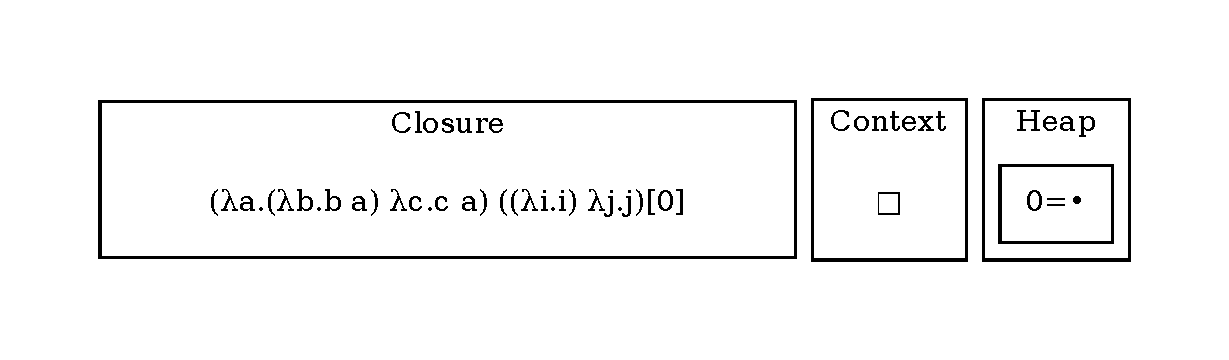
\includegraphics[width=0.99\linewidth/2]{figures/1.pdf}
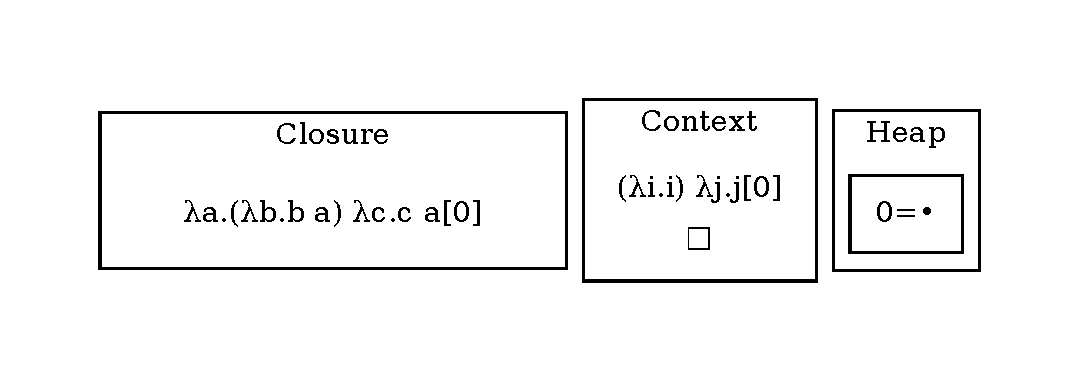
\includegraphics[width=0.99\linewidth/2]{figures/2.pdf}
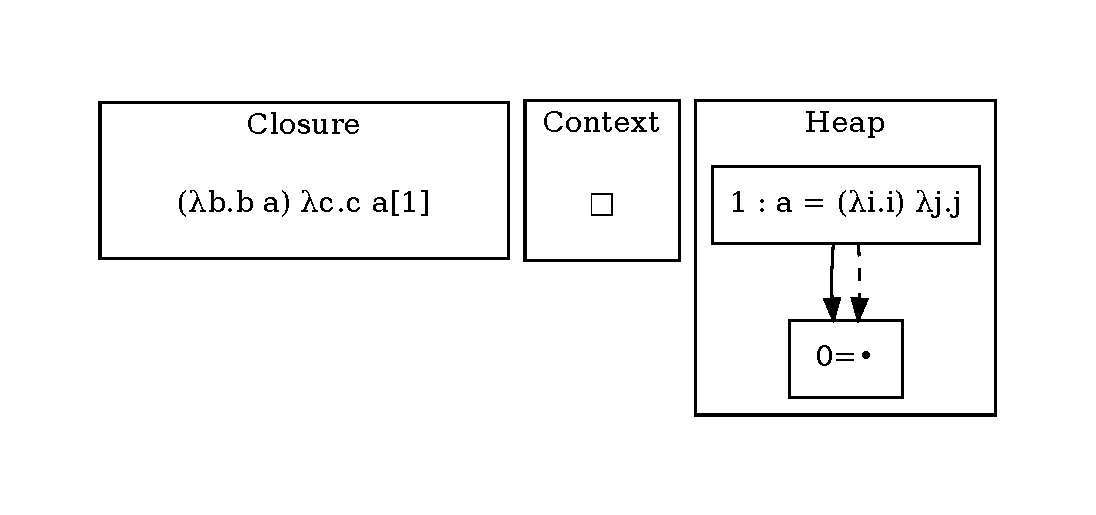
\includegraphics[width=0.99\linewidth/2]{figures/3.pdf}
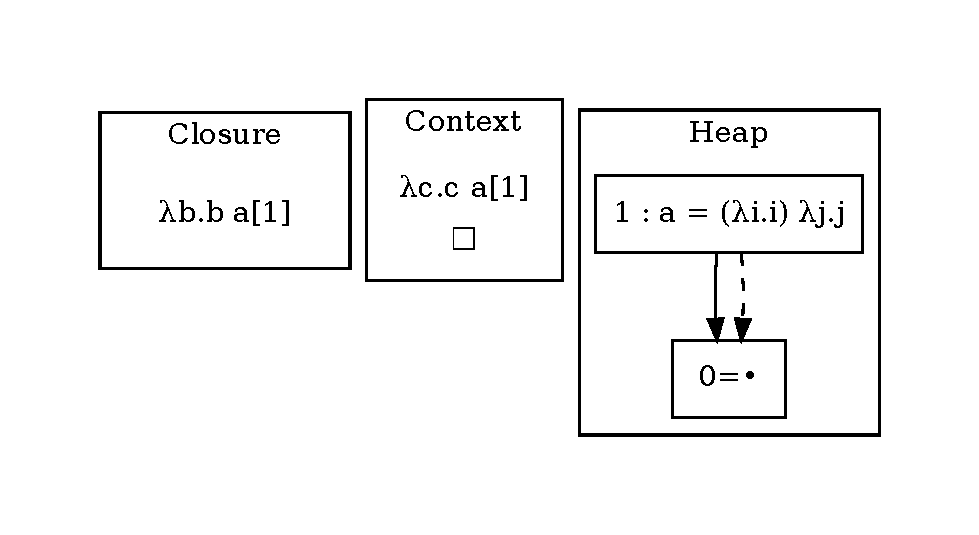
\includegraphics[width=0.99\linewidth/2]{figures/4.pdf}
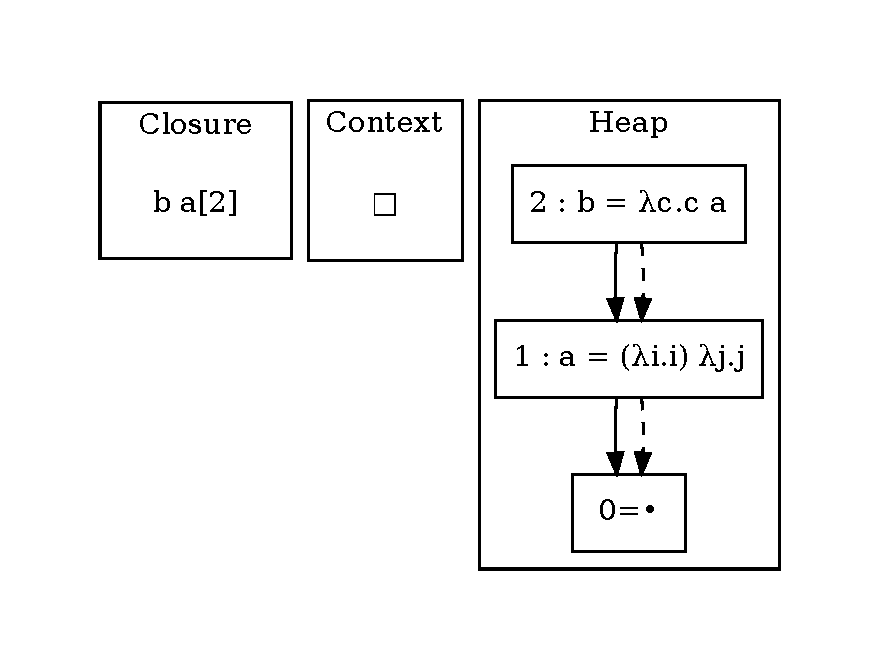
\includegraphics[width=0.99\linewidth/2]{figures/5.pdf}
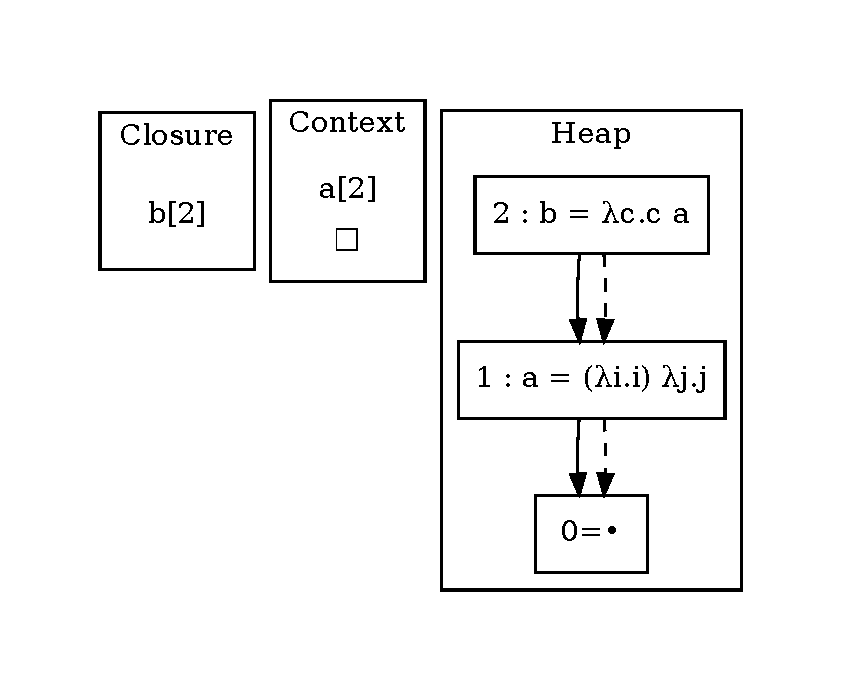
\includegraphics[width=0.99\linewidth/2]{figures/6.pdf}
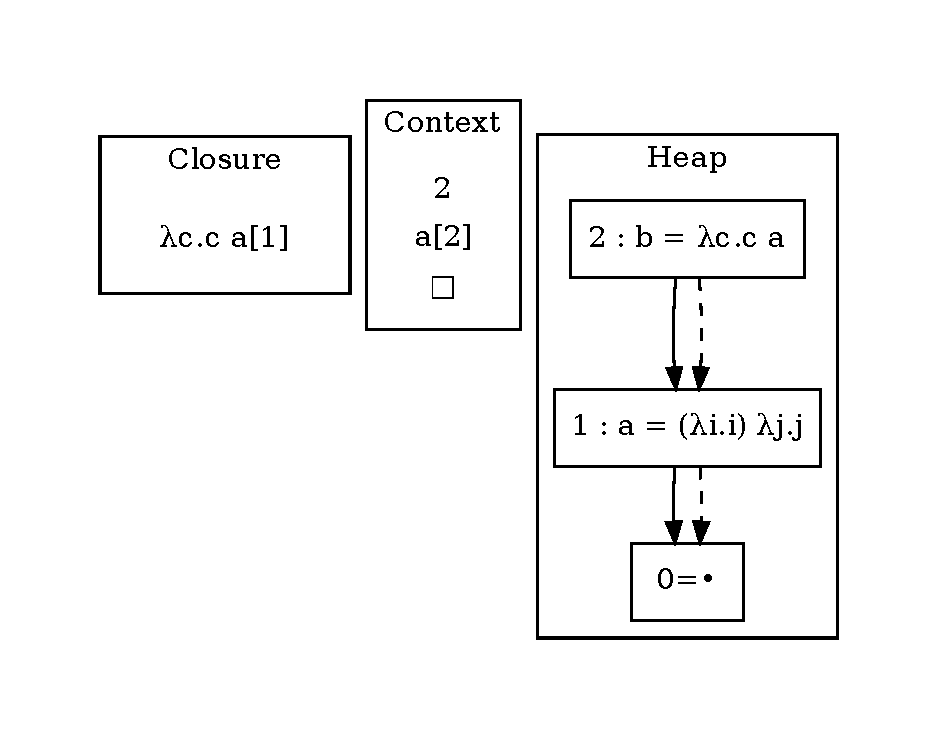
\includegraphics[width=0.99\linewidth/2]{figures/7.pdf}
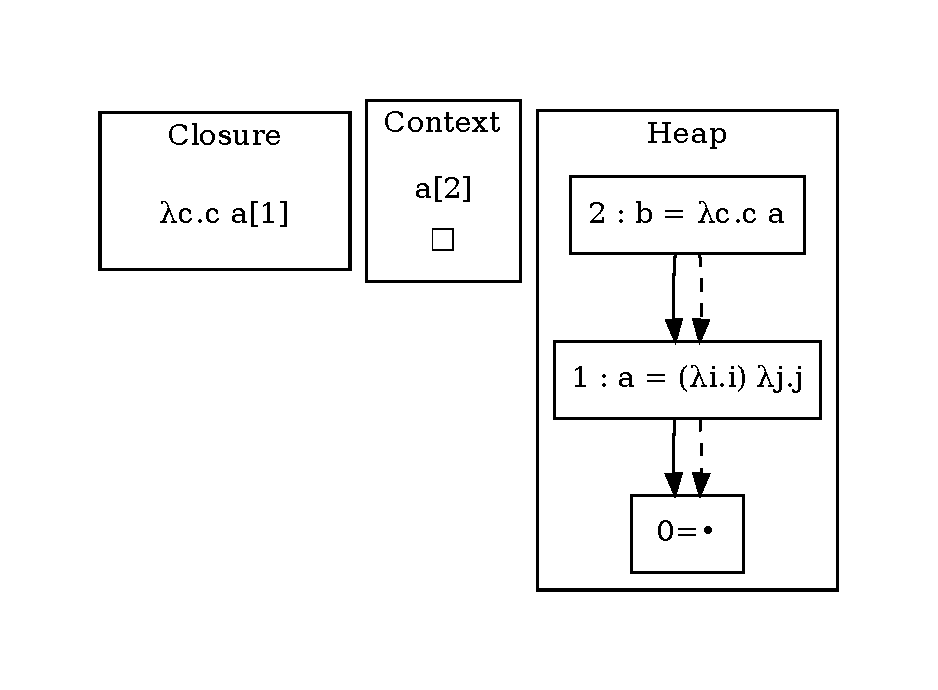
\includegraphics[width=0.99\linewidth/2]{figures/8.pdf}
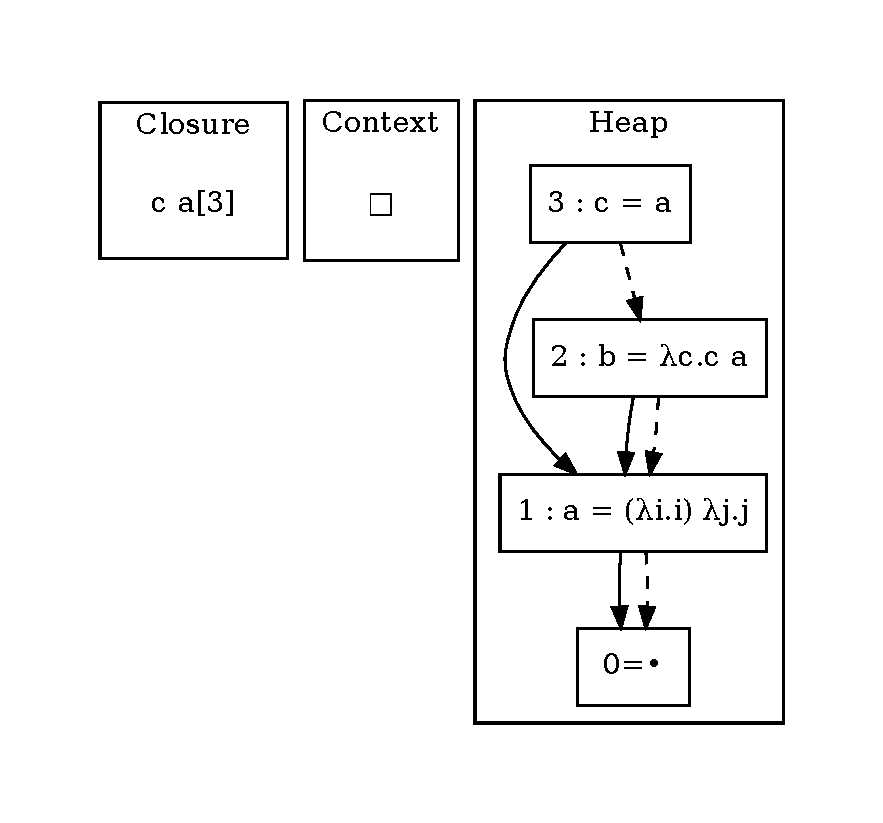
\includegraphics[width=0.99\linewidth/2]{figures/9.pdf}
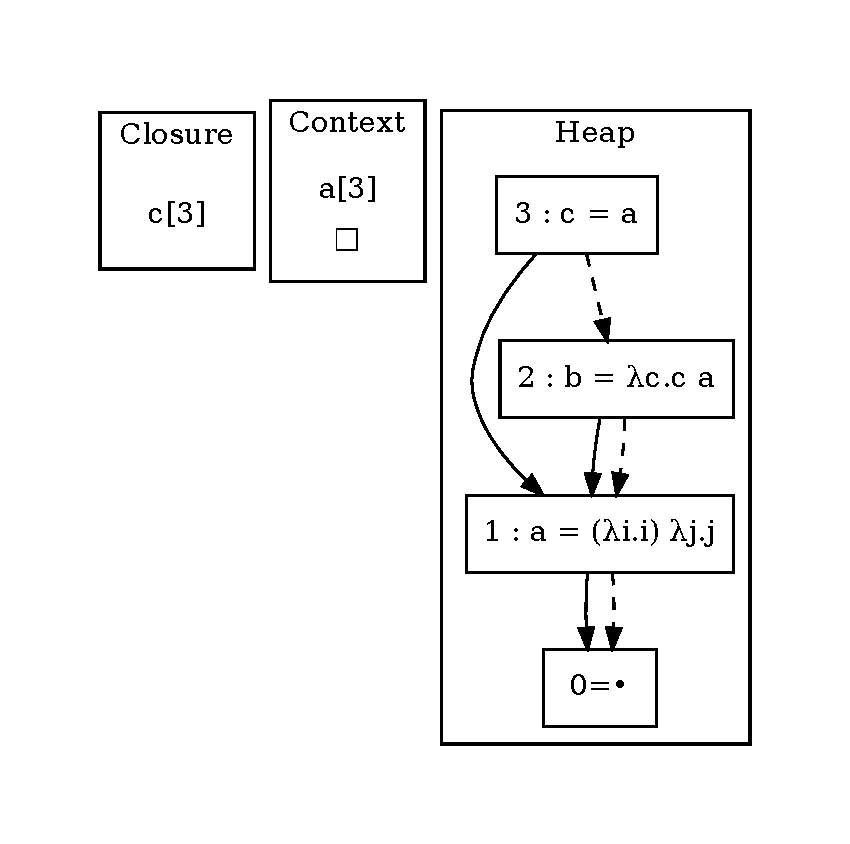
\includegraphics[width=0.99\linewidth/2]{figures/10.pdf}
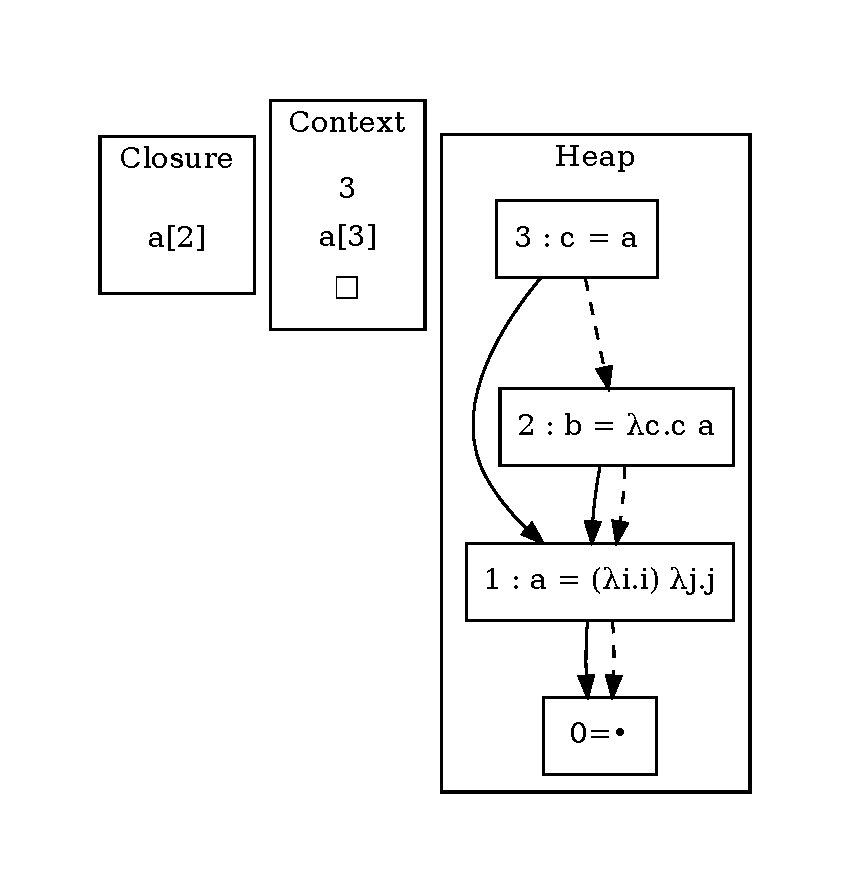
\includegraphics[width=0.99\linewidth/2]{figures/11.pdf}
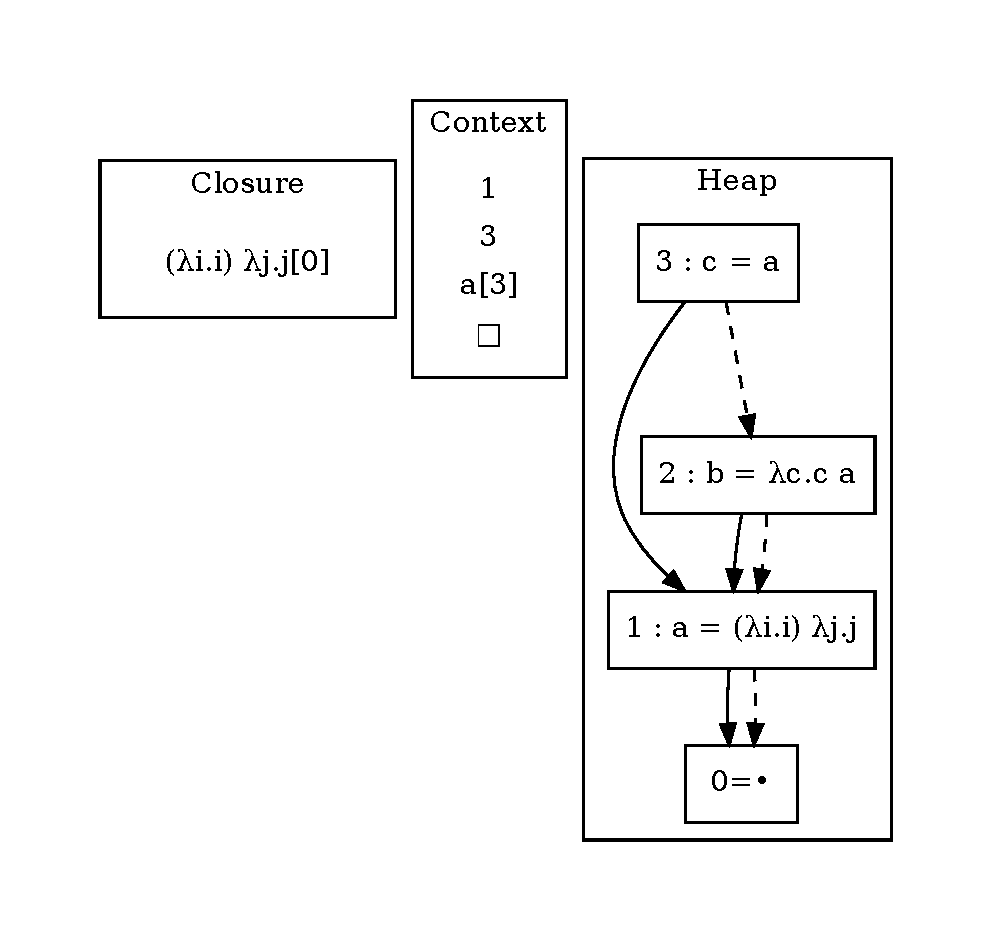
\includegraphics[width=0.99\linewidth/2]{figures/12.pdf}
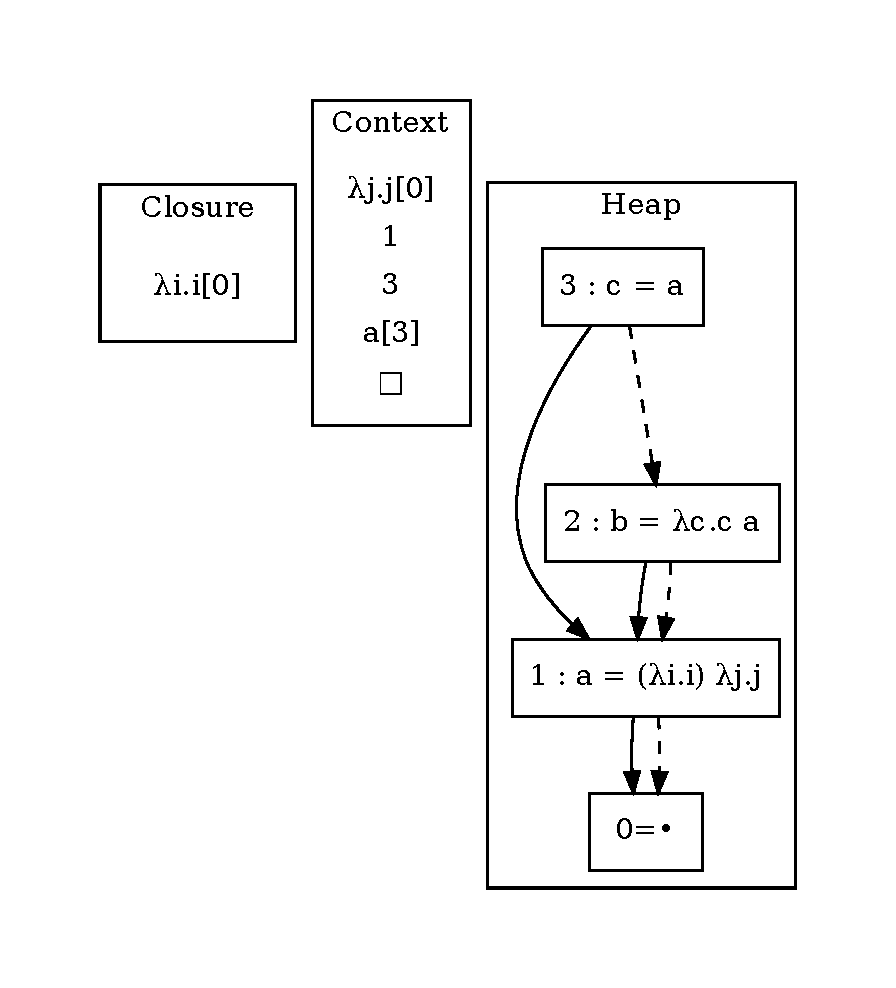
\includegraphics[width=0.99\linewidth/2]{figures/13.pdf}
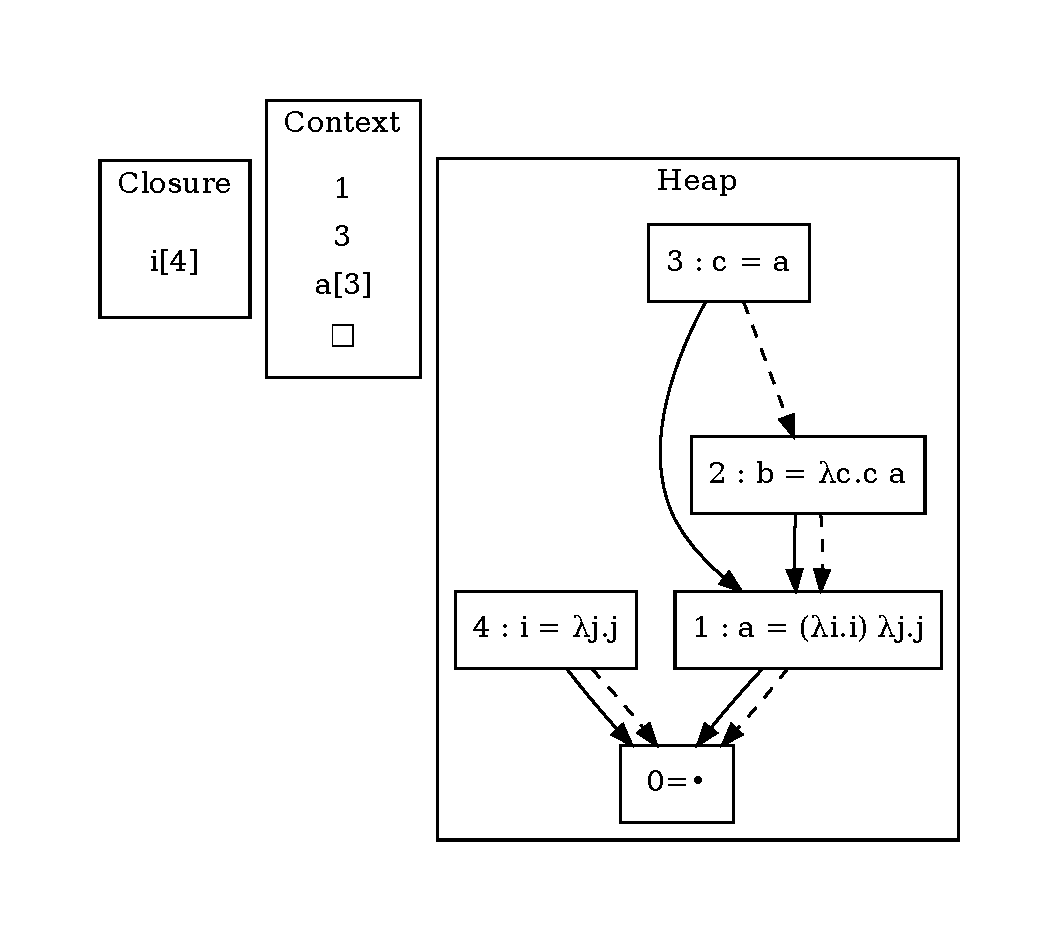
\includegraphics[width=0.99\linewidth/2]{figures/14.pdf}
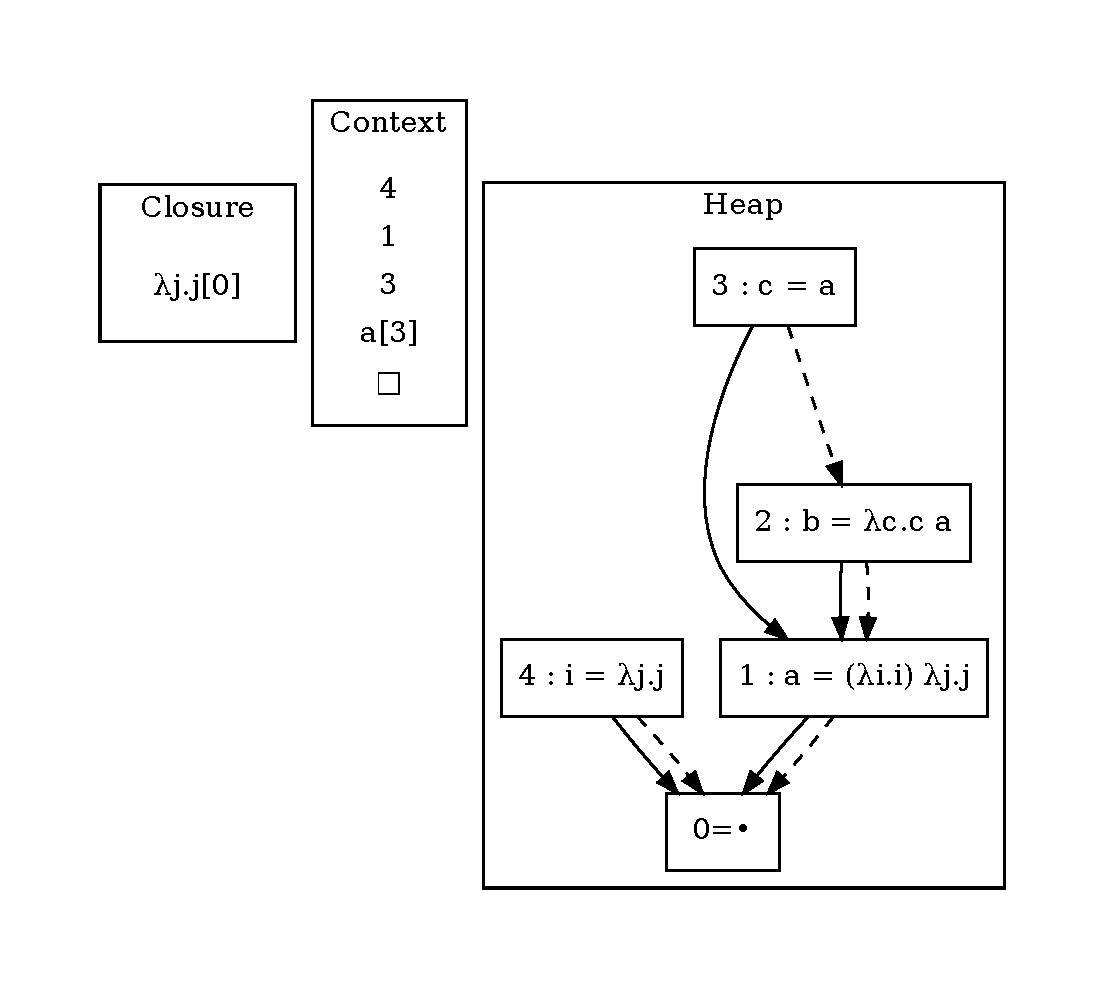
\includegraphics[width=0.99\linewidth/2]{figures/15.pdf}
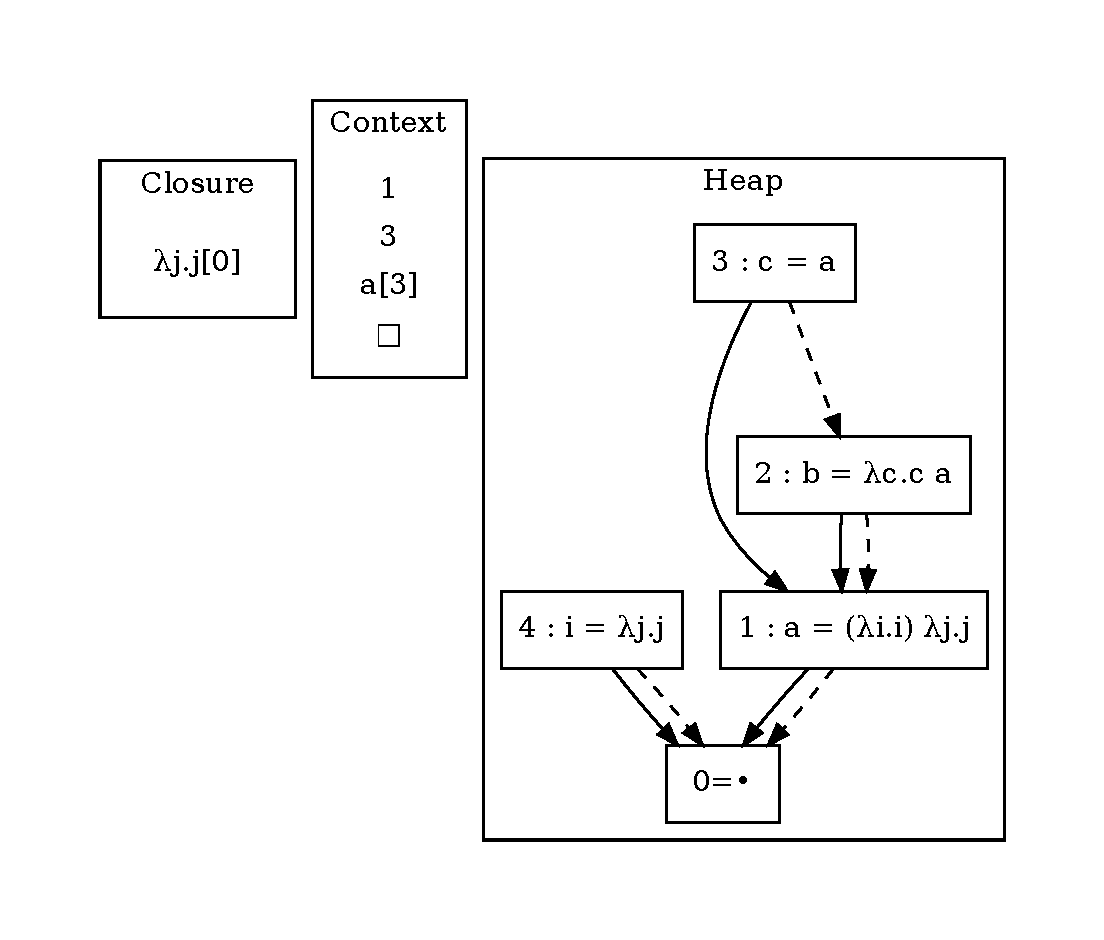
\includegraphics[width=0.99\linewidth/2]{figures/16.pdf}
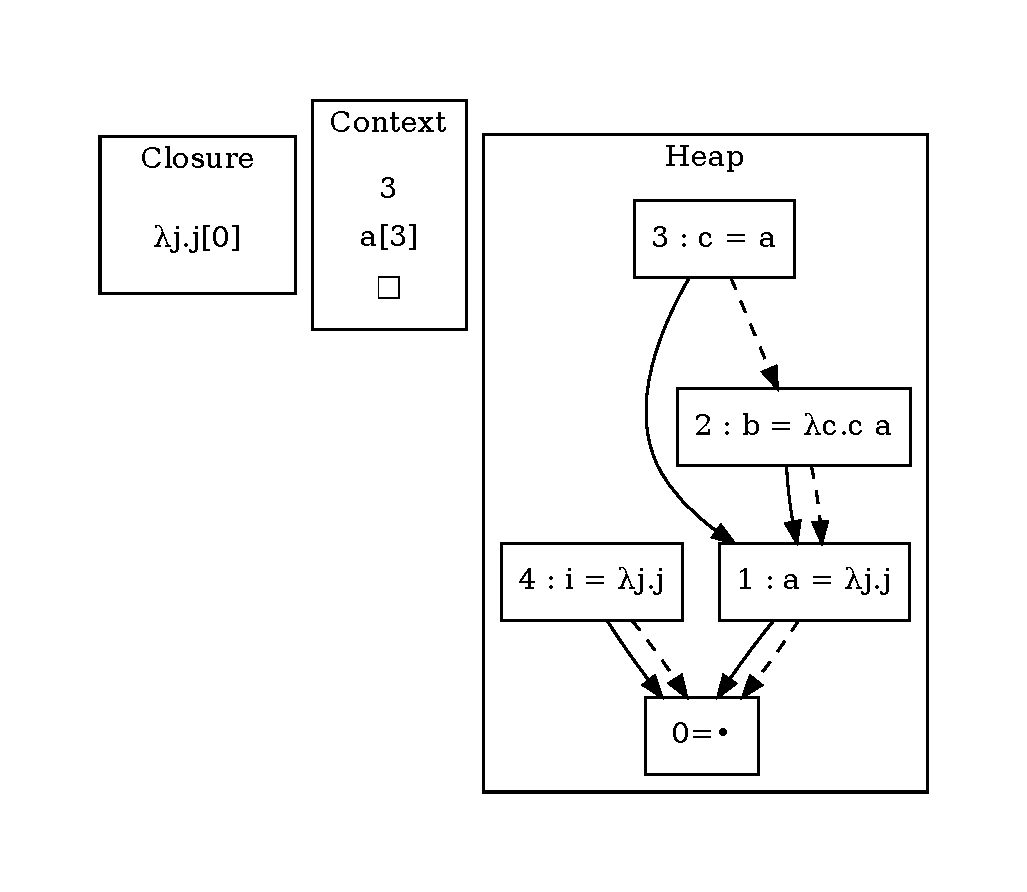
\includegraphics[width=0.99\linewidth/2]{figures/17.pdf}
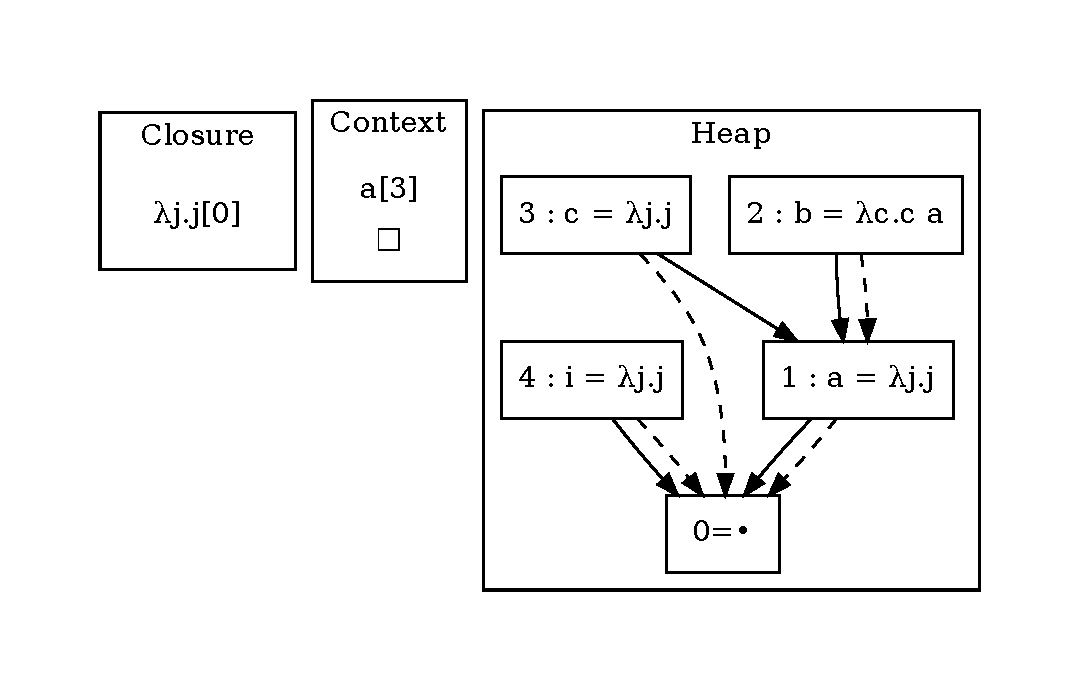
\includegraphics[width=0.99\linewidth/2]{figures/18.pdf}
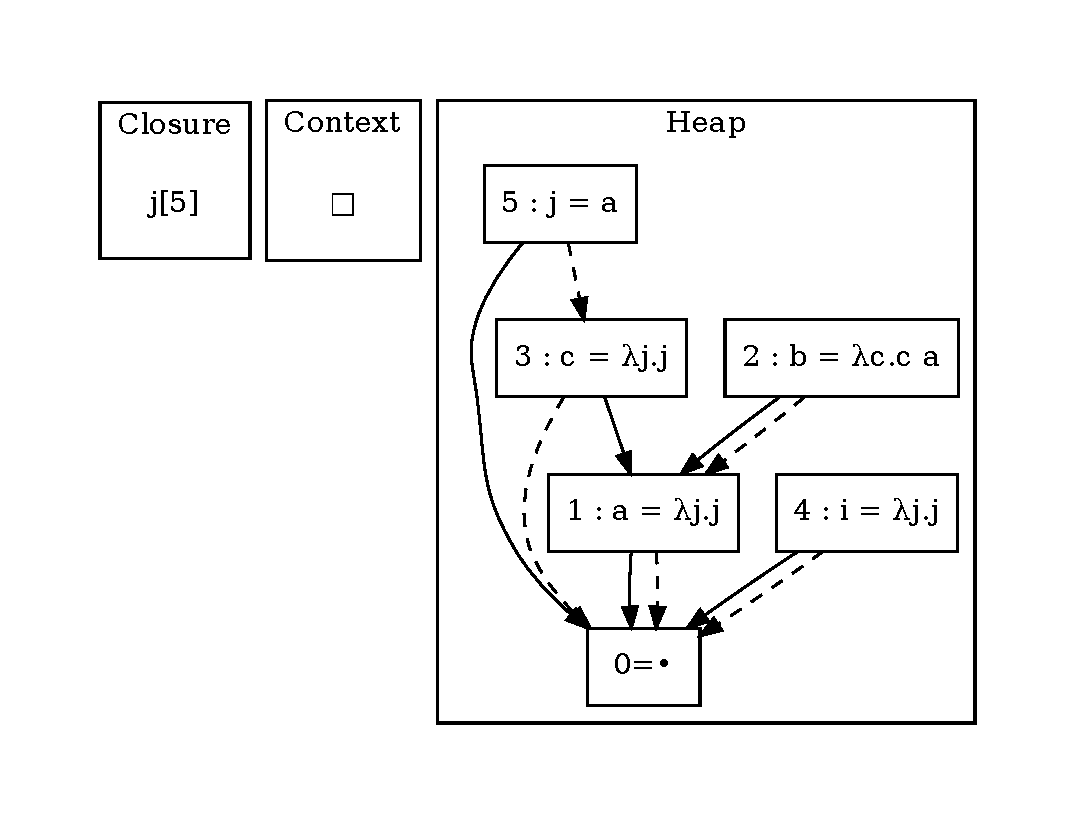
\includegraphics[width=0.99\linewidth/2]{figures/19.pdf}
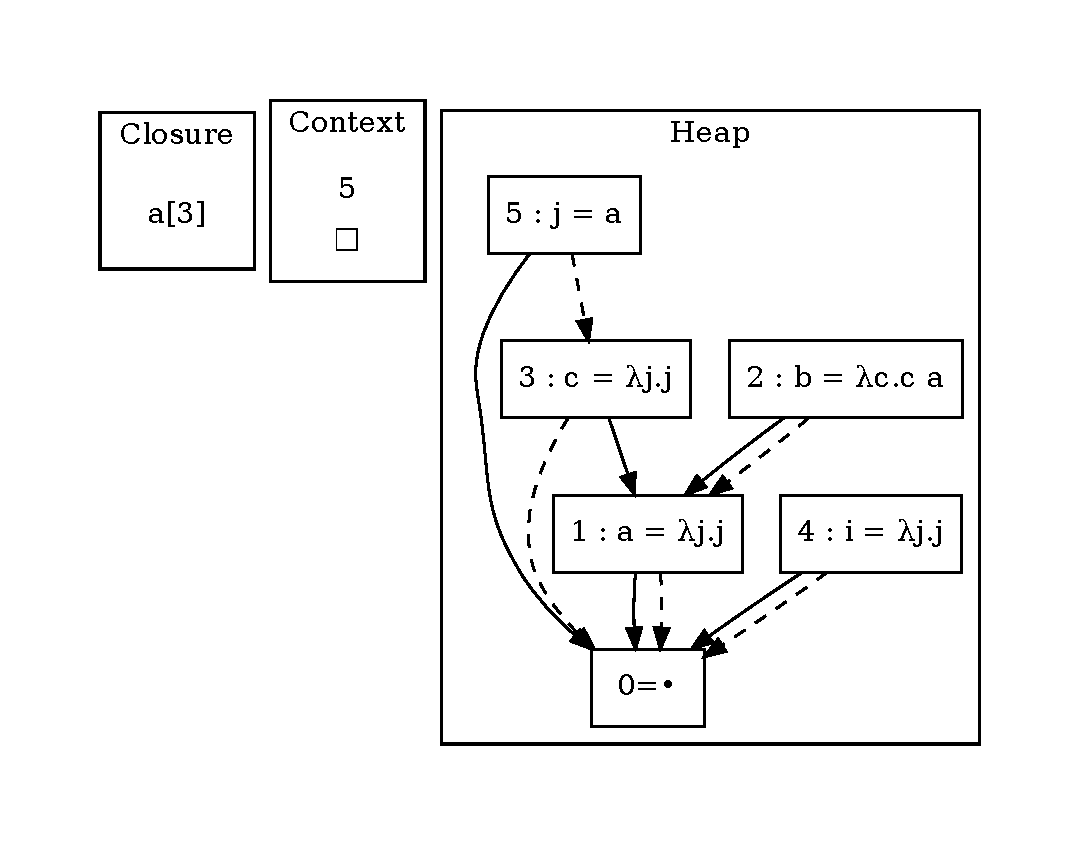
\includegraphics[width=0.99\linewidth/2]{figures/20.pdf}
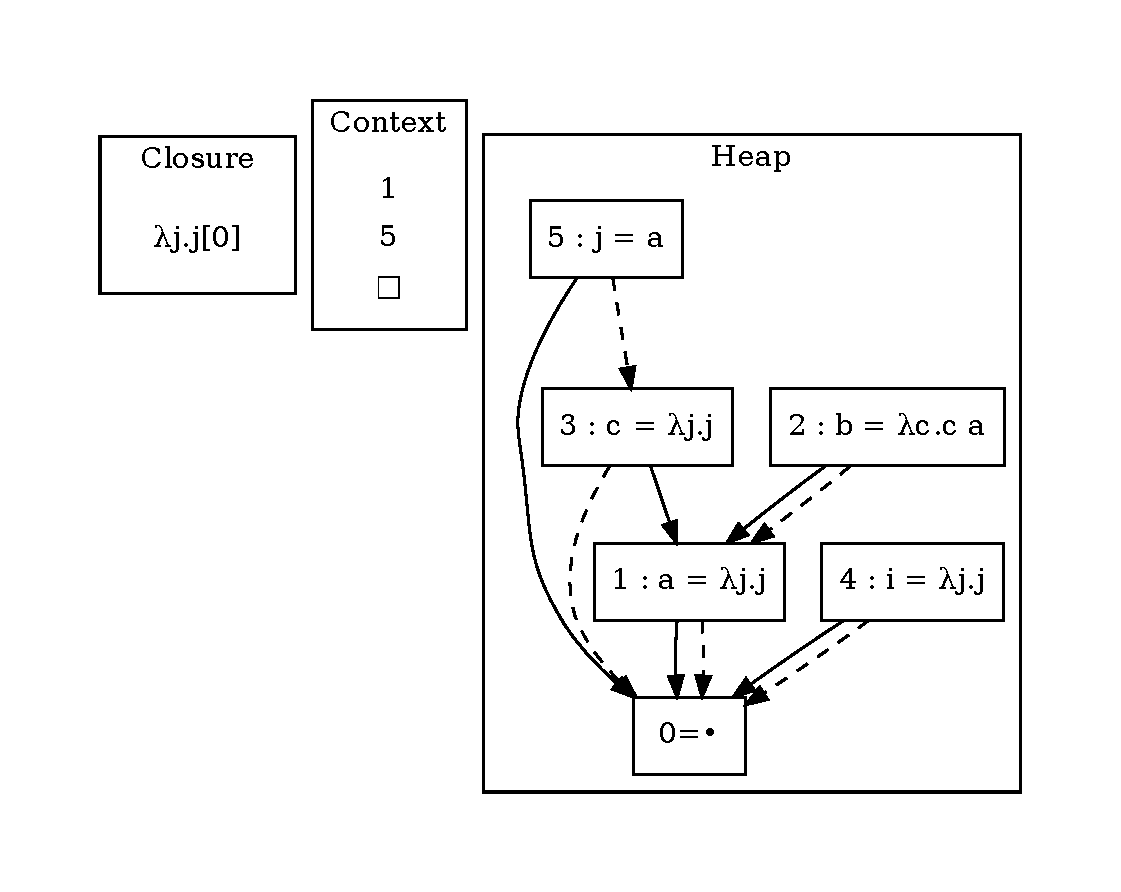
\includegraphics[width=0.99\linewidth/2]{figures/21.pdf}
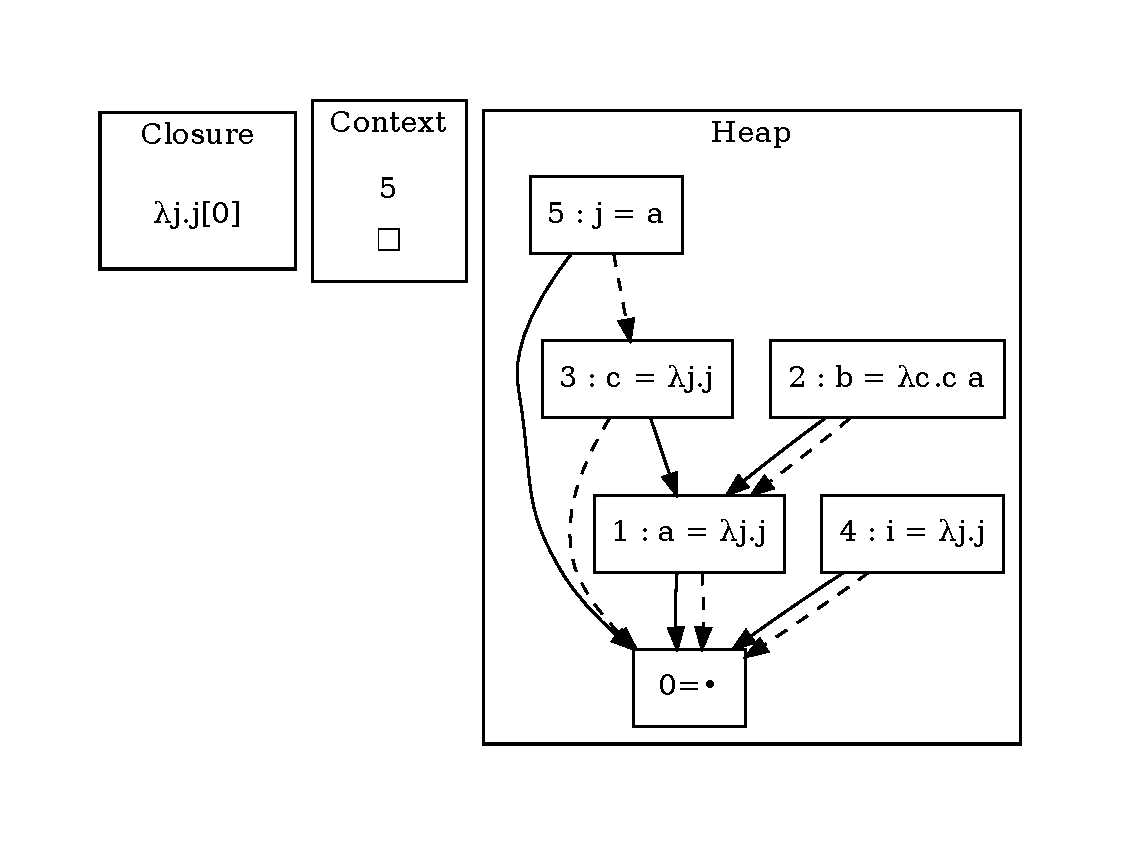
\includegraphics[width=0.99\linewidth/2]{figures/22.pdf}
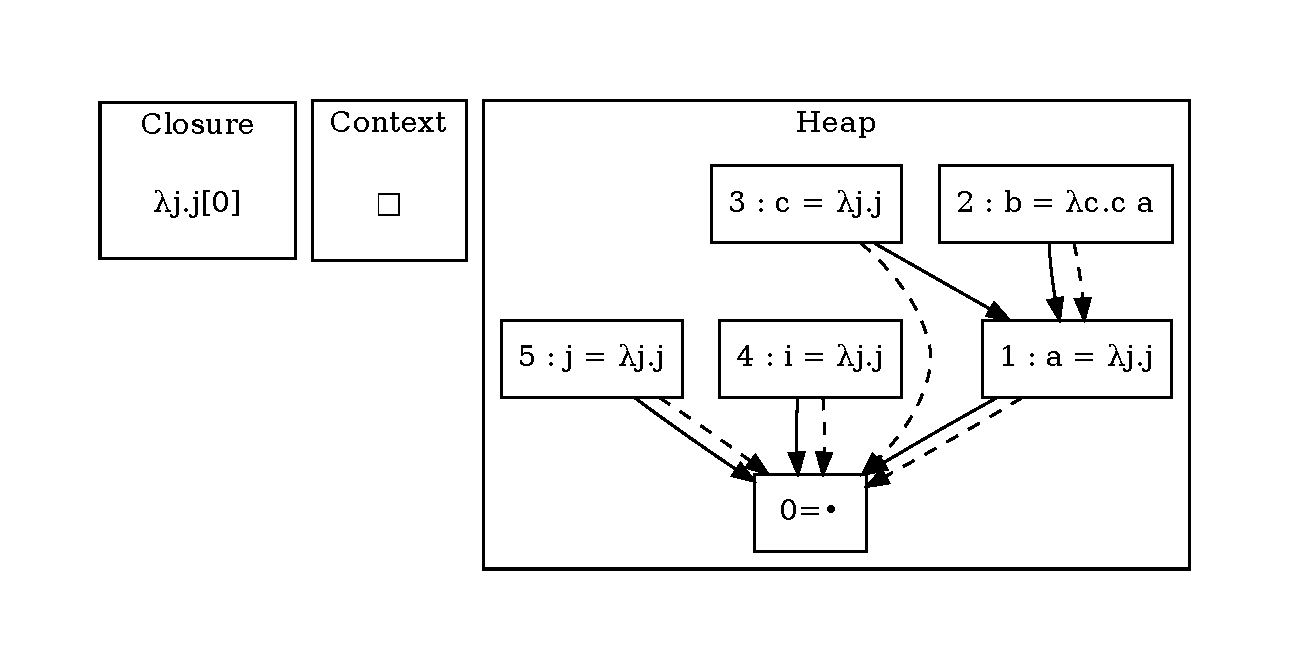
\includegraphics[width=0.99\linewidth/2]{figures/23.pdf}

We can see that through the evaluation, the variable \texttt{a} is dereferenced
twice, in two different scopes. The cactus structure ensures that the value is
correctly shared between the two instances, with the second dereference
correctly dereferencing the evaluated identity function. 

 

\chapter{Coq Implementation Details}\label{chap:coq_appendix}
\chapter{Coq Implementation Details}

Proof irrelevance is an important idea in philosophy of logic. It is the notion
that we don't really need to care how the proof was built, only that it was
sound. In machine checked proofs this notion is particularly relevant: if the
machine checks the proofs of our lemmas, we can be sure that they are valid
proofs.

In contrast, we \emph{must} care about the contents of the definitions and
theorems. Without them, the reader can't be sure what's been proved is what is
being claimed to have been proved. Therefore, we use this section to define and
discuss select Coq definitions and theorem statements in the implementation and
proof of correctness of the verified compiler. We attempt to convey what worked
well, and what posed significant challenges in the hope of informing future work
in this area. The formalization is available at
\url{https://github.com/stelleg/cem\_coq} and as of this dissertation has been
successfully type-checked with Coq version 8.9.  The version used for this
dissertation is tagged with \texttt{dissertation}, which at the time of writing
enables it to be downloaded as a GitHub release tarball. Inevitably, we will use
definitions from both the Coq standard libraries, or generic definitions
implemented throughout the project. In these cases, if the reader has questions,
I encourage them to refer to the source code. In general, this section attempts
to cover the most important definitions and theorems for the 

It's also worth noting that the reader will find many definitions, lemmas,
algorithms, and proofs in the repository that are unused in the final proof.
This is a byproduct of the process of proving. Often, when one starts a proof it
seems like a certain property or lemma will be required, so one proves that
lemma, only to discover later that it was not necessary. Such helper lemmas
sometimes come in useful later, during a different proof. It is for this reason
there are so much unused Coq code in the repository. Hopefully, if the project
is continued, some of them will prove useful.

Another point worth noting is that the Coq code makes heavy use of Unicode
characters and notations. In hindsight, the heavy use of fancy notations was
almost always a mistake, and a refactoring to remove them would likely improve
readability. The one forgivable exception is the occasional infix operator, for
which I make no apologies.

\section{Big-Step \ce Semantics}
Here we define the big step syntax and semantics, which we use as our input
language semantics. This is a formalization of the Figure~\ref{fig:bigstep}.

We start with the lambda calculus with deBruijn indices.

\begin{verbatim}
Inductive tm : Type := 
  | var : nat → tm 
  | lam : tm → tm
  | app : tm → tm → tm.
\end{verbatim}

Next, we define other helper definitions, including closures, environments
(\texttt{env}), cells, heaps, configurations, what doing a lookup into the
shared environment means (\texttt{clu}), and what replacing a closure at a
location in a heap means (\texttt{update}).

\begin{verbatim}
Definition env := nat.

Record closure : Type := close {
  cl_tm : tm;
  cl_en : env
}.

Record cell : Type := cl {
  cell_cl : closure;
  cell_env : env
}.

Definition heap := Map nat cell.

Record configuration : Type := conf {
  conf_h : heap;
  conf_c : closure
}.

Fixpoint clu (v env:nat) (h:heap) : option (nat * cell) := 
  match lookup env h with
  | None => None
  | Some (cl c a) => match v with
    | S n => clu n a h
    | 0 => Some (env, cl c a)
    end
  end.

Fixpoint update (h : heap) (l : env) (v : closure) : heap := match h with 
  | [] => []
  | (u, cl c e)::h => if beq_nat l u 
    then (u, cl v e) :: update h l v 
    else (u, cl c e) :: update h l v
  end.
\end{verbatim}
Finally, we define the actual machine big-step semantics.
\begin{verbatim}
Reserved Notation " c1 '⇓' c2 " (at level 50).
Inductive step : configuration → configuration → Type :=
  | Id : ∀ M x y z Φ Ψ v e, clu y e Φ = Some (x, {M, z}) → 
                    ⟨Φ⟩M ⇓ ⟨Ψ⟩v →
    ⟨Φ⟩close (var y) e ⇓ ⟨update Ψ x v⟩v
  | Abs : ∀ N Φ e, ⟨Φ⟩close (:λN) e ⇓ ⟨Φ⟩close (:λN) e
  | App : ∀ N M B B' Φ Ψ Υ f e ne ae, isfresh (domain Ψ) f → f > 0 →
          ⟨Φ⟩close M e ⇓ ⟨Ψ⟩close (:λB) ne → 
      ⟨Ψ, f ↦ {close N e, ne}⟩close B f ⇓ ⟨Υ⟩close (:λB') ae   →
              ⟨Φ⟩close (M@N) e ⇓ ⟨Υ⟩close (:λB') ae
where " c1 '⇓' c2 " := (step c1 c2).
\end{verbatim}

\section{Small-Step \ce Semantics}

Our small step semantics are a straightforward implementation of the big step
semantics. The language is the same lambda calculus with deBrujn indices, while
we introduce a stack to match marker updates and argument bindings to variables.
This is a formalization of Figure~\ref{fig:cesm}. 

Most of the syntax is shared with the big-step semantics, and is imported
directly from the big-step module. We share the definitions for stacks and
states, followed directly by the small-step semantics.
\begin{verbatim}
Definition stack := list (closure + nat).

Inductive state : Type := st {
  st_hp : heap; 
  st_st : stack;
  st_cl : closure
}.

Reserved Notation " c1 '→_s' c2 " (at level 50).
Inductive step : transition state :=
  | Upd : ∀ Φ b e l s, 
  st Φ (inr l::s) (close (lam b) e) →_s 
  st (update Φ l (close (lam b) e)) s (close (lam b) e)
  | Var : ∀ Φ s v l c e e', clu v e Φ = Some (l,cl c e') → 
  st Φ s (close (var v) e) →_s st Φ (inr l::s) c
  | Abs : ∀ Φ b e f c s, isfresh (domain Φ) f → f > 0 → 
  st Φ (inl c::s) (close (lam b) e) →_s st ((f, cl c e):: Φ) s (close b f)
  | App : ∀ Φ e s n m, 
  st Φ s (close (app m n) e) →_s st Φ (inl (close n e)::s) (close m e)
where " c1 '→_s' c2 " := (step c1 c2).
\end{verbatim}

\subsection{Relation to Big-Step}

We prove that the small step semantics implement the big step semantics with the
following lemma. The description of the proof can be found in
Section~\ref{sec:cem_cesm}. 

\begin{verbatim}
Notation " c1 '→_s*' c2 " := 
  (refl_trans_clos cesm.step c1 c2) (at level 30). 

Lemma cem_cesm : ∀ Φ Ψ c v, 
  conf Φ c ⇓ conf Ψ v → ∀ s, 
  st Φ s c →_s* st Ψ s v. 
\end{verbatim}

\section{Instruction Machine} 

Finally, we change representations and describe the assembly language of the
abstract instruction machine; the target of the verified compiler. This is the
formalization of language defined in Figure~\ref{fig:im_syntax}. Note the use of
coercions to help ease the use of type-safe read and write operands, and an
infix operator to duplicate common syntax for real world assembly languages when
indexing an offset. Note that for our purposes, we only ever need a constant
offset, but one could easily extend the language to allow for offsets to be
defined by a read operand.  

\begin{verbatim}
Definition Word := nat.
Definition Ptr := nat.

Inductive Reg := 
  | IP
  | EP
  | R1
  | R2.

Inductive WO := 
  | WR : Reg → WO
  | WM : Reg → nat → WO.

Coercion WR : Reg >-> WO.
Infix "%" := WM (at level 30).

Inductive RO := 
  | RW : WO → RO
  | RC : nat → RO.

Coercion RW : WO >-> RO.
Coercion RC : nat >-> RO.

Inductive Instr : Type :=
  | push : RO → Instr
  | pop : WO → Instr
  | new : nat → WO → Instr 
  | mov : RO → WO → Instr.

Inductive BasicBlock : Type :=
  | instr : Instr → BasicBlock → BasicBlock
  | jump : option (RO*Ptr) → RO → BasicBlock.

Definition Program := list BasicBlock.
\end{verbatim}

Finally, note that we use a list of basic blocks as our program. This list is
indexed by integers in the machine semantics, so translating this to a Harvard 
architecture machine semantics should be relatively straightforward. 

Now that we have the language for our abstract instruction machine target, we
can look at the formal semantics for it. Without loss of generality, we choose a
step relation on instructions, wrapped by a step instruction on full basic
blocks. This eases reasoning about the relation to the small step \ce
relation. This is a formalization of the semantics described in
Figure~\ref{fig:im_semantics}. 

We start with a our register file and machine state, along with a
straightforward semantics for reading and writing from operands given a 
machine state. We omit some uninteresting helper functions. 

\begin{verbatim}
Inductive RegisterFile := mkrf {
  ip : Ptr;
  ep : Ptr;
  r1 : Ptr; 
  r2 : Ptr
}. 

Inductive State := st {
  st_rf : RegisterFile;
  st_p : Program;
  st_s : Stack;
  st_h  : Heap
}.

Open Scope nat_scope. 
Inductive read : RO → State → Ptr → Type :=
  | read_reg : ∀ r s, read (RW (WR r)) s (rff (st_rf s) r)
  | read_mem : ∀ r o rf p s h v, 
    lookup (o+rff rf r) h = Some v →
    read (RW (WM r o)) (st rf p s h) v
  | read_const : ∀ c s, read (RC c) s c.

Inductive write : WO → Word → State → State → Type :=
  | write_reg : ∀ r rf p s h w, 
    write (WR r) w (st rf p s h) (st (upd r w rf) p s h)
  | write_mem : ∀ r o rf p s h w, 
    write (WM r o) w (st rf p s h) 
                     (st rf p s (replace beq_nat (o+rff rf r) w h)).
\end{verbatim}

Given our machine definitions and read and write semantics, we can move directly
to defining the step relation for instructions. The \texttt{step\_bb} relation
defines the execution of a full basic block by induction on the instructions
contained in that basic blocks. The \texttt{step} relation then wraps that
relation and defines how the state changes given execution of the basic block
pointed to by the instruction pointer. Note that we don't define an explicit
halting relation. Instead, the machine will be stuck when the current code to be
executed is a value and the stack is empty, which is where the small step
\ce semantics also get stuck. In contrast, the native code implementation has a
check to ensure the stack is non-empty. A full compiler with a sufficiently
sophisticated type system could likely do away with this check, only terminating
with the \texttt{main} function returning a value of type \texttt{World}. 

\begin{verbatim}
Inductive step_bb : BasicBlock → State → State → Type := 
  | step_push : ∀ rf p s h ro is v sn,
  read ro (st rf p s h) v → 
  step_bb is (st rf p (v::s) h) sn → 
  step_bb (instr (push ro) is) (st rf p s h) sn
  | step_pop : ∀ rf p s h wo is w s' sn,
  write wo w (st rf p s h) s' → 
  step_bb is s' sn →
  step_bb (instr (pop wo) is) (st rf p (w::s) h) sn
  | step_new : ∀ rf p s h wo is w s' n sn,
  (∀ i, i < n → not (In (i+w) (domain h))) →
  w > 0 →
  write wo w (st rf p s (zeroes n w ++ h)) s' →
  step_bb is s' sn → 
  step_bb (instr (new n wo) is) (st rf p s h) sn 
  | step_mov : ∀ s is ro wo s' v sn, 
  read ro s v → write wo v s s' → 
  step_bb is s' sn → 
  step_bb (instr (mov ro wo) is) s sn
  | step_jump0 : ∀ ro k j s s', 
  read ro s 0 →
  write (WR IP) k s s' → 
  step_bb (jump (Some (ro, k)) j) s s'
  | step_jumpS : ∀ ro k j s s' l k', 
  l > 0 →
  read ro s l →
  read j s k → 
  write (WR IP) k s s' → 
  step_bb (jump (Some (ro, k')) j) s s'
  | step_jump : ∀ ro s s' l, 
  read ro s l →
  write (WR IP) l s s' → 
  step_bb (jump None ro) s s'
.

Inductive step : transition State :=
  | enter : ∀ rf p s h k bb sn,
    read IP (st rf p s h) k → 
    nth_error p k = Some bb → 
    step_bb bb (st rf p s h) sn →
    step (st rf p s h) sn.
\end{verbatim}

With our step function defined, we can start thinking about how we want to
implement our compiler, and how to relate the instruction machine to the small
step semantics of our input language.  

\subsection{Relation to Small-Step Semantics}

We now have everything we need, except for the compiler definition, which we
will address in the next section. We start by assuming a \texttt{new} function,
which is effectively a \texttt{malloc} that given a heap, returns a non-null
free contiguous region of memory. Of course, in reality \texttt{malloc} is a
partial function, but we aren't modelling running out of memory in this work. 

\begin{verbatim}
Variable new : ∀ (n:nat) (h : im.Heap), sigT (λ w:nat, 
  prod (∀ i, lt i n → (i+w) ∉ domain h)
       (w > 0)).

Definition prog_eq (p : Ptr) (pr : Program) (t : tm) := 
  let subpr := assemble t p in subpr = firstn (length subpr) (skipn p pr).
\end{verbatim}

Next, we discuss heap relations between the instruction machine and the \ce \\
machine semantics. Unfortunately, this gets incredibly involved. Despite much
effort, I was unable to find a more elegant relation between the two.

\begin{verbatim}
Inductive heap_rel : cesm.heap → im.Heap → Type := 
  | heap_nil : heap_rel [] [] 
  | heap_cons : ∀ l l' ne ch ih ip ep ine e t, 
    l ∉ domain ch → l' ∉ domain ih → 
    S l' ∉ domain ih → S (S l') ∉ domain ih →
    l > 0 → l' > 0 → 
    heap_rel ch ih → 
    heap_rel 
      ((l, cl (close t e) ne)::ch) 
      ((l', ip)::(S l', ep)::(S (S l'), ine)::ih).

Fixpoint in_heap_rel (ch : cesm.heap) (ih : im.Heap)
                     (r : heap_rel ch ih)
                     (l e ne : nat) (t : db.tm) 
                     (il ip ep nep : Ptr) : Type := match r with
  | heap_nil => False
  | heap_cons l' il' ne' cht iht ip' ep' nep' e' t' _ _ _ _ _ _ rt => 
    if andb (beq_nat l l') (beq_nat il il') then
    (ne' = ne) *  (ip' = ip) * (ep' = ep) * 
    (nep' = nep) * (e' = e) * (t' = t)
    else 
      if andb (negb (beq_nat l l')) (negb (beq_nat il il'))
        then in_heap_rel cht iht rt l e ne t il ip ep nep
        else False
  end.

Inductive env_eq (ch : cesm.heap) (ih : im.Heap) (r : heap_rel ch ih)
  : nat → Ptr → Type :=
  | e0 : env_eq ch ih r 0 0 
  | eS : ∀ l e ne t il ip ep nep, 
    in_heap_rel ch ih r l e ne t il ip ep nep →
    env_eq ch ih r l il.

Inductive heap_eq (ch : cesm.heap) (ih : im.Heap) 
                  (r : heap_rel ch ih) (p : Program) : Type := 
  | mkheap_eq : 
    (∀ l e ne t il ip ep nep, 
      in_heap_rel ch ih r l e ne t il ip ep nep →
      (prog_eq ip p t) * 
      (env_eq ch ih r e ep) * 
      (env_eq ch ih r ne nep)) → 
    heap_eq ch ih r p.

\end{verbatim}

In words, the \texttt{heap\_rel} defines a heap relation that simply relates an
entry in the \ce heap to the three machine words in the instruction machine
heap. \texttt{in\_heap\_rel} is a decidable relation that determines whether or
not a given heap location and cell at that location and their corresponding
machine analogues are related by a heap relation object. We say environments are
equal if they are either both the empty environment or the first element of the
environments are in the heap relation, and the tails are equal. Two heaps are
equivalent if for every cell, the term portions are equivalent and the
environment and environment continuations are equivalent. The inductive relation
on the environments is crucial for inductive reasoning on deBruijn indices.

Given our heap and environment relations, we can move to notions of closure,
stack, and complete state equivalences.

\begin{verbatim}
Inductive clos_eq (ch : cem.heap) (ih : im.Heap) 
                  (r : heap_rel ch ih) (p : Program):
                  closure → Ptr → Ptr → Type :=
  | c_eq : ∀ t e ip ep, 
           prog_eq ip p t → 
           env_eq ch ih r e ep →
           clos_eq ch ih r p (cem.close t e) ip ep. 

Inductive stack_eq (ch : cem.heap) (ih : im.Heap) 
                   (r : heap_rel ch ih) (p : Program) : 
  cesm.stack → im.Stack → Type := 
  | stack_nil : stack_eq ch ih r p nil nil
  | stack_upd : ∀ l e ne t il ip ie ine cs is, 
                in_heap_rel ch ih r l e ne t il ip ie ine →
                stack_eq ch ih r p cs is →
                stack_eq ch ih r p (inr l::cs) (0::il::is)
  | stack_arg : ∀ ip ep cs is c, 
                 ip > 0 →
                 clos_eq ch ih r p c ip ep →
                 stack_eq ch ih r p cs is → 
                 stack_eq ch ih r p (inl c::cs) (ip::ep::is).

Inductive state_rel (cs : cesm.state) (is : im.State) : Type := 
  | str : ∀ r, 
  heap_eq (st_hp cs) (st_h is) r (st_p is) →
  clos_eq (st_hp cs) (st_h is) r (st_p is) (st_cl cs) 
          (rff (st_rf is) IP) (rff (st_rf is) EP) →
  stack_eq (st_hp cs) (st_h is) r (st_p is) (st_st cs) (st_s is) →
  state_rel cs is.
\end{verbatim}
For the stack relation, we have either the empty stacks or two stacks with
either both update markers or both argument closures on top, and equivalent
stacks below that. For update markers, we have that the two marker locations
exist in the heap relation. For argument closures, we have that the closures are
equivalent. 

The closure and state relations are straightforward, the closure relation
requires that the term and subprogram are equal, and that the environments are
equivalent. The state relation requires equivalent closure and registerfile
entries (IP and EP), equivalent heaps, and equivalent stacks.

Finally, we can pose our lemma that the instruction machine implements the
small-step semantics.

\begin{verbatim}
Lemma cesm_im : ∀ v s s', state_rel s s' → 
  cesm.step s v → 
  sigT (λ v', prod (refl_trans_clos im.step s' v') (state_rel v v')).
\end{verbatim}
This states that if we have related small step and instruction machine states,
and we take a small step, then the instruction machine will take a step to a
state that is related to the new state of the small-step machine.  While we
don't discuss the proof in detail, it's worth mentioning that even with many
supporting definitions and lemmas, it took on the order of 2000 Ltac statements
to prove. Note that is a single step, but the reflexive transitive closure
version follows trivially. 

\section{Compiler and Correctness}

We've seen the \texttt{assemble} function referred to relate the lambda terms to
the machine instructions in the previous section. This sections defines that
function, which is the entire compiler implementation.

\begin{verbatim}
Infix ";" := instr (at level 30, right associativity).

Fixpoint var_inst (i : nat) : BasicBlock := match i with
  | 0 => push EP ;
         push (RC 0) ;
         mov (EP%0) R1 ;
         mov (EP%1) EP ;
         jump None R1
  | S i => mov (EP%2) EP ; 
           var_inst i
  end.


(* Assembles deBruijn indices to instructions *)
Fixpoint assemble (t : tm) (k : nat) : Program := match t with  
  | var v => [var_inst v]
  | app m n => let ms := assemble m (1+k) in
               let nk := 1+k+length ms in
                push EP ;
                push (RC nk) ;
                jump None (RC (1+k)) :: 
                ms ++ 
                assemble n nk
  | lam b => pop R1 ;
             jump (Some (RW (WR R1), (1+k))) (RC (2+k)) ::
             (*Update*)
             pop R1 ;  
             mov (RC k) (R1%0) ;
             mov EP (R1%1) ;
             jump None (RC k) ::
             (*Take*)
             new 3 R2 ;
             mov R1 (R2%0);
             pop (R2%1) ;
             mov EP (R2%2) ;
             mov R2 EP ;
             jump None (3+k) :: 
             assemble b (3+k)
  end. 
\end{verbatim}
We can see that the compiler is very simple, only requiring ~35 lines of code.
It is this simplicity that enables the formal reasoning achieved in the previous
section. 

Finally, we can define our top level correctness theorem.

\begin{verbatim}
Definition compile t := assemble t 0.

Theorem compile_correct (t : db.tm) v : cem.step (cem.I t) v → 
  sigT (λ v', refl_trans_clos im.step (im.I (compile t)) v' *
              state_rel (cesm.st (cem.conf_h v) nil (cem.conf_c v)) v').
\end{verbatim}
This theorem states that if a term steps in the big step semantics to a value,
then the instruction machine will step in zero or more steps to a related state.
Knowledge of the \texttt{state\_rel} relation is crucial here: it would be
trivial to define a meaningless relation, e.g. the relation defined by
\texttt{λ c i, True}, and prove the relation trivially. Because we know that
the relation requires equivalence of term and subprogram pointed to by IP, we
know that the theorem is what we want.

TODO: Add definitions and theorems for relation to curiens calculus of closures.
 

\bibliographystyle{amsplain}
\bibliography{annotated}

\end{document}
